\documentclass[a4paper, onecolumn, 12pt]{IEEEtran}
%\documentclass[draftcls, onecolumn, a4paper, twoside]{IEEEtran}


% These values get used many times, so it is easier to define then once here.
% Module code
\def\modulecode{ELI 220}
% Module name
\def\modulename{Linear Systems and Signals}
% Assessment title
\def\assessment{Practical 1}
\def\assessmenttitle{The Fourier Series}
% Group number
\def\groupnumber{43}

% Student details: (Leave blank the last student(s) if your group has fewer people. The contributions MUST add up to 100%. Additional rows in the table on the title page can be commented out in titlepage.tex.)
% Details of the first student
\def\firststudentname{Emma Muller}
\def\firststudentnumber{24875882}
\def\firststudentcontribution{33.33}
% Details of the second student
\def\secondstudentname{Jan-Hendrik Brink}
\def\secondstudentnumber{23694956}
\def\secondstudentcontribution{33.33}
% Details of the third student
\def\thirdstudentname{Sean van Wyk}
\def\thirdstudentnumber{24606872}
\def\thirdstudentcontribution{33.33}

% Allows multi-line equations to be split over a number of pages.
\interdisplaylinepenalty=2500 


\usepackage{amsmath}
\usepackage{amssymb}
\usepackage{cite}
\usepackage{graphicx}
\usepackage{lastpage}
\usepackage{listings}
\usepackage{minted}
\usepackage{multirow}
\usepackage{paralist}
\usepackage{placeins}  % For \FloatBarrier
%\usepackage{rotfloat}
\usepackage{rotating}
\usepackage[tight,small]{subfigure}  % normalsize small footnotesize
\usepackage{tabularx}
\usepackage{tabulary}


% I prefer this to the default font.
\usepackage{newtxmath}
% \usepackage{newtxtext}
\renewcommand{\rmdefault}{ntxtlf} 
%https://tex.stackexchange.com/questions/347566/math-digits-are-rendered-in-cm-when-using-libertine-and-newtxmath-with-xelatex-i


% Set the page format up.
\usepackage{geometry}
\geometry{includefoot}
\geometry{paper=a4paper}
\geometry{left=25mm}
\geometry{right=25mm}
\geometry{top=25mm}
\geometry{bottom=20mm}
\geometry{headsep=10mm}
\geometry{footskip=10mm}
%\geometry{columnsep=4mm}




\usepackage[pdftex]{hyperref}
%\hypersetup{pdfborder={0 0 0.2}}
\usepackage{xcolor}
\definecolor{darkred}{rgb}{0.8,0,0}
\definecolor{darkgreen}{rgb}{0,0.45,0}
\definecolor{darkblue}{rgb}{0,0,0.3}
\hypersetup{colorlinks=True, citecolor=black, filecolor=black, linkcolor=black, urlcolor=black}

% Set the PDF properties of the document.
\hypersetup{%
  pdftitle={\modulecode-- \assessment: \assessmenttitle},
  pdfauthor={Group \groupnumber}}


\usepackage[acronym,nonumberlist,nopostdot,style=super]{glossaries}  % This must be after hyperref.

% Load the abbreviations.
% \loadglsentries{abbreviations}
% \makeglossaries

% % Format the abbreviations list.
% \renewenvironment{theglossary}%
% {%\vspace{-1em}%
% \begin{supertabular}{ @{} l p{\textwidth} }}% Added @{} here to get left justification.
% {\end{supertabular}}
% \renewcommand{\acronymname}{\vspace{-1.2em}}%Abbreviations}
% %\renewcommand{\glspostdescription}{}
% \renewcommand{\glsgroupskip}{}


\usepackage{fancyhdr}
% Set the page format up.
\def\pagenumberfooter{\thepage}
\fancypagestyle{plain}{%
  \fancyhf{}
  \lhead{}
  \rhead{}
  \lfoot{}
%  \cfoot{Confidential}
  \rfoot{\thepage}
  \renewcommand{\headrulewidth}{0pt}
  \renewcommand{\footrulewidth}{0pt}
}
\def\pagenumberfooter{\thepage}
\fancypagestyle{fancy}{%
  \fancyhf{}
  \lhead{}
  \rhead{}
  \lfoot{\modulecode~-- \assessment~-- Group \groupnumber}
%  \cfoot{Confidential}
  \rfoot{Page~\thepage~of~\pageref{LastPage}}
  \renewcommand{\headrulewidth}{0pt}
  \renewcommand{\footrulewidth}{0.5pt}
}


\hyphenation{mono-pulse}
\hyphenation{retro-directive}



% \renewcommand{\Re}{\mathrm{R\hspace{-0.09em}e\hspace{-0.08em}}}
% \renewcommand{\Im}{\mathrm{I\hspace{-0.07em}m\hspace{-0.08em}}}
% I prefer this to the default versions - feel free to disagree.
\usepackage[cal=boondoxo]{mathalfa}
\renewcommand{\Re}{\mathcal{R\hspace{-0.2em}e\hspace{-0.1em}}}
\renewcommand{\Im}{\mathcal{I\hspace{-0.25em}m\hspace{-0.15em}}}

\newlength{\equalswidth}
\settowidth{\equalswidth}{$ =~ $}
\newcommand{\eqsplitline}{\nonumber \\ & \hspace{\equalswidth}}
\newcommand{\eqsplitaligned}{\\ & \hspace{\equalswidth}}


%\setlength{\parindent}{0cm}
\setlength{\parskip}{0.3em plus 0.3em minus 0.3em}


%\def\today{27 March 2018}
% Get the Day Month Year format.
\def\today{%
  \number\day
  \space
  \ifcase\month\or January\or February\or March\or April\or May\or
  June\or July\or August\or September\or October\or November\or
  December\fi
  \space
  \number\year
}


% Allow large floats.
\renewcommand\topfraction{1}
\renewcommand\bottomfraction{0}
\renewcommand\textfraction{0}
\renewcommand\floatpagefraction{1}
\setcounter{topnumber}{10}
\setcounter{totalnumber}{10}


% Increase the figure caption font size.
\usepackage[font=normalsize]{caption}
\captionsetup[figure]{skip=2pt}

% Deal with missing images which are not directly included in the repository
\newcommand{\noimage}{%
  \fbox{\parbox[t][0.3\textwidth][c]{0.48\textwidth}{\centering Image file is missing.}}
%  \setlength{\fboxsep}{-\fboxrule}%
%  \fbox{\phantom{\rule{10pt}{10pt}}File missing\phantom{\rule{10pt}{10pt}}}% Framed box
}
\let\includegraphicsoriginal\includegraphics
\renewcommand{\includegraphics}[2][width=\textwidth]
{%
  \IfFileExists{#2}
  {\includegraphicsoriginal[#1]{#2}}%
  {\noimage}%
%  {\fbox{\includegraphicsoriginal[#1]{drawings/gripen}\makebox[0pt]{File #2 is missing.}}}%
}

% Centred column in tabularx.
\newcolumntype{Y}{>{\centering\arraybackslash}X}
\usepackage{mdframed}
\usepackage{svg}

\begin{document}


% Try to keep text inside the right margin.
\sloppy


% The language used in the source-code listings.
\lstset{language=Python}
\lstset{numbers=left}
\lstset{basicstyle=\small}
\lstset{breaklines=true, breakatwhitespace=false}
\lstset{xleftmargin=7mm,linewidth=\textwidth,xrightmargin=7mm}

% Colours for code listings.
\definecolor{codegreen}{RGB}{0,200,0}
\definecolor{codepurple}{RGB}{220,0,220}
\definecolor{codecyan}{RGB}{0,200,200}

\lstset{keywordstyle=\color{blue}}%\bfseries}
\lstset{commentstyle=\color{codegreen}}%\itshape}
\lstset{stringstyle=\color{red}}

% Variables.
\lstset{classoffset=2,morekeywords={input, output, beat}, keywordstyle=\color{orange}, classoffset=0}
% Function names.
\lstset{classoffset=3,morekeywords={choice},keywordstyle=\color{codepurple},classoffset=0}
% Classes.
\lstset{classoffset=4,morekeywords={random},keywordstyle=\color{codecyan},classoffset=0}

\setminted{fontsize=\small,xleftmargin=7mm,xrightmargin=7mm, breaklines, breakanywhere, linenos}
\renewcommand\theFancyVerbLine{\small\arabic{FancyVerbLine}}

% Customise the reference format.
\bstctlcite{IEEEexample:BSTcontrol}


% Title page
% Title page

\newcolumntype{A}{>{\centering\arraybackslash}m{4cm}}
\newcolumntype{B}{>{\centering\arraybackslash}m{3.75cm}}
\newcolumntype{C}{>{\centering\arraybackslash}m{3.25cm}}

\begin{titlepage}
    \begin{center}

        \vspace*{2cm}
    
        % University Logo
        
\includegraphics[width=0.6\textwidth]{drawings/up_logo_ebit.pdf}\\[2.0cm]    
    	
        % Department Title
        \textsc{\LARGE\bfseries \modulecode}\\[1.0cm]
    	
        % Module Tile
        \textsc{\Large\bfseries \modulename}\\[0.75cm]
    
        % Assignment Title
        \textsc{\large\assessment:~\assessmenttitle}\\[0.5cm]
        
        %Group Number
        \textsc{\large Group \groupnumber}\\[1.0cm]
        
    
        % Students/Contributors Table
        \begin{table}[h]
            \centering
            \normalsize
            \begin{tabularx}{\textwidth}{|A|C|B|C|}
                \hline
                \textbf{Name and Surname} & \textbf{Student Number} & \textbf{Signature} & \textbf{\% contribution} \\
                \hline
                \firststudentname   & \firststudentnumber   & & \firststudentcontribution \\ 
                & & &   \\ \hline 
                \secondstudentname  & \secondstudentnumber  & & \secondstudentcontribution \\ 
                & & &   \\ \hline 
                \thirdstudentname   & \thirdstudentnumber   & & \thirdstudentcontribution \\ 
                & & &   \\ \hline 
                % \fourthstudentname  & \fourthstudentnumber  & & \fourthstudentcontribution \\ 
                % & & &   \\ \hline 
            \end{tabularx}
        \end{table}
		
    \end{center}

  % Report Declaration
%   Comment this line out and uncomment the line below it in the \verb|report.tex| file to include the required declaration.
    \noindent By submitting this assignment we confirm that we have read and are aware of the University of Pretoria's policy on academic dishonesty and plagiarism and we declare that the work submitted in this assignment is our own as delimited by the mentioned policies. We explicitly declare that no parts of this assignment have been copied from current or previous students' work or any other sources (including the internet), whether copyrighted or not. We understand that we will be subjected to disciplinary actions should it be found that the work we submit here does not comply with the said policies.
	
	\vfill
    \begin{center}
		\large\today
    \end{center}

\end{titlepage}


%% Avoid expanding abbreviations.
%\glsunsetall
% Ensure that the abbreviations are expanded in the text.
% \glsresetall

% Table of Contents
\pagenumbering{roman}
\pagestyle{plain}
\setcounter{tocdepth}{2}
\addtocontents{toc}{\protect\thispagestyle{plain}}
\tableofcontents
\clearpage
\pagenumbering{arabic}
\setcounter{page}{1}
\pagestyle{fancy}


\section{Introduction}
\label{sec:introduction}
The Fourier series is typically defined as an infinite sum of sinusoids to approximate a periodic waveform. The Fourier series is essential in many technical fields, such as engineering, where it is often applied to the analysis of signal processing and electronics (for example).\cite{eli}

It is not practically possible to add infinitely many terms together; however, a discrete amount of sine or cosine terms with varying amplitudes and frequencies can approximate almost any waveform with sufficient accuracy. The challenge lies in determining the appropriate number of terms (or components) necessary for a good approximation. 

This practical report intends to investigate the above mentioned process for various signals, namely a sine wave, square wave with 50\% duty cycle, another with 10\% duty cycle, and a sawtooth wave. The process of finding the Fourier series will be illustrated with the use of mathematical calculations and simulations.

\newpage
\section{Assignment and Results}
\label{sec:assignment and results}

The formal trigonometric definition of the Fourier series for any periodic signal with a period of $T_0$ and a frequency $\omega_0$, $x(t)$ is \cite{eli}
\begin{equation}
\label{eq:fourierdef}
    x(t) = a_0 + \sum_{n=1}^{\infty}[a_n\cos (\omega_0 nt) + b_n\sin(\omega_0 nt)],
\end{equation}
where $a_0$ represents the average value of the signal. This value is also known as the DC value.\cite{eli} Accordingly, $a_0$ can be calculated by finding the average value of the signal by\cite{eli}
\begin{equation}
\label{eq:a0def}
    a_0 = \frac{1}{T_0}\int_{T_0}x(t)\,dt.
\end{equation}
Expressions for the amplitude coefficients $a_n$ and $b_n$, for the $n$th term, can be found by the evaluation of 
\begin{equation}
\label{eq:andef}
    a_n = \frac{2}{T_0} \int_{0}^{T_0} x(t) \cos(\omega_0 nt) dt
\end{equation}
and
\begin{equation}
\label{eq:bndef}
    b_n = \frac{2}{T_0} \int_{0}^{T_0} x(t) \sin(\omega_0 nt) dt,
\end{equation}
respectively.\cite{eli}
The trigonometric form of equation(\ref{eq:fourierdef}) can be rewritten into the compact trigonometric form of\cite{eli}
\begin{equation}
\label{eq:compactfourier}
    x(t) = C_0 + \sum_{n=1}^{\infty} C_n\cos(\omega nt + \theta_n)
\end{equation}
where, 
\begin{align}
C_0 &= a_0 \\
C_n &= \sqrt{a_n^2 + b_n^2} \label{eq:Cn} \\
\theta_n &= \arctan\left(\frac{-b_n}{a_n}\right) \label{eq:theta_n}.
\end{align}
Note that attention is required when calculating $\theta_n$ using (\ref{eq:theta_n}), as the phase angle might need to be adjusted by $\pi$ radians to ensure $\theta_n$ is in the correct quadrant.\\
Alternatively, the Fourier series can be expressed in an exponential form, given by \cite{eli}
\begin{equation}
\label{eq:exponentialfourier}
    x(t) = \sum_{n=1}^{\infty} D_n e^{-jn\omega_0t},
\end{equation}
where an expression for $D_n$ can be obtained using
\begin{equation}
\label{eq:D_n}
    D_n = \frac{1}{T_0}\int_{T_o} x(t) e^{-jn\omega_0t} dt
\end{equation}
With the foundational level of the mathematics involved in finding the Fourier series of a periodic signal laid, the following sections examine various different signals, as mentioned in the introductory section of this report.

\subsection{Sine wave}
\label{sec:sine}
The first signal examined is a simple sinusoidal signal with an amplitude of 1 and a period of 1 s, as shown in \textit{figure} \ref{fig:sinperfect}. This signal is mathematically defined as 
\begin{equation}
\label{eq:sine}
    x(t) = \sin(2\pi t).
\end{equation}

\begin{figure}[H]
\centering
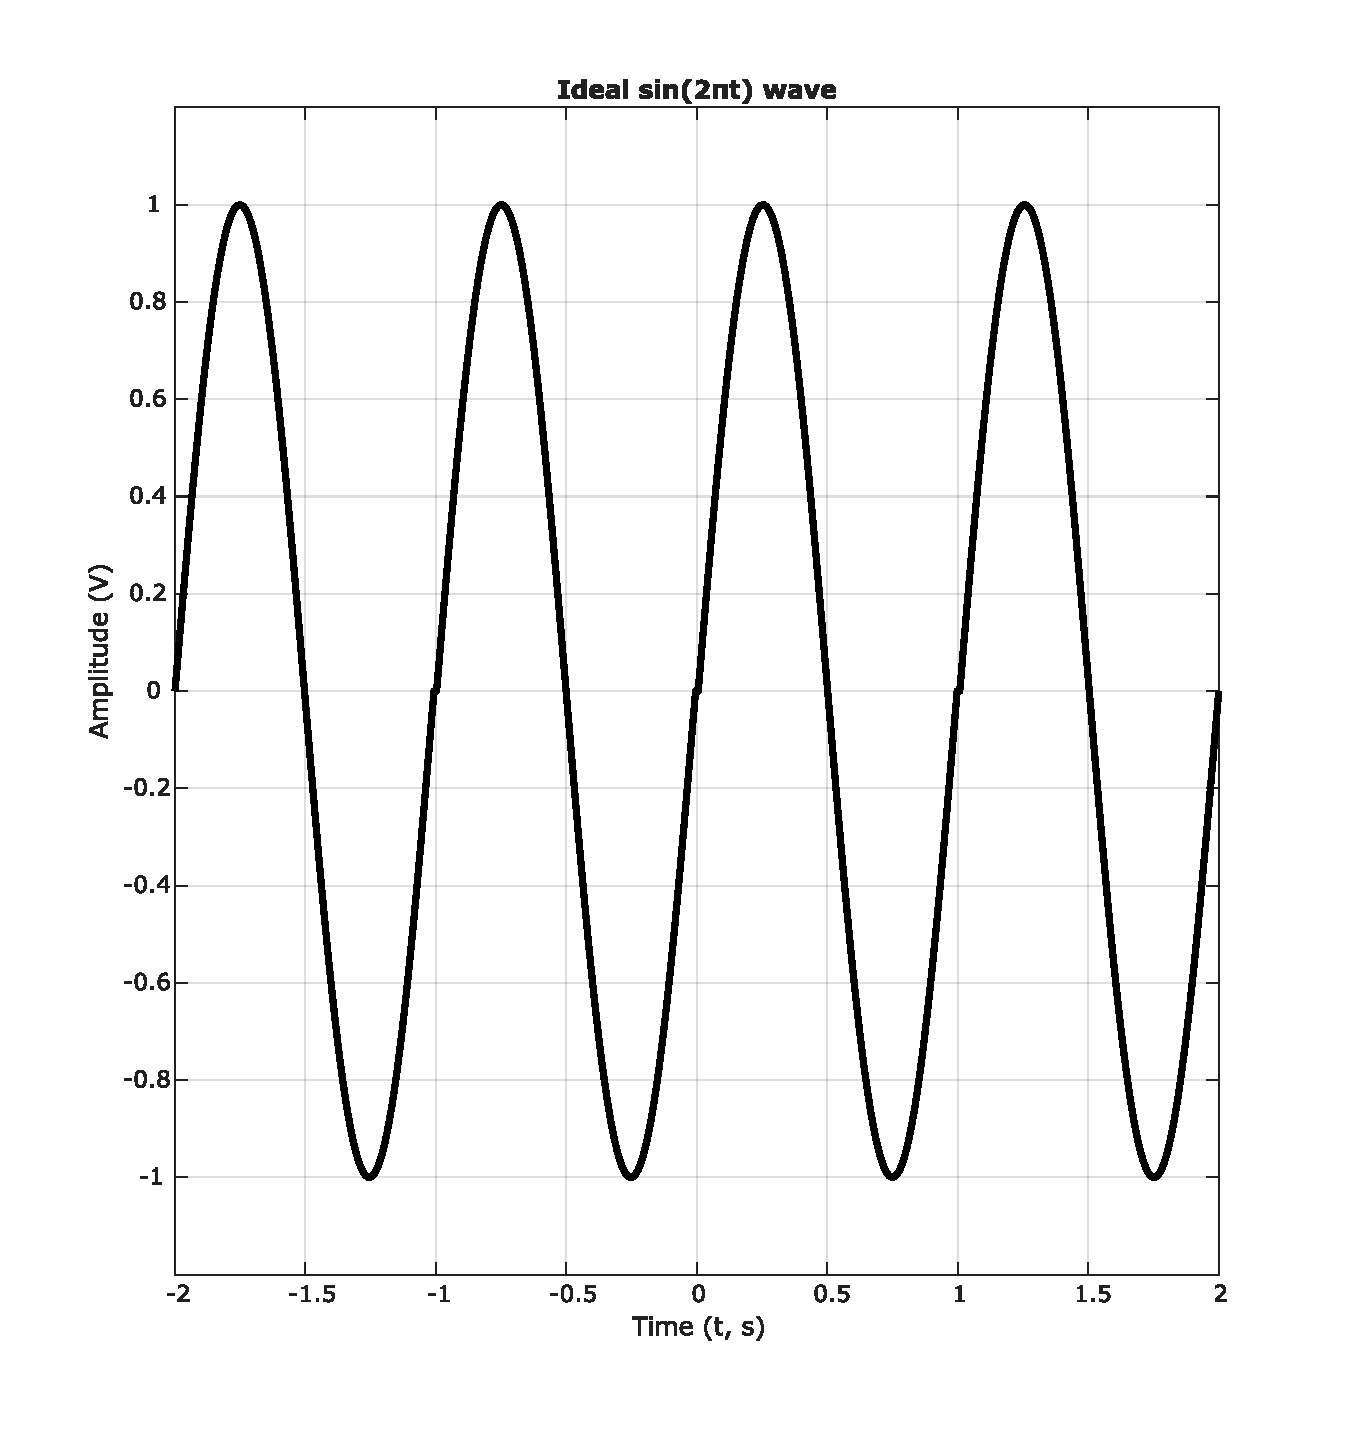
\includegraphics[width=10cm]{figures/SinWave_perfect_series.pdf}
\caption{The ideal representation of $\sin(2\pi t)$}
\label{fig:sinperfect}
\end{figure}

The first step in calculating the Fourier series is finding expressions for $a_n$ and $b_n$. However, by inspection it can be concluded that the function (\ref{eq:sine}) is odd, implying that (\ref{eq:andef}) will evaluate to zero for all values of $n$, and only an expression for $b_n$ is required. \\ 
Substituting the values from (\ref{eq:sine}) into (\ref{eq:bndef}) yields:
\begin{equation}
    \label{eqn:bn_sin}
    b_n = \frac{2}{1} \int_{0}^{1} \sin (2 \pi t) \sin (2 \pi n t) \, dt,
\end{equation}
which can be simplified using the following identities for the integral over exactly one period:

%\begin{align}
    \begin{equation}
        \int_{0}^{T} \sin (m t) \sin (n t) \, dt = 
        \left\{
            \begin{array}{lr}
                0,            & m \ne n\\
                \frac{1}{2}T, & m = n 
            \end{array}\nonumber
        \right. \ \ \ 
    \end{equation}
    
    \begin{equation}
        \int_{0}^{T} \cos (m t) \cos (n t) \, dt = 
        \left\{
            \begin{array}{lr}
                0,            & m \ne n\\
                \frac{1}{2}T, & m = n \nonumber
            \end{array}
        \right. \ \ \ 
    \end{equation}
    
    \begin{equation}
        \int_{0}^{T} \sin (m t) \cos(n t) \, dt = 0, \ \ \ \ \text{for } n,m \in \mathbb{R}\nonumber
    \end{equation}
%\end{align}
 to the following
\begin{equation}
    \label{eqn:bn_sin_fin}
    b_n = \frac{2}{1} \int_{0}^{T} \sin (2 \pi t) \sin (n 2 \pi t) \, dt = 
    \left\{
        \begin{array}{lr}
            \frac{2}{1} \times \frac{1}{2}T = T = 1,    & n = 1\\
            0, & n \ne 1 
        \end{array}
    \right.
\end{equation}
Equation (\ref{eqn:bn_sin_fin}) is true since $2\pi$ is only ever equal to $2\pi n$ when $n=1$.
From this it follows that $b_n = 1$ for $n=1$ and $b_n = 0$ for all other values of $n$.
\newline
Substituting $b_n$ and $a_n$ into equation (\ref{eq:fourierdef}): 
\begin{equation}
    \label{eq:fourier_sin_final}
    x(t) = \sin(2 \pi (1) t) = \sin(2 \pi t) = \cos(2\pi t - \frac{\pi}{2})
\end{equation}
Since the Fourier series of $x(t)$ is the exact same as the original equation $x(t)$. It can be safely inferred that there will only be one magnitude component and a constant for the phase component. 

Simulating this result with one component yields \textit{figure} \ref{fig:sinc1}. It is evident that the Fourier series expansion is the same as the original waveform function, however to further this point \textit{figures} \ref{fig:sinc2} to \ref{fig:sinc10} are generated. These figures show the expansion of $\sin(2\pi t)$ using two, five, and ten components.

\begin{figure}[H]
    \centering
    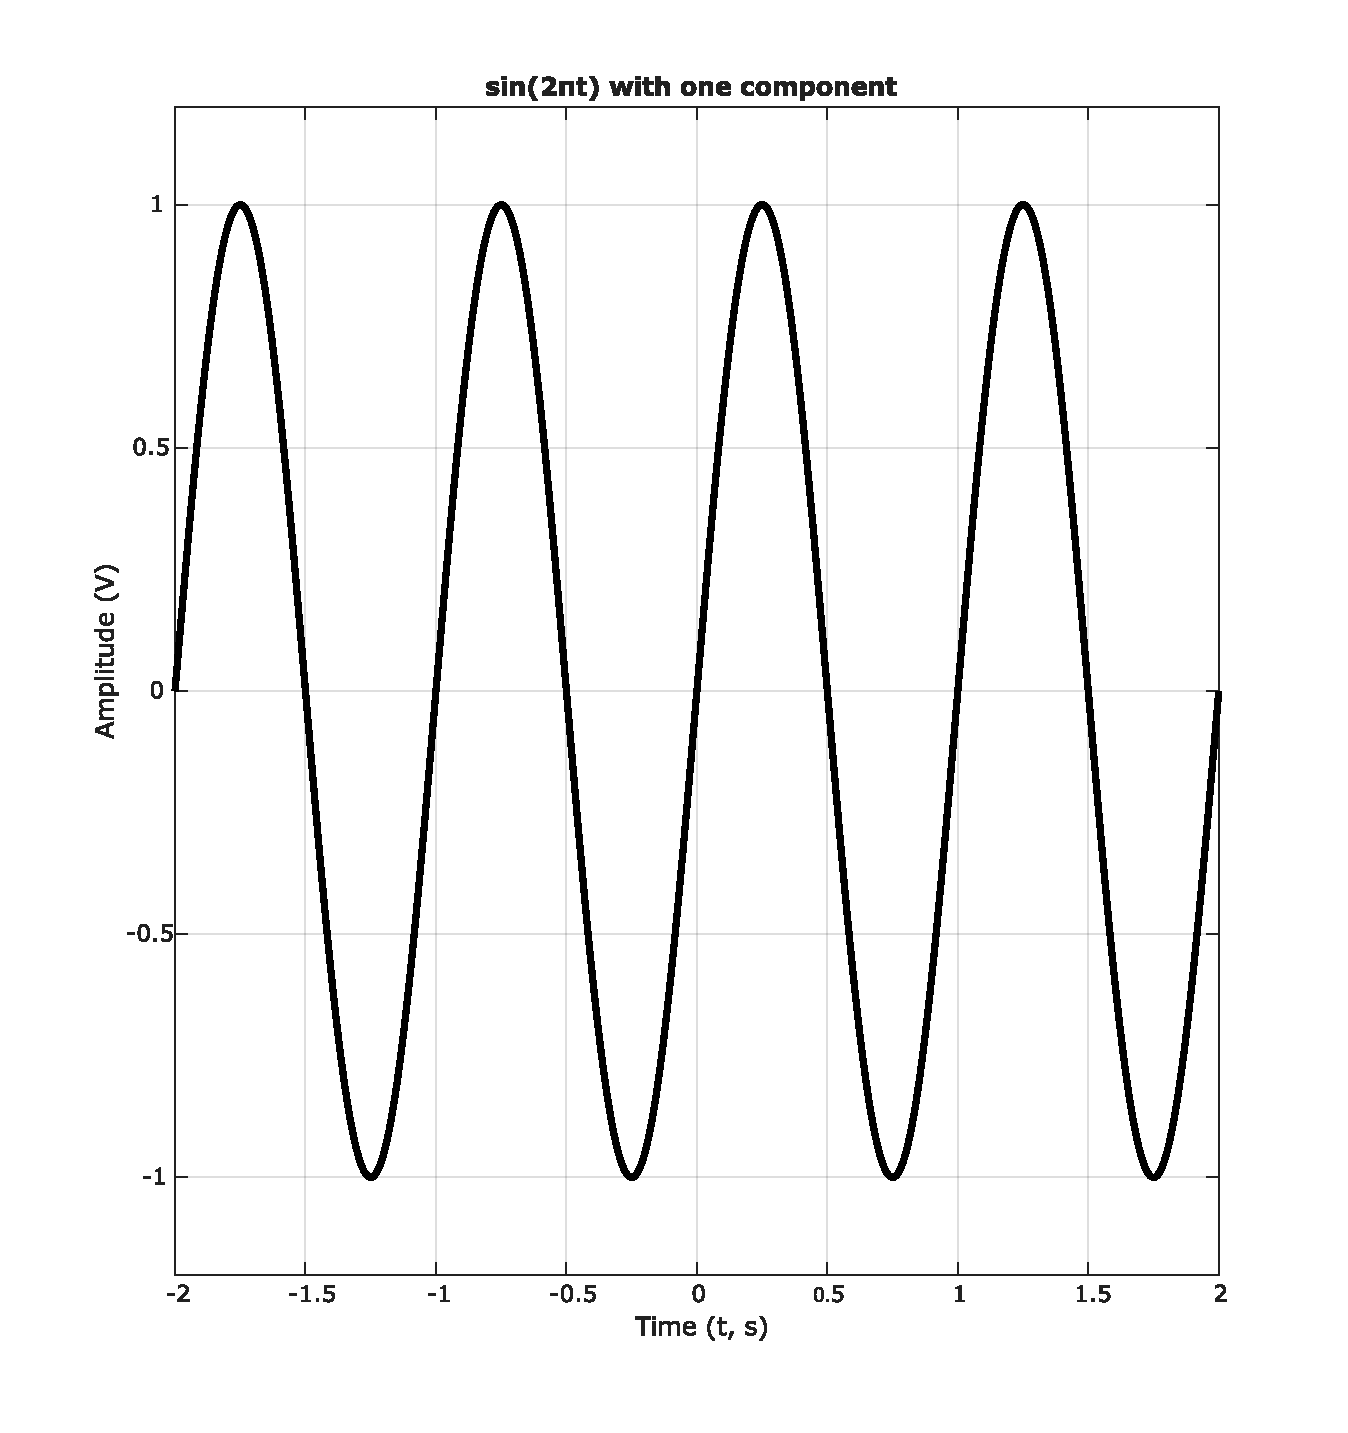
\includegraphics[width=10cm]{figures/SinWave_c1_series.pdf}
    \caption{Plot of the Fourier expansion for $\sin(2\pi t)$ using one component}
    \label{fig:sinc1}
\end{figure}

\begin{figure}[H]
    \centering
    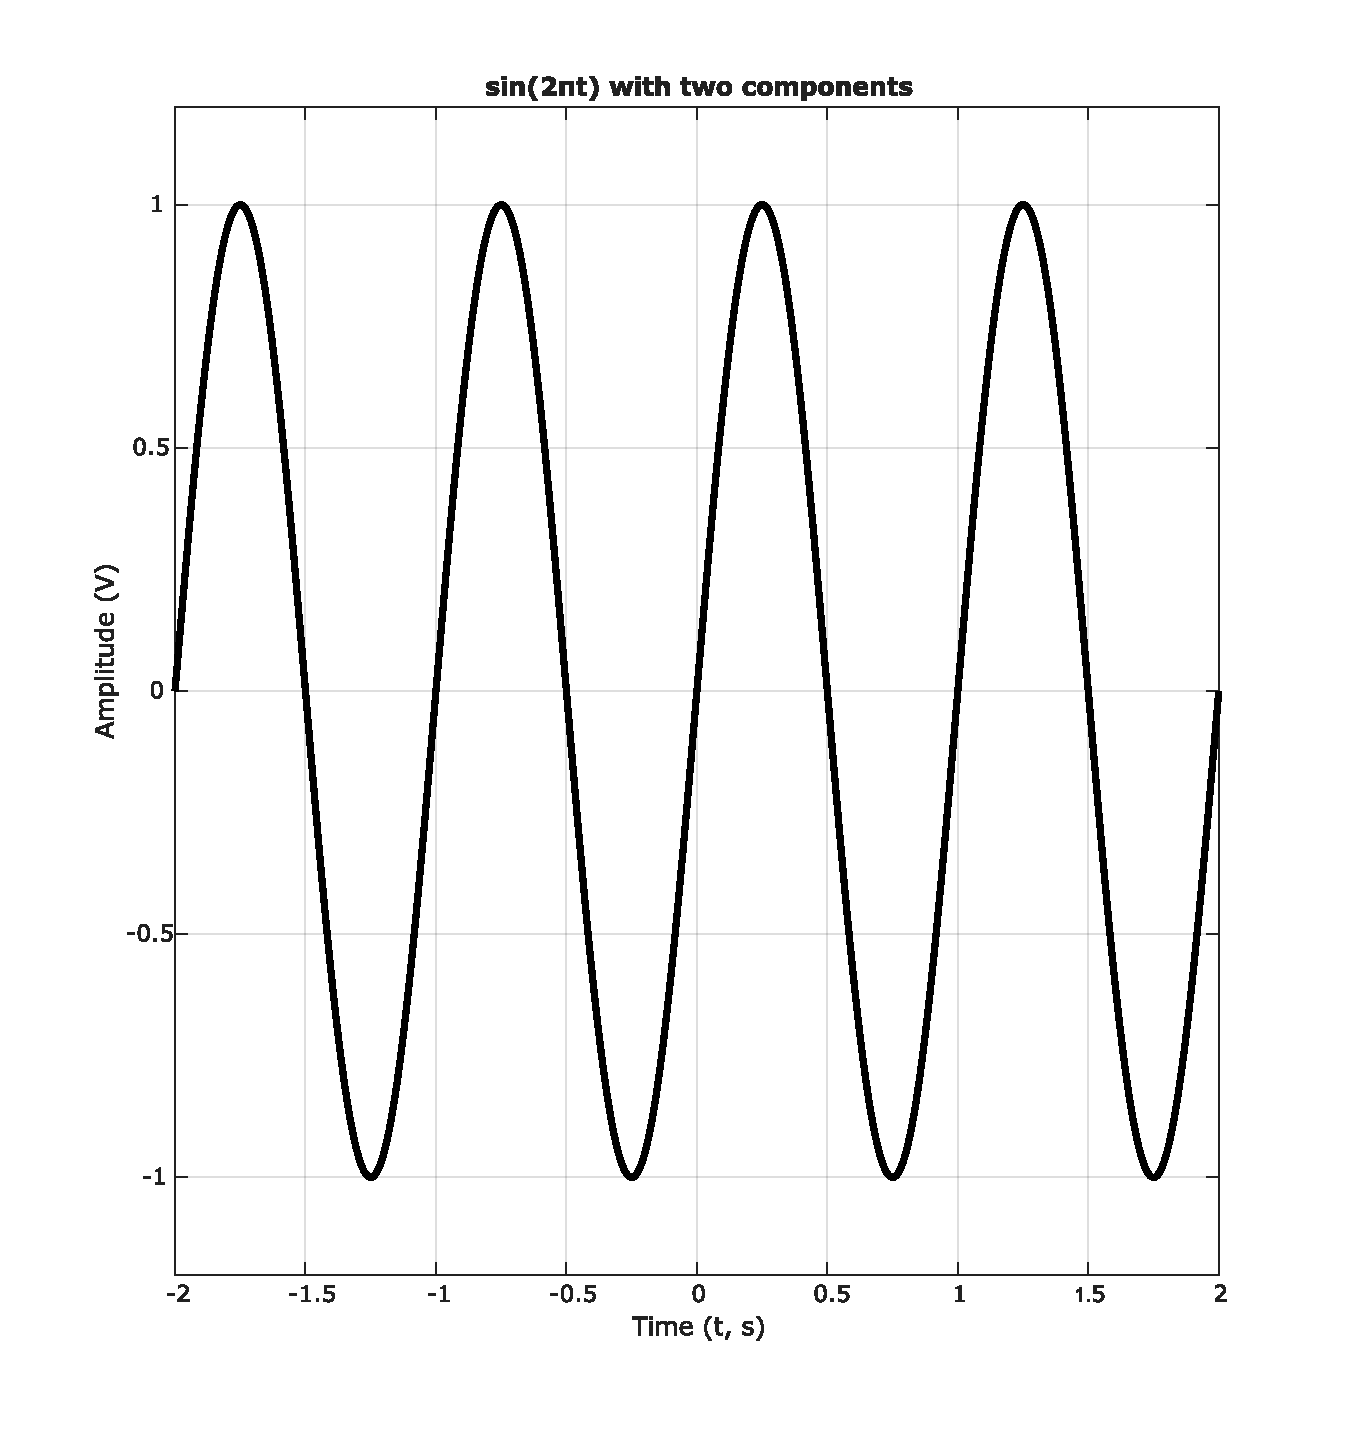
\includegraphics[width=10cm]{figures/SinWave_c2_series.pdf}
    \caption{Plot of $\sin(2\pi t)$ using two components}
    \label{fig:sinc2}
\end{figure}

\begin{figure}[H]
    \centering
    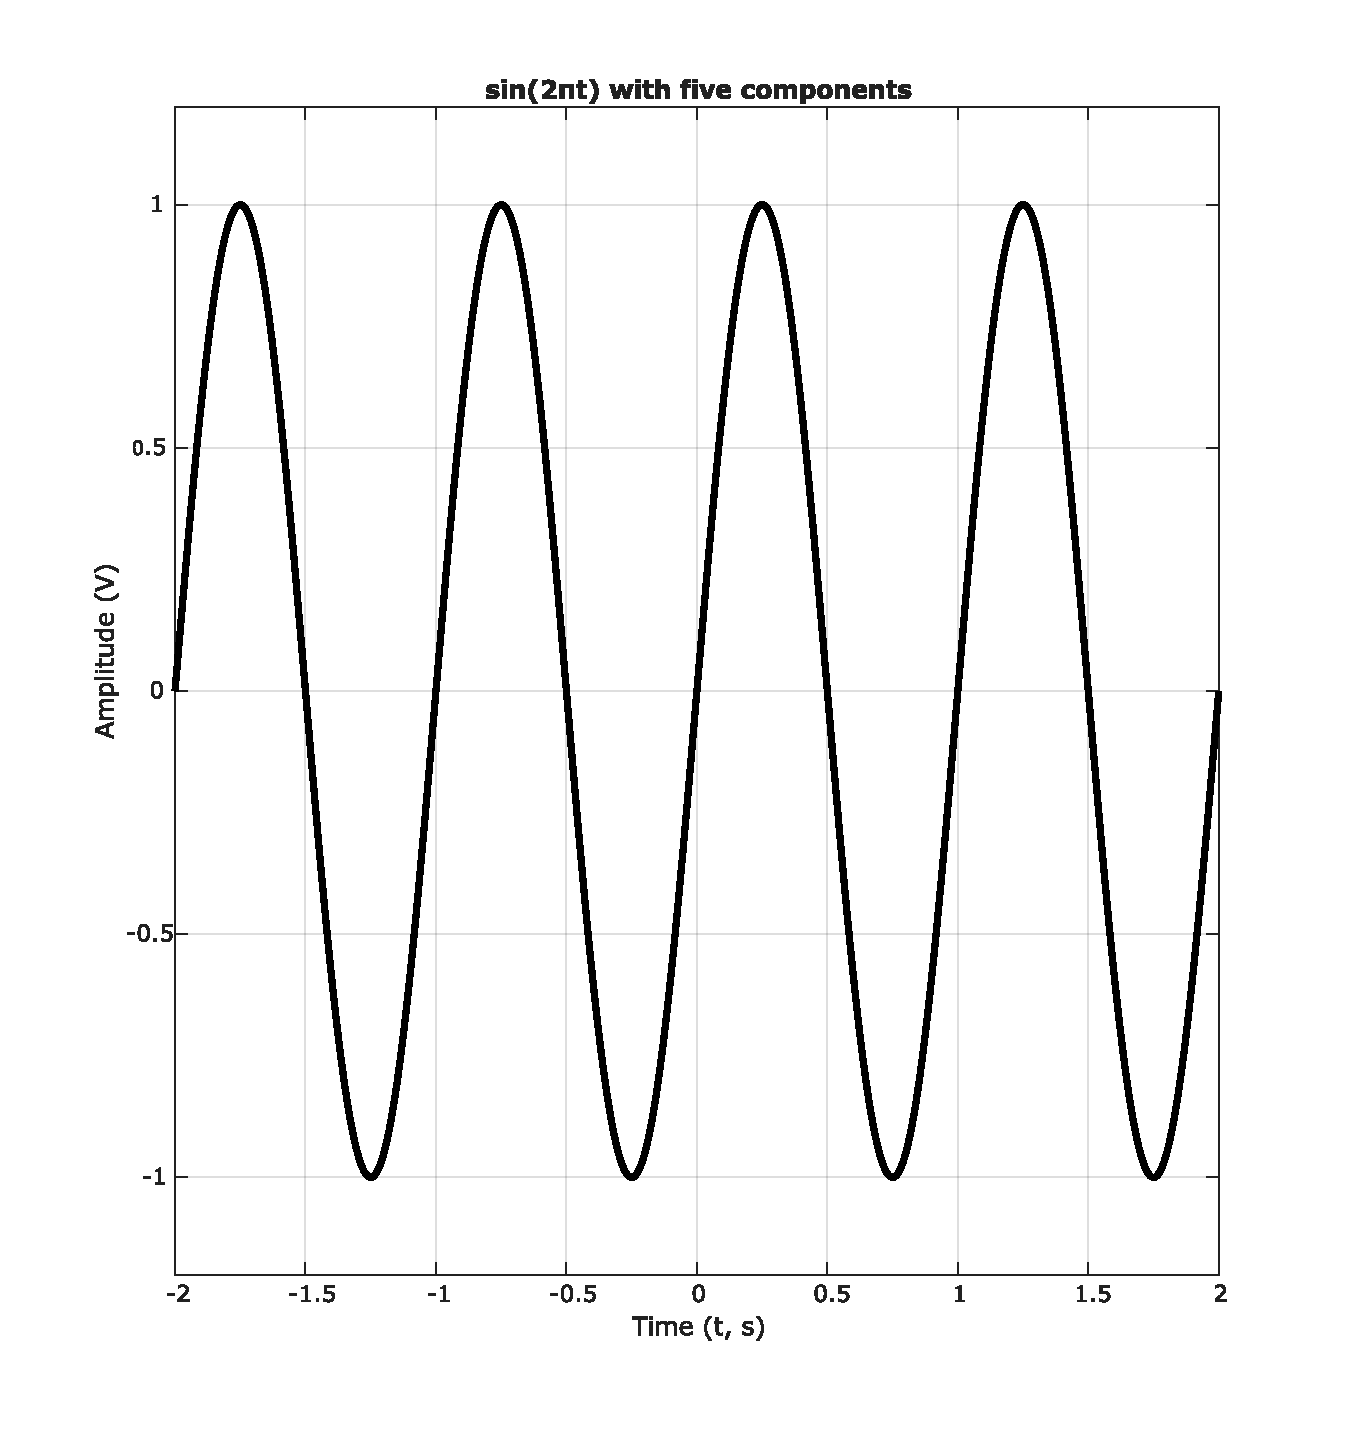
\includegraphics[width=10cm]{figures/SinWave_c5_series.pdf}
    \caption{$\sin(2\pi t)$ plotted with five components}
    \label{fig:sinc5}
\end{figure}

\begin{figure}[H]
    \centering
    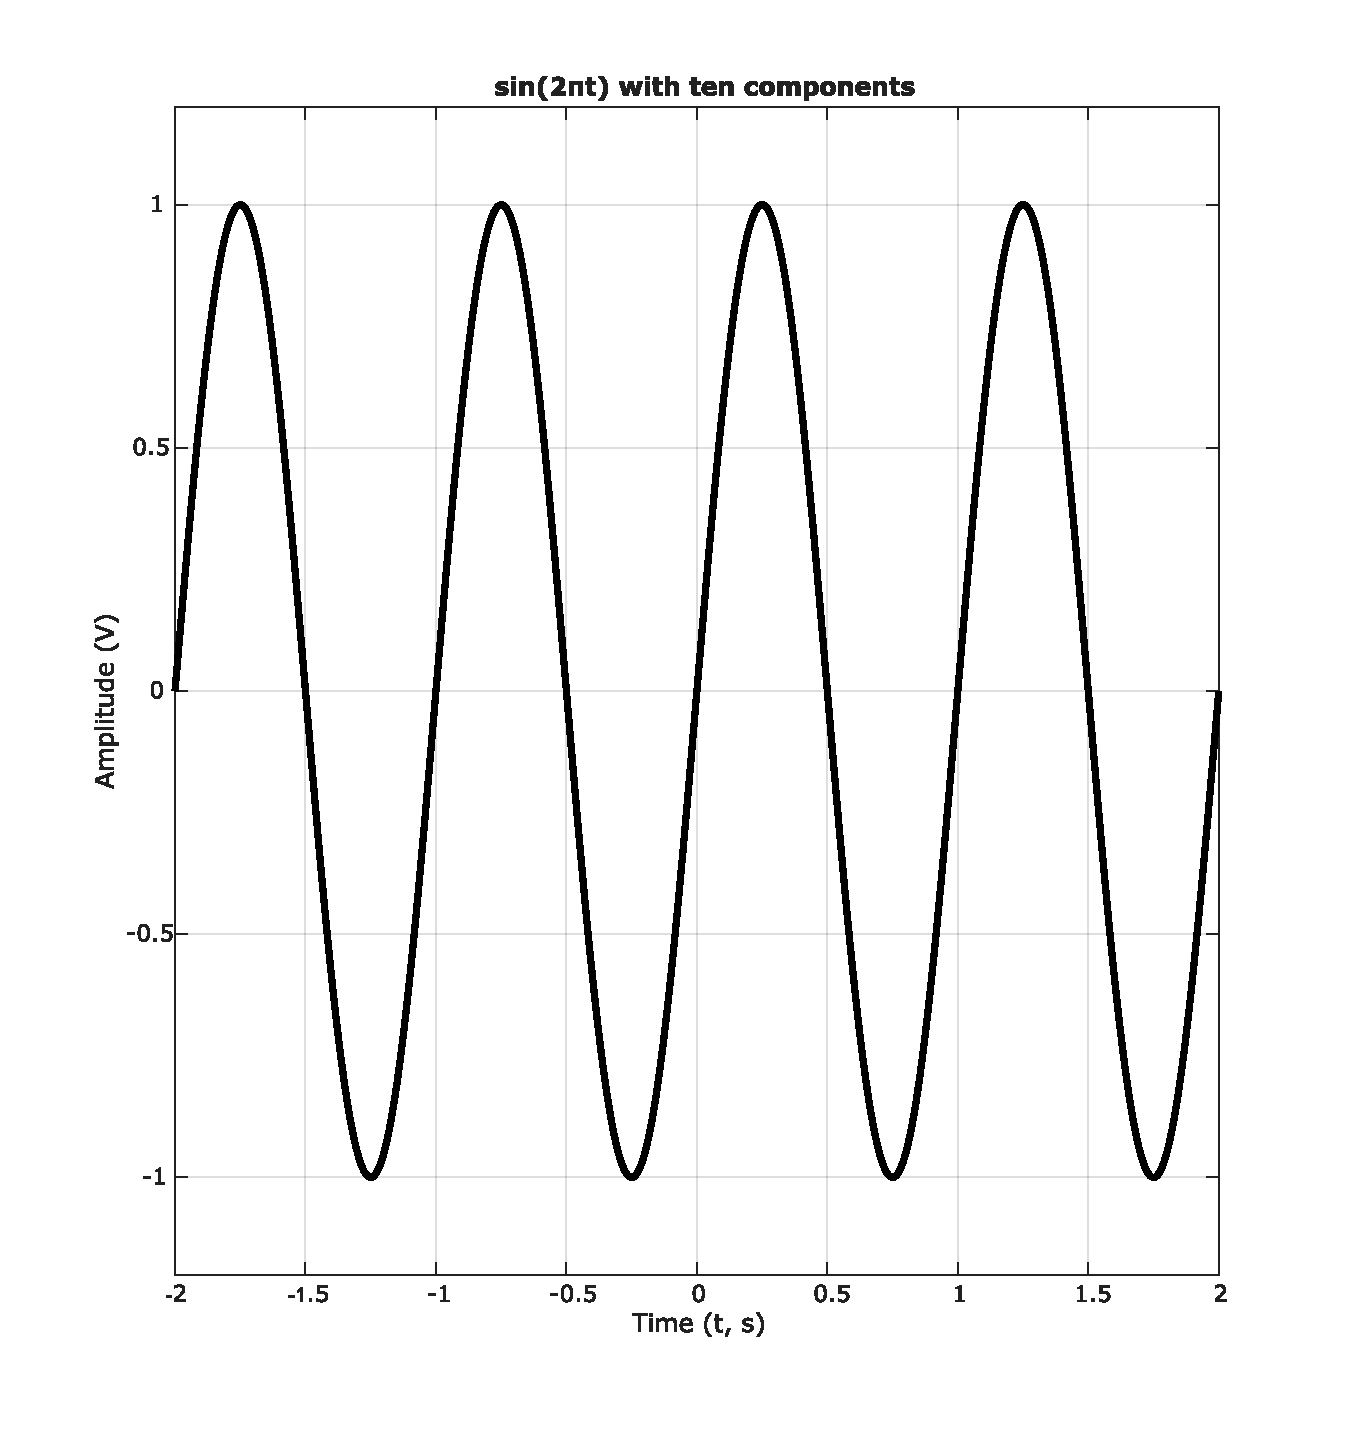
\includegraphics[width=10cm]{figures/SinWave_c10_series.pdf}
    \caption{Fourier series expansion of $\sin(2\pi t)$ with ten components}
    \label{fig:sinc10}
\end{figure}

It is clear that no difference is made when using varying amounts of components in the Fourier expansion. This is due to the fact that $\sin(2\pi t)$ is already a smooth sinusoidal waveform. As such, it is redundant to apply the Fourier series to this waveform and no further information can be gained by doing so, as shown by the FFT (Fast Fourier Transform), and magnitude and phase spectra in \textit{figures} \ref{fig:sin_mag} to \ref{fig:sinFFT}.

\begin{figure}[H]
    \centering
    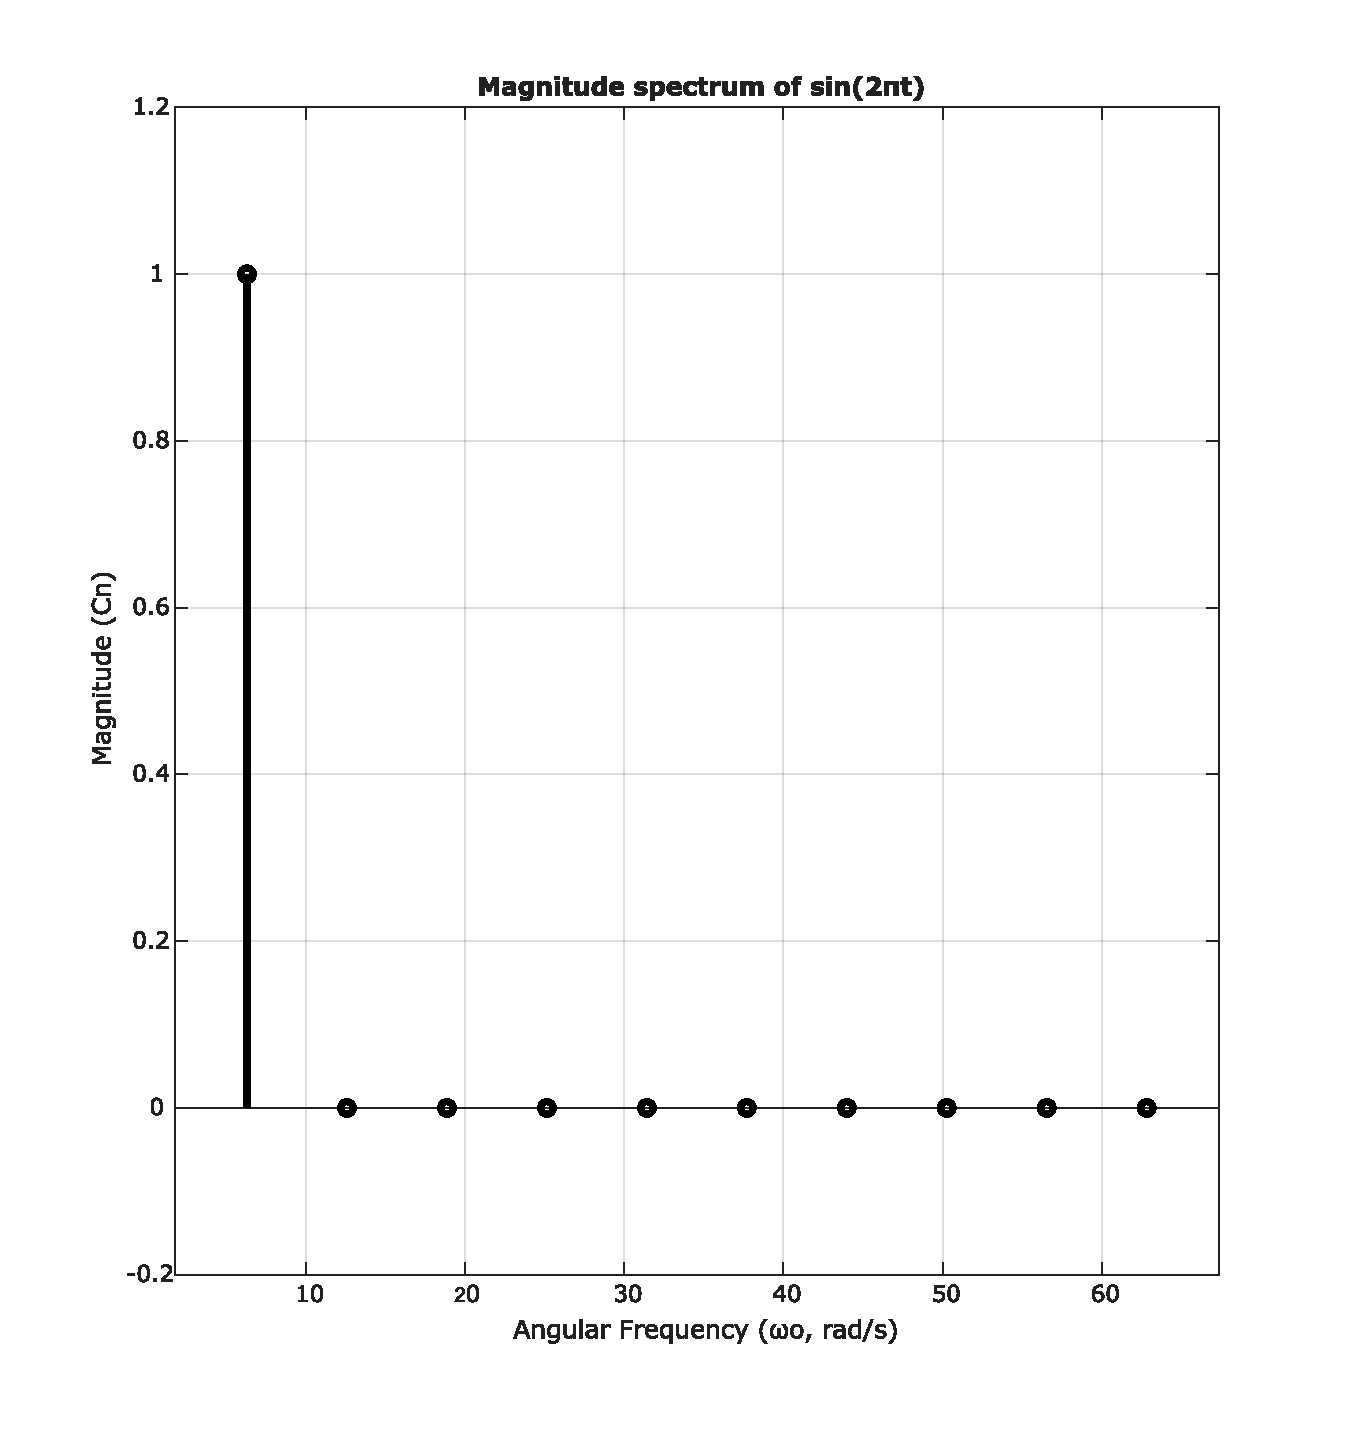
\includegraphics[width=10cm]{figures/SinWave_c10_magnitude_spectra.pdf}
    \caption{Magnitude spectra of $\sin(2\pi t)$ with ten components}
    \label{fig:sin_mag}
\end{figure}

\begin{figure}[H]
\label{fig:sin_phase}
\centering
    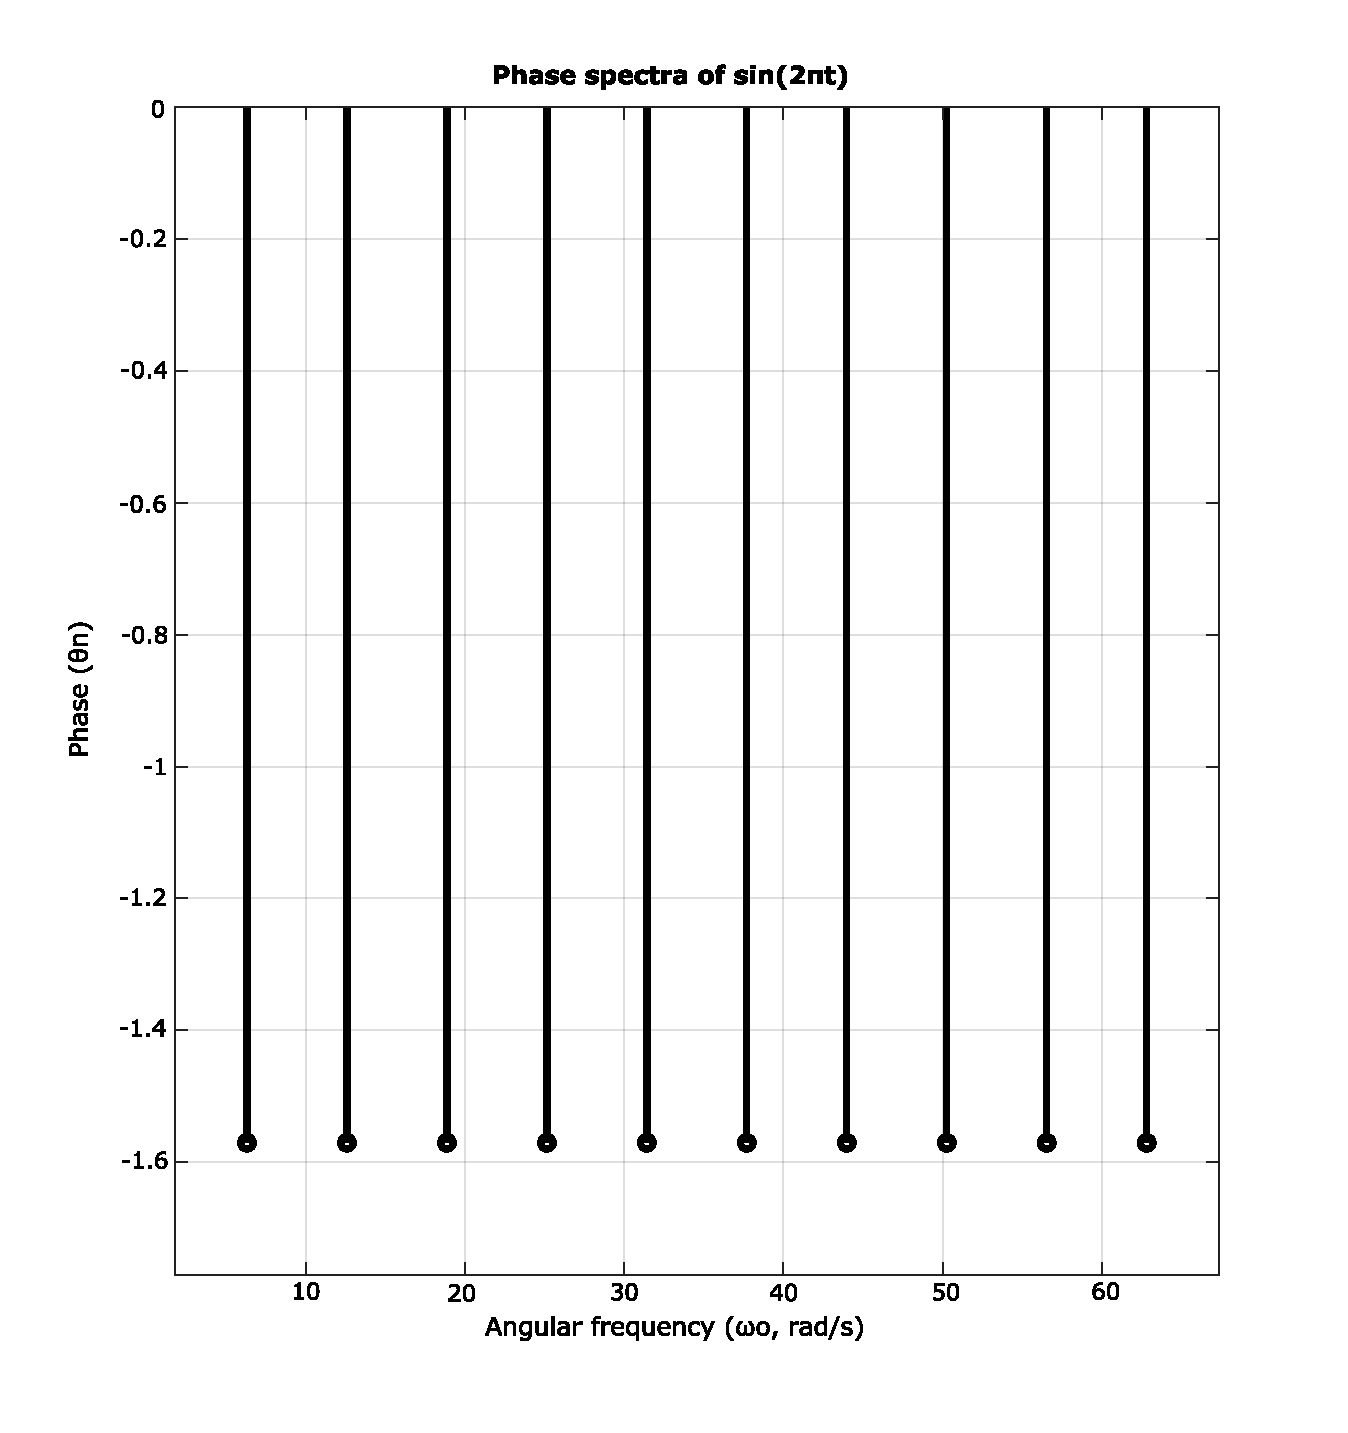
\includegraphics[width=10cm]{figures/SinWave_c10_phase_spectra.pdf} % sin phase
    \caption{Phase spectra for $\sin(2\pi t)$ with ten components}
\end{figure}

\begin{figure}[H]
    \centering
    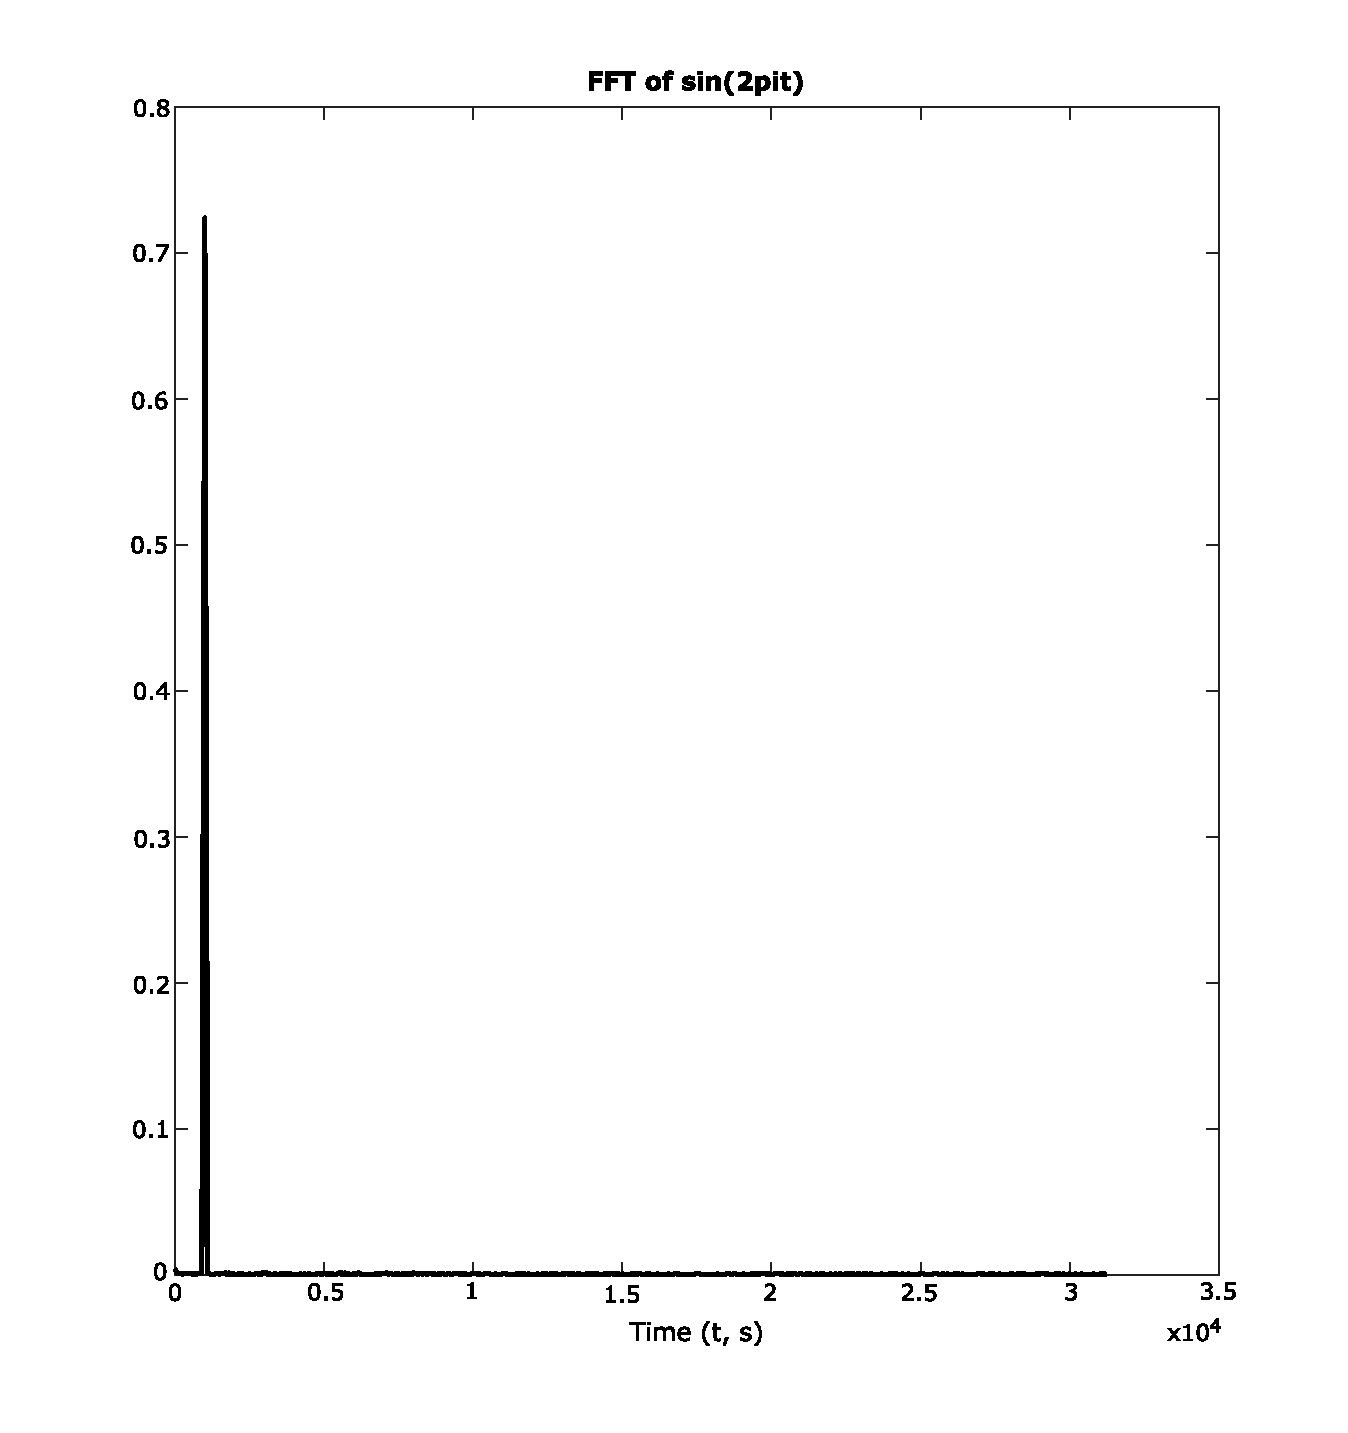
\includegraphics[width=10cm]{figures/Sin_TEK_plot.pdf}
    \caption{FFT of $\sin(2\pi t)$}
    \label{fig:sinFFT}
\end{figure}


\subsection{Square wave with a 50\% duty cycle}
\label{sec:square50}

The way a square wave is defined is similar to a unit-step function where for a portion of the period, it is active (i.e. equal to 1), and the rest is inactive (equal to -1 or 0). In this case half is active, while the other half is inactive. This is mathematically expressed as
\begin{align}
    x(t) &= \begin{cases}
    1, & \text{if } 0 \leq t < 0.5 \\
   -1, & \text{if } 0.5 \leq t < 1,
   \end{cases} 
\end{align}
with $T = 1$ and $\omega_0 = 2\pi$. Once again the function is odd, since it satisfies
\begin{equation}
    f(-t) = -f(t)
\end{equation}
and $a_n$ is zero for all $n$. The only required coefficient is thus $b_n$ and only $\sin$-terms will remain in the final expression.\\
From (\ref{eq:bndef}), $b_n$ becomes
\begin{align}
    b_n &= \frac{2}{1} \left[ \int_{0}^{0.5} x(t) \sin \left( \frac{2\pi n t}{1} \right) \, dt
- \int_{0.5}^{1} \sin \left( \frac{2\pi n t}{1} \right) \, dt \right] \nonumber\\
\end{align}
After evaluating the integral the result is:
\begin{align}
 &= 2 \left[ \frac{-1}{2 \pi n t} (\cos (2 \pi n t)) \bigg|_0^{0.5} - \frac{1}{2 \pi n} (\cos (2 \pi n t)) \bigg|_{0.5}^{1} \right] \nonumber\\
 &= \frac{-1}{\pi n} \cos (\pi n) + \frac{1}{\pi n} + \frac{1}{2 \pi n} \cos (2 \pi n) - \frac{1}{2 \pi n} \cos (\pi n)\nonumber\\
 &= \frac{3}{2 \pi n} (1 - \cos (\pi n)), \nonumber \\
\end{align}
which equates to
\begin{align}
    b_n &= \begin{cases}
    \frac{3}{\pi n}, &\text{if $n$ is odd } \\
    0, &\text{if $n$ is even}.
\end{cases}
\end{align}
The full Fourier expansion of the signal then becomes
\begin{equation}
\label{eq:square50_fourier}
    x(t) = \sum_{odd\; n}^{\infty}\frac{3}{\pi n} \sin (n 2 \pi t),
\end{equation}
after which, using (\ref{eq:compactfourier}) to (\ref{eq:Cn}), the compact form can be expressed as
\begin{equation}
    x(t)= \sum_{odd\;n}^{\infty}\frac{3}{\pi n} \cos \left(2 \pi n t - \frac{\pi}{2}\right).
\end{equation}

\textit{Figure} \ref{fig:square50_perf} shows a perfect plot of the square wave. Simulating (\ref{eq:square50_fourier}) using one component yields \textit{figure} \ref{fig:square50_c1}.

\begin{figure}[h]
\centering
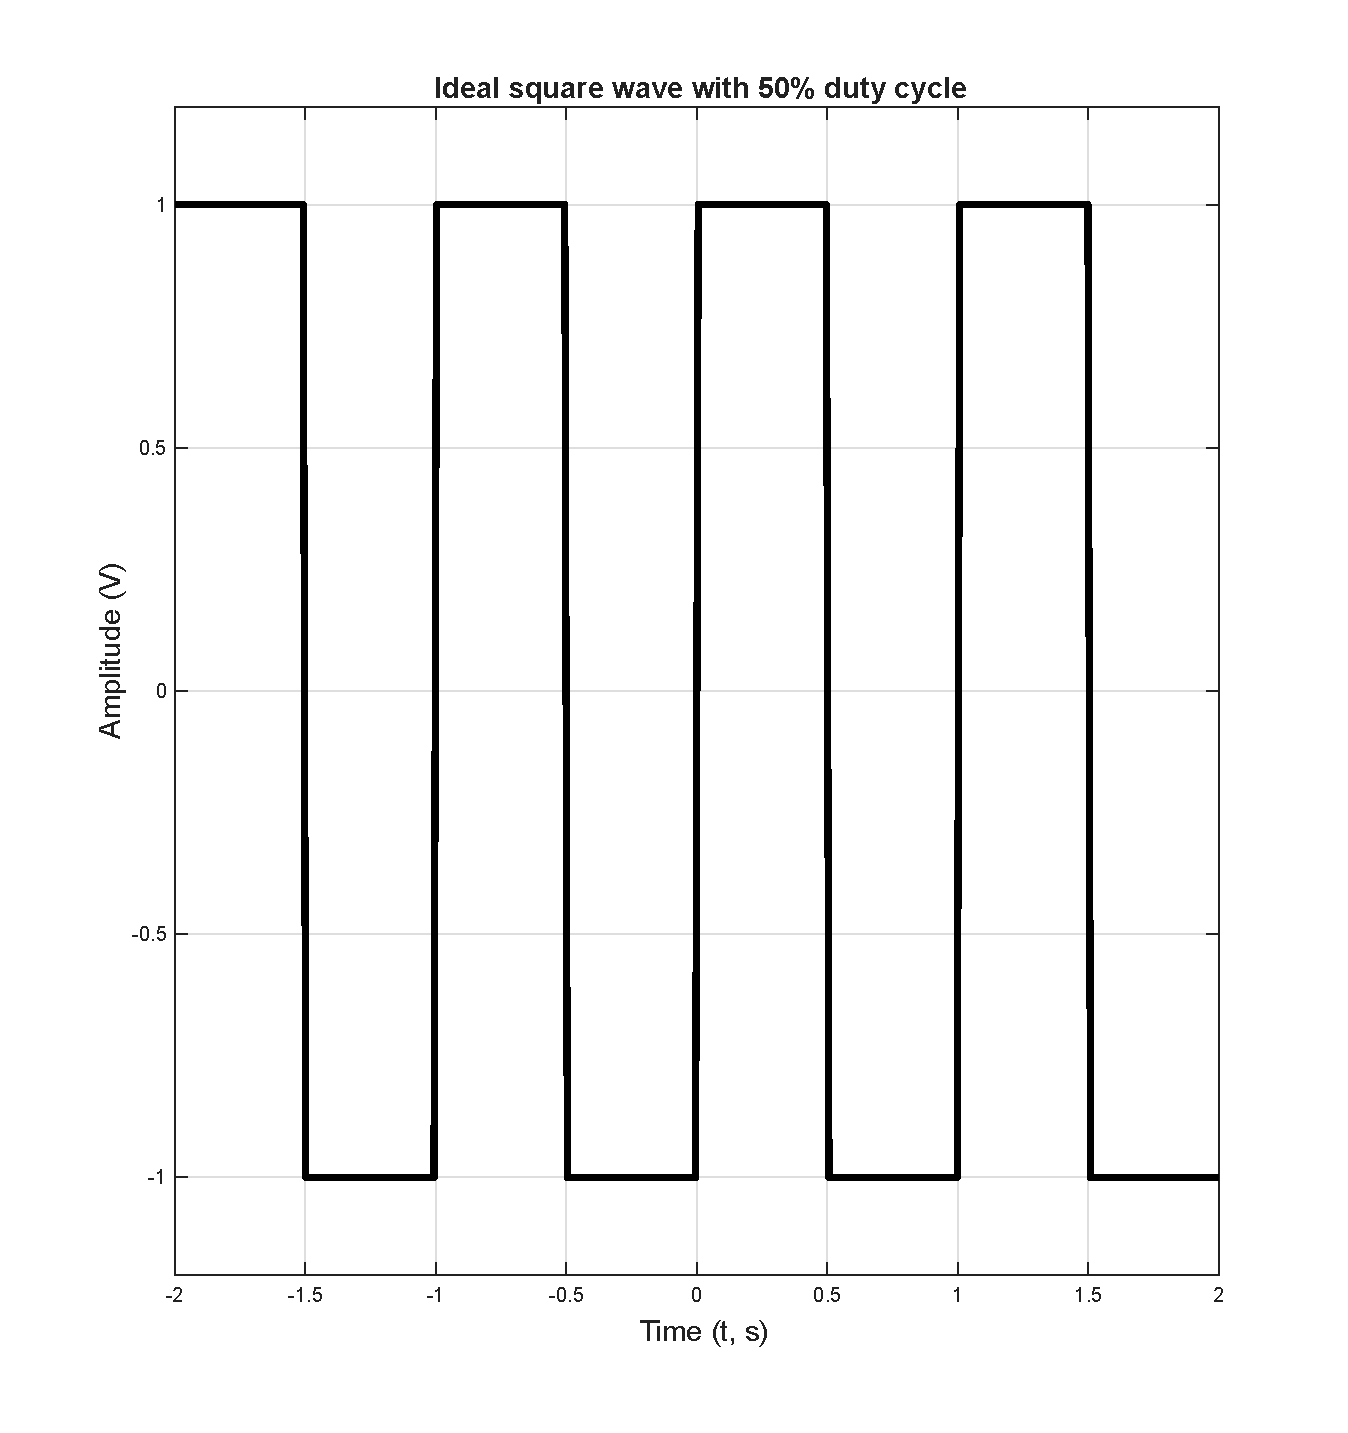
\includegraphics[width=10cm]{figures/SquareWave_50_perfect_series.pdf} %sq50 perf
\caption{Ideal waveform of a square wave with a 50\% duty cycle}
\label{fig:square50_perf}
\end{figure}

\begin{figure}[H]
    \centering
    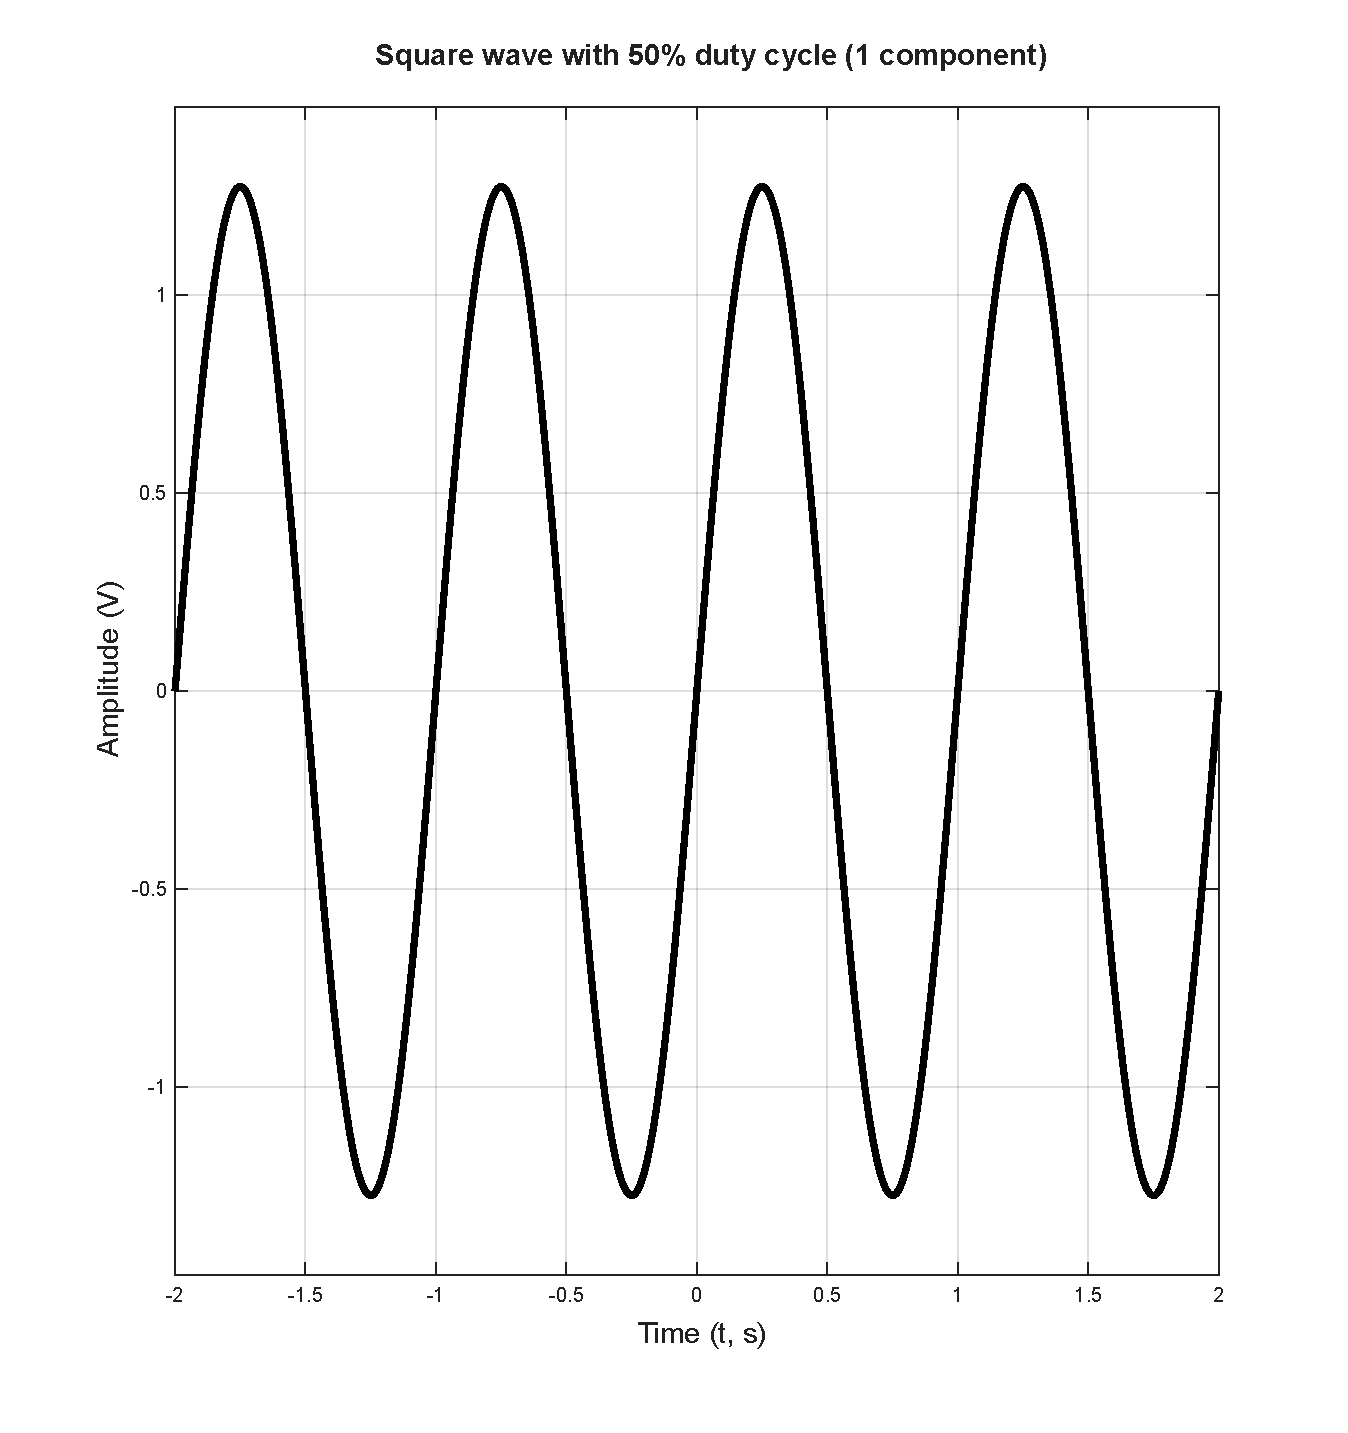
\includegraphics[width=10cm]{figures/SquareWave_50_c1_series.pdf}
    \caption{Fourier series of the 50\% duty cycle square wave with one component}
    \label{fig:square50_c1}
\end{figure}

The square wave in \textit{figure} \ref{fig:square50_c1} looks like a simple sine-wave, much like that seen in the previous section. This is to be expected when considering the form of equation (\ref{eq:square50_fourier}) in this case. In \textit{figure} \ref{fig:square50_c5}, the waveform already starts to look more like the ideal with only five components.

\begin{figure}[H]
    \centering
    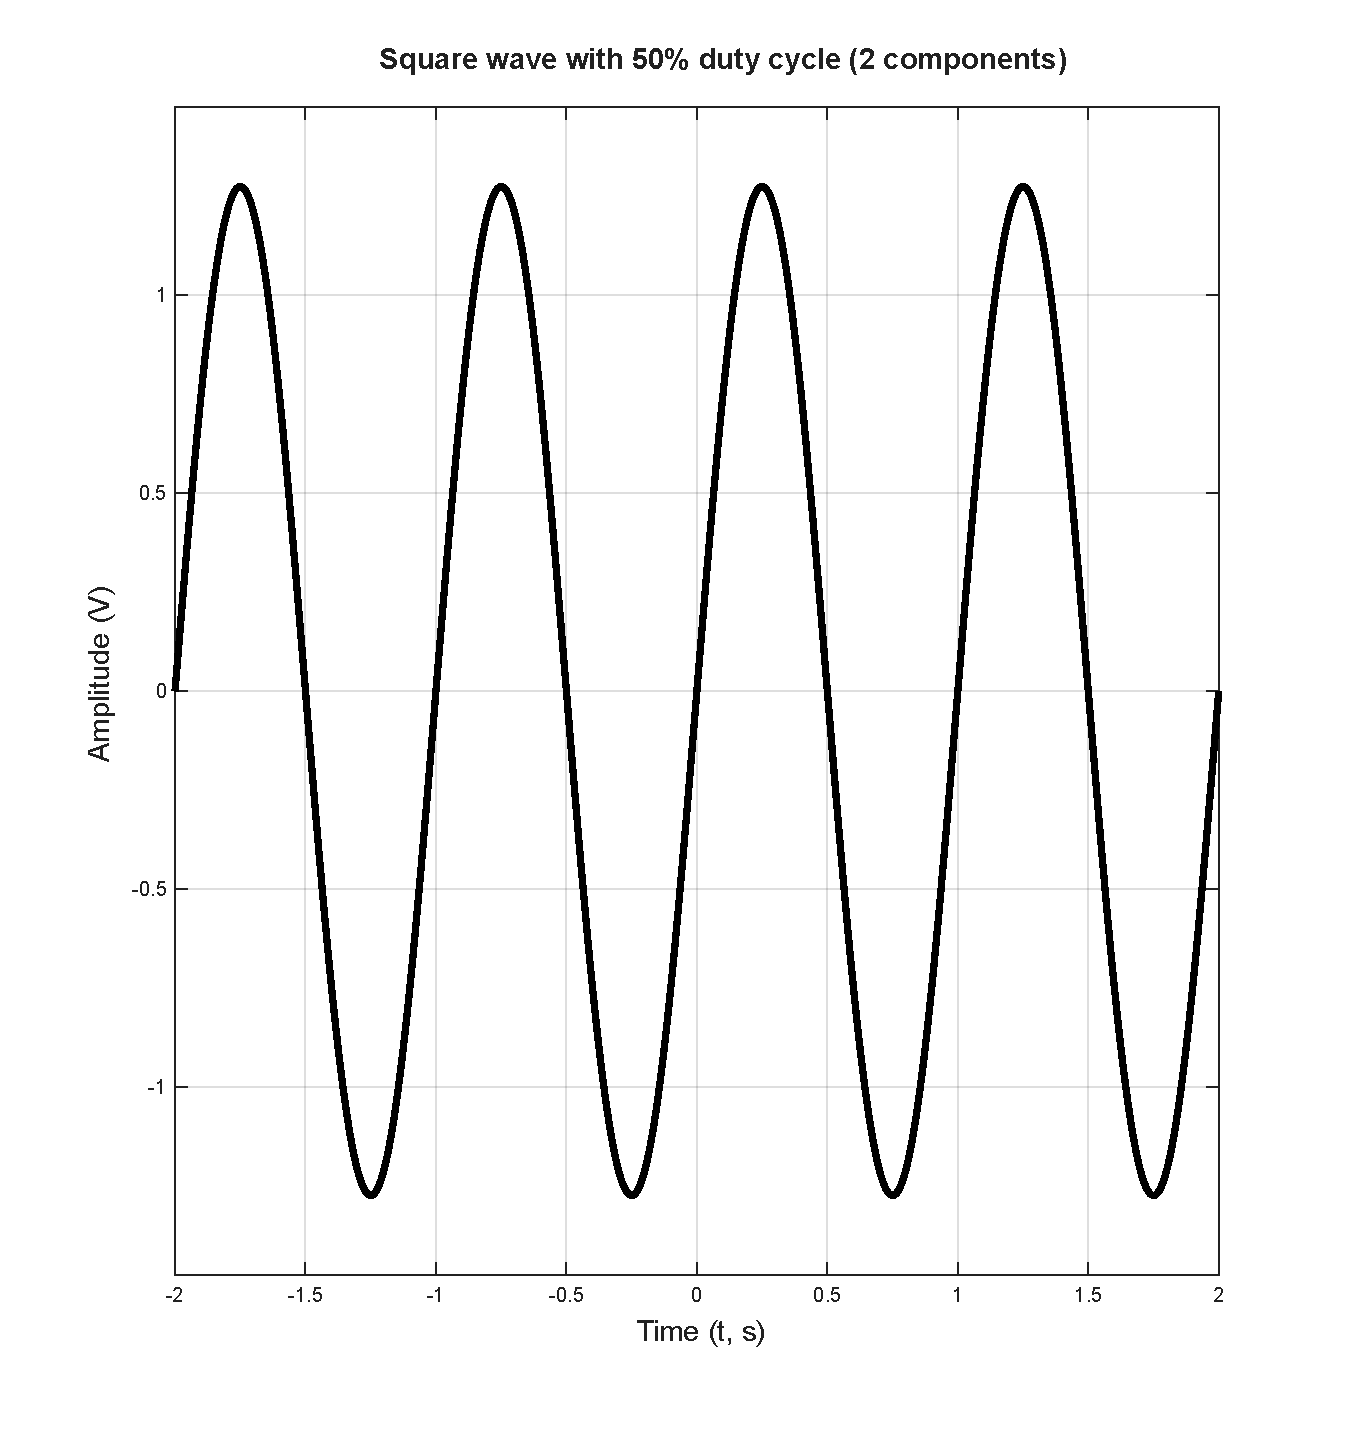
\includegraphics[width=10cm]{figures/SquareWave_50_c2_series.pdf}
    \caption{The 50\% duty cycle square wave with two components in the Fourier series}
    \label{fig:square50_c2}
\end{figure}

\begin{figure}[H]
    \centering
    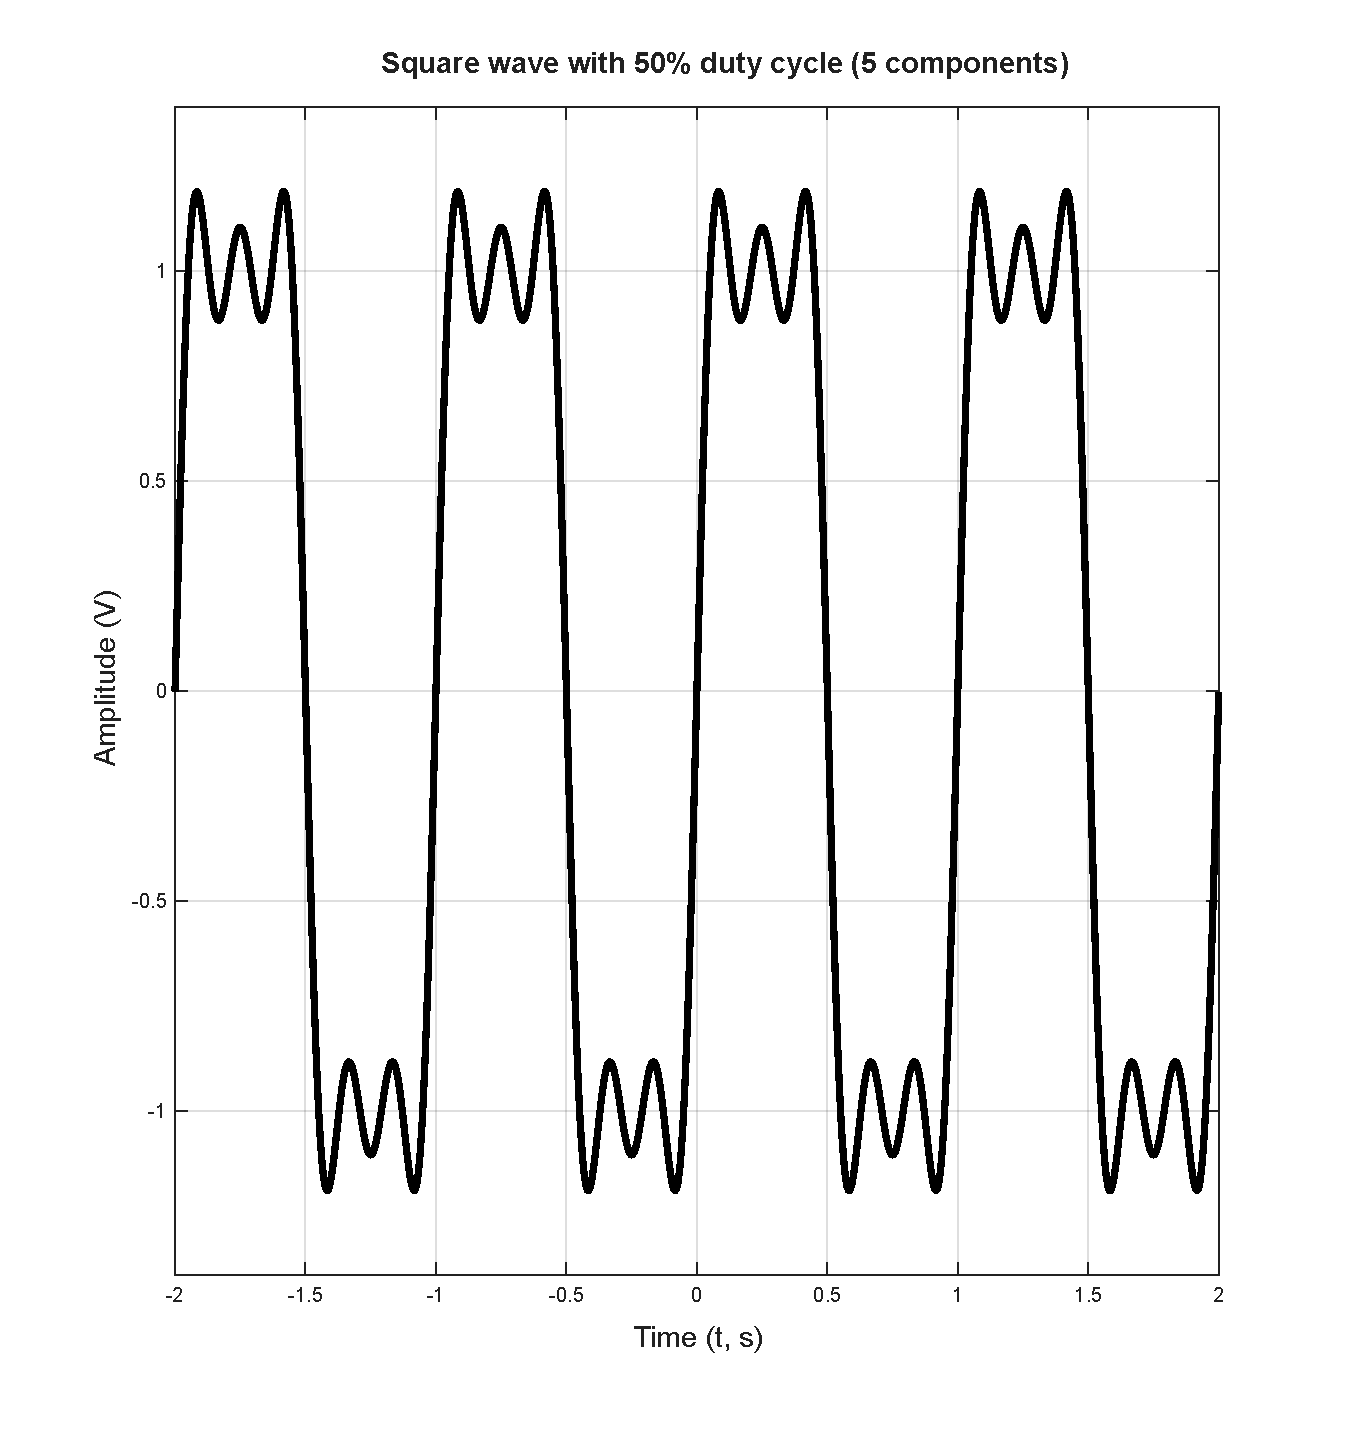
\includegraphics[width=10cm]{figures/SquareWave_50_c5_series.pdf}
    \caption{Fourier expansion of the 50\% duty cycle square wave with five components}
    \label{fig:square50_c5}
\end{figure}

\begin{figure}[h]
    \centering
    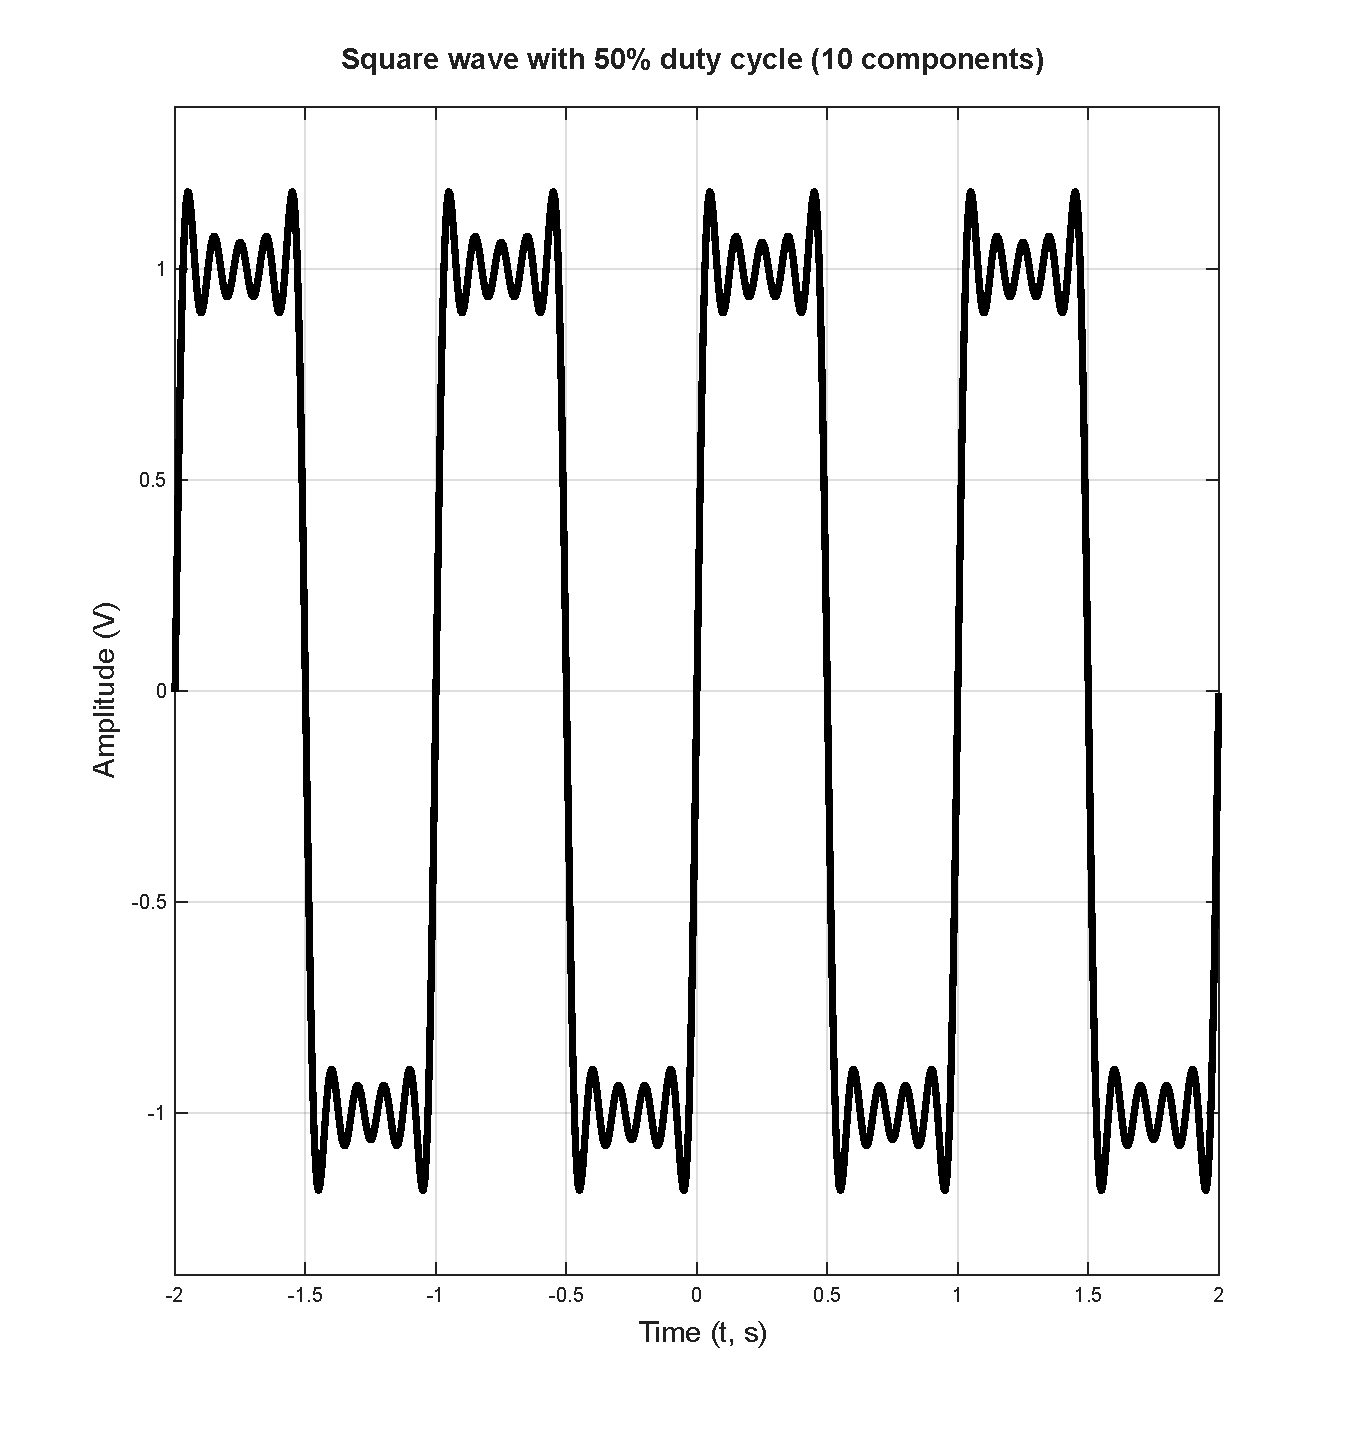
\includegraphics[width=10cm]{figures/SquareWave_50_c10_series.pdf}
    \caption{The Fourier expansion of the 50\% duty cycle square wave with ten components}
    \label{fig:square50_c10}
\end{figure}

It is clear that with more components of varying amplitudes and frequencies, the approximation of a waveform increases in accuracy, shown in \textit{figures} \ref{fig:square50_c5} to \ref{fig:square50_c10}. However, a caveat of the Fourier series also becomes clear. For discontinuous functions, a diversion of approximately 9\% appears around the point of discontinuity. This is known as the Gibbs phenomenon \cite{eli}. This phenomenon never truly disappears with more components added to the Fourier expansion, but reaches a sharper peak, eventually becoming almost invisible. This phenomenon is not a cause for concern though, as this very slight diversion is negligible for most applications.

The Fourier series still shows its efficacy in approximating a waveform as displayed in \textit{figures} \ref{fig:square50_FFT} to \ref{fig:square50_phase}. In the FFT, magnitude spectra and phase spectra, information usually tedious to find, is easily read. 

Note that the simulations for this and the previous waveform were conducted using MATLAB. The script is provided in Appendix \ref{app:code}.

\begin{figure}[H]
    \centering
    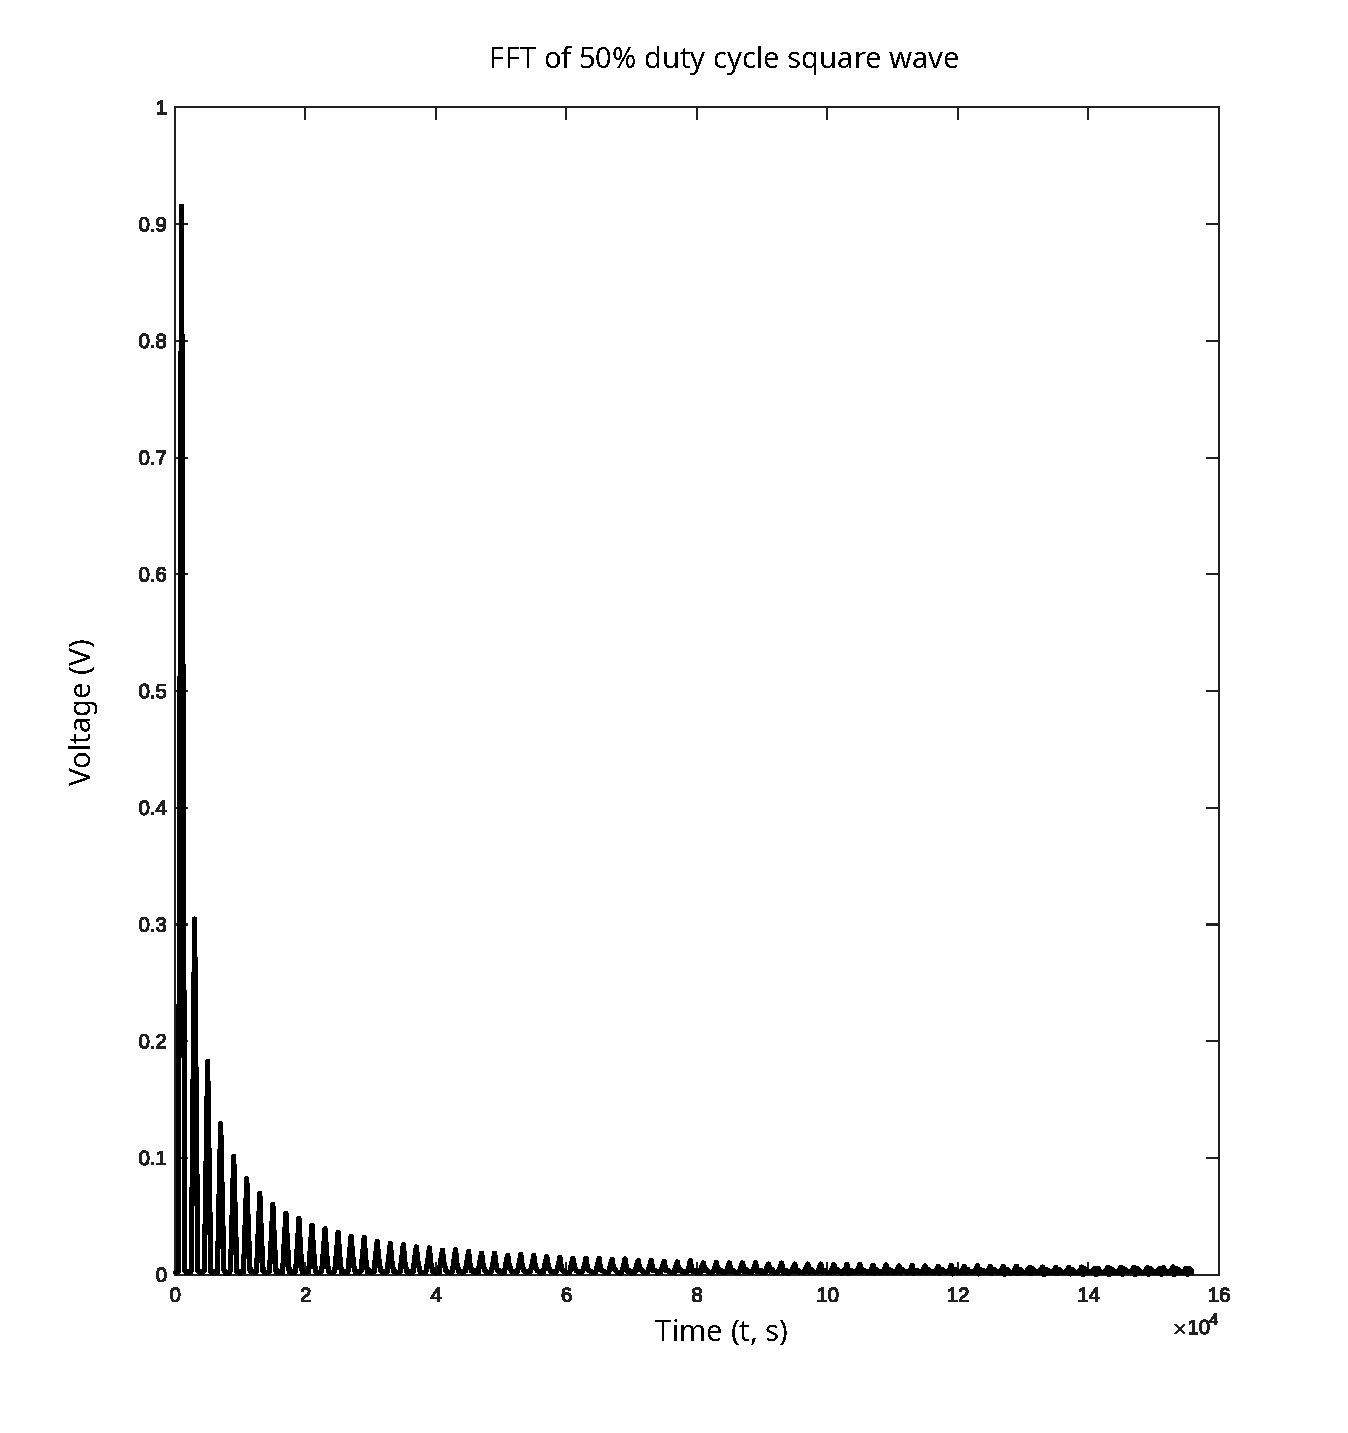
\includegraphics[width=10cm]{figures/Square_50_TEK_plot.pdf}
    \caption{FFT of the 50\% duty cycle square wave}
    \label{fig:square50_FFT}
\end{figure}

\begin{figure}[H]
    \centering
    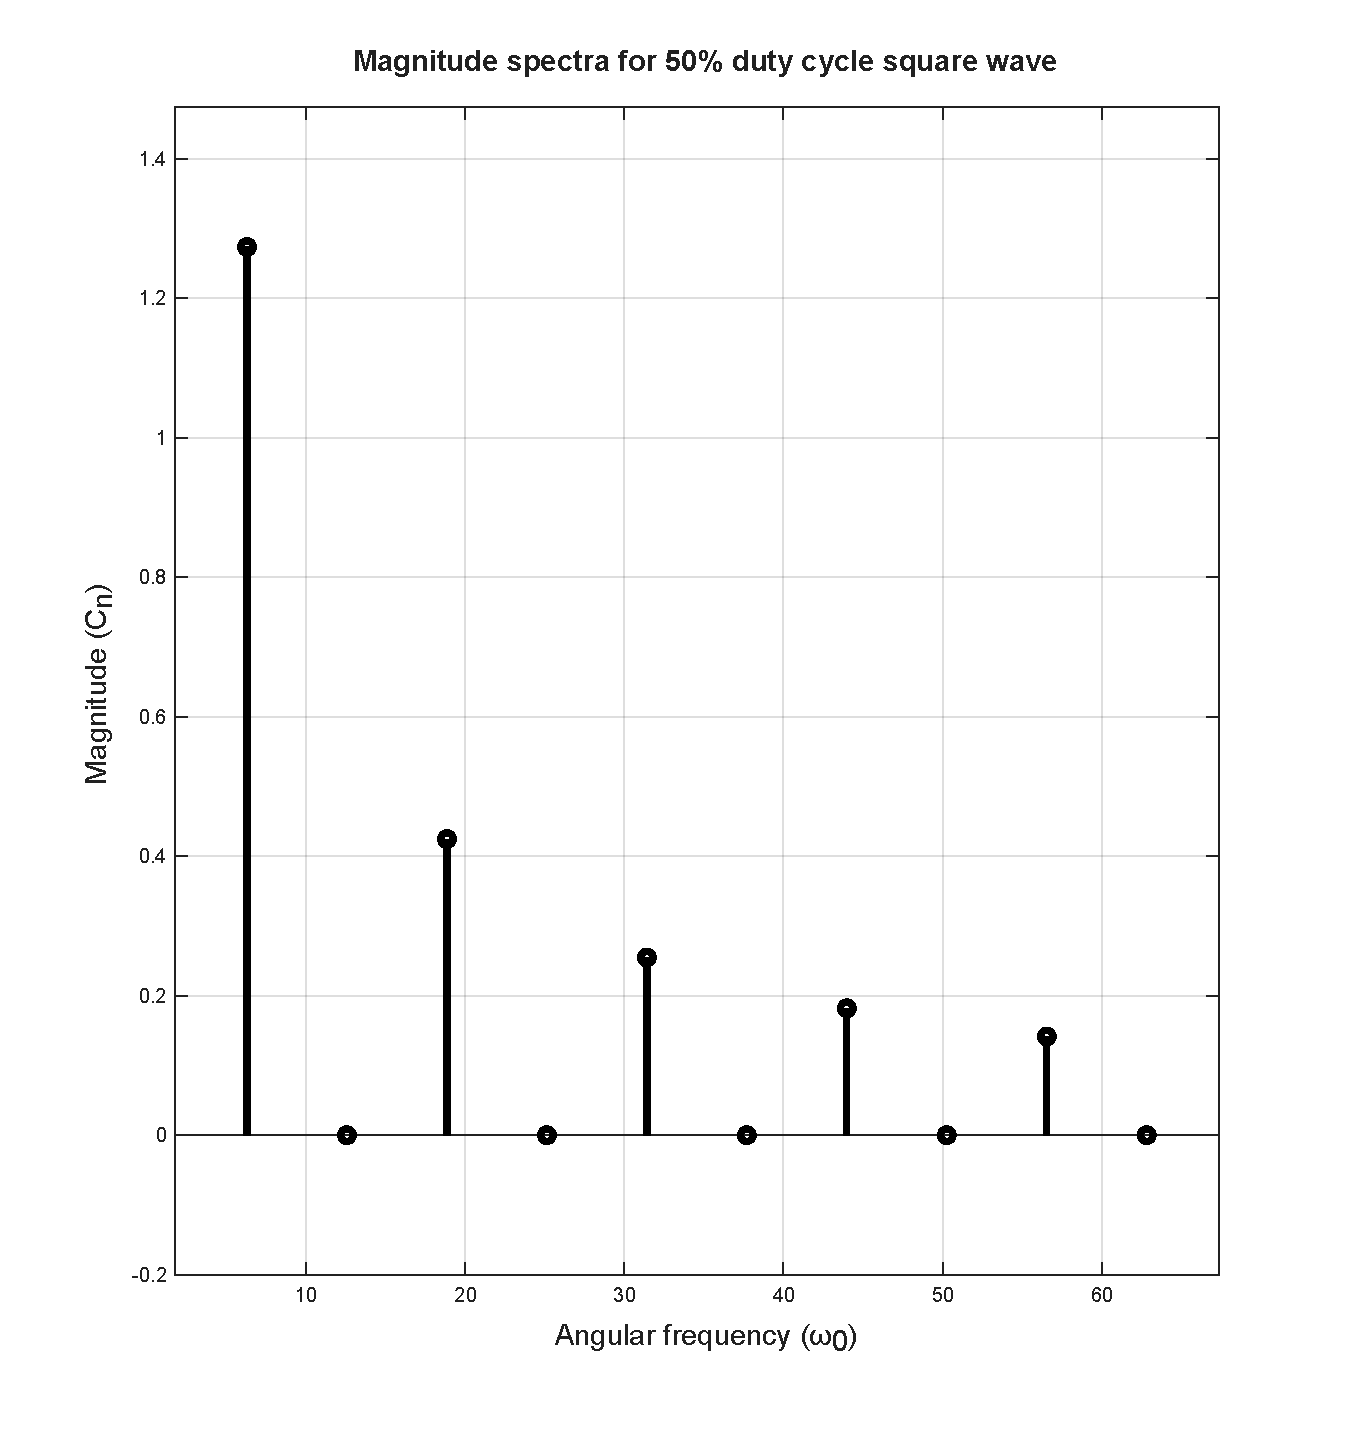
\includegraphics[width=10cm]{figures/SquareWave_50_c10_magnitude_spectra.pdf} %sq50 mag
    \caption{Magnitude spectra of the square wave with 50\% duty cycle and ten components}
\end{figure}

\begin{figure}[H]
    \centering
    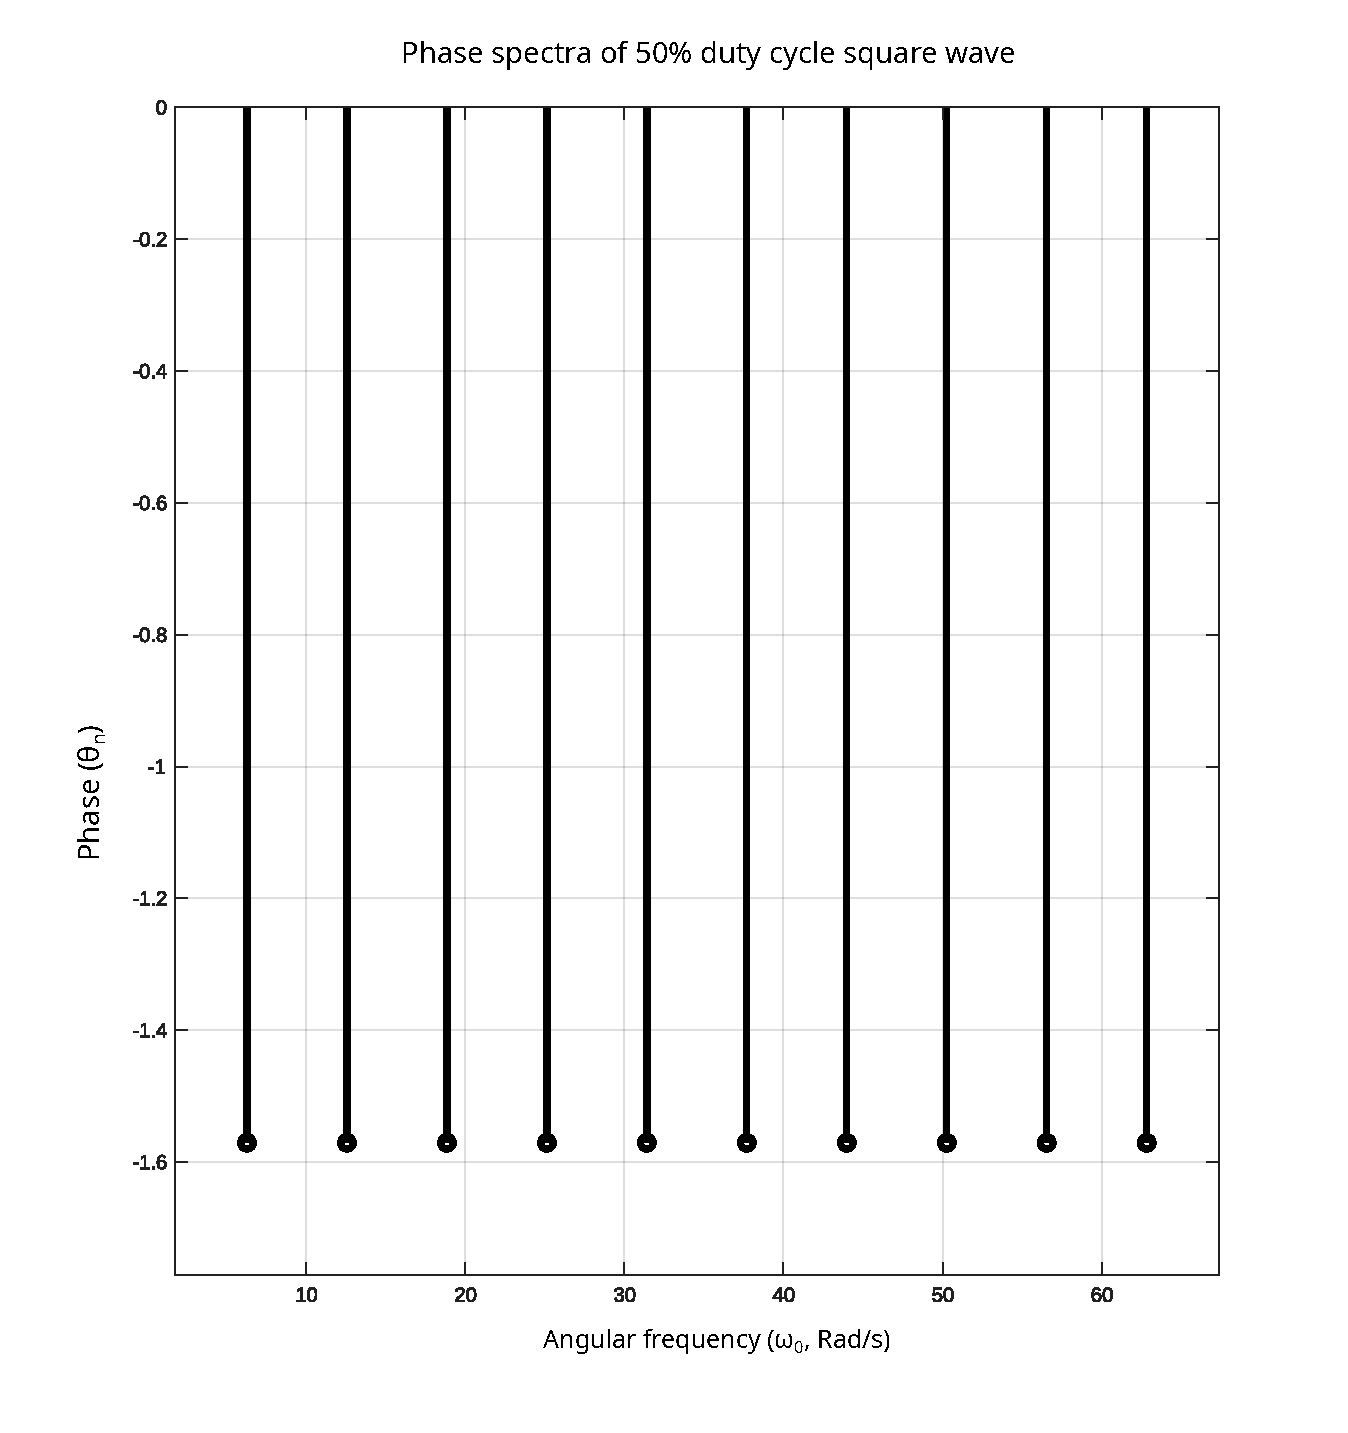
\includegraphics[width=10cm]{figures/SquareWave_50_c10_phase_spectra.pdf} %sq 50 phase
    \caption{Phase spectra for 50\% duty cycle square wave with ten components}
    \label{fig:square50_phase}
\end{figure}


\subsection{Square wave with a 10\% duty cycle}
\label{sec:square10}
Defined similarly to the previous section, this square wave, however, is active for 10\% of the period while the other 90\% is inactive:
\begin{align}
x(t)=\begin{cases}
    1,\quad 0 \leq t < 0.1\\
    0, \quad 0.1 \leq t < 1,
\end{cases}
\end{align}
where $T=1$ and $\omega_0 = 2\pi$.

\begin{figure}[H]
\centering
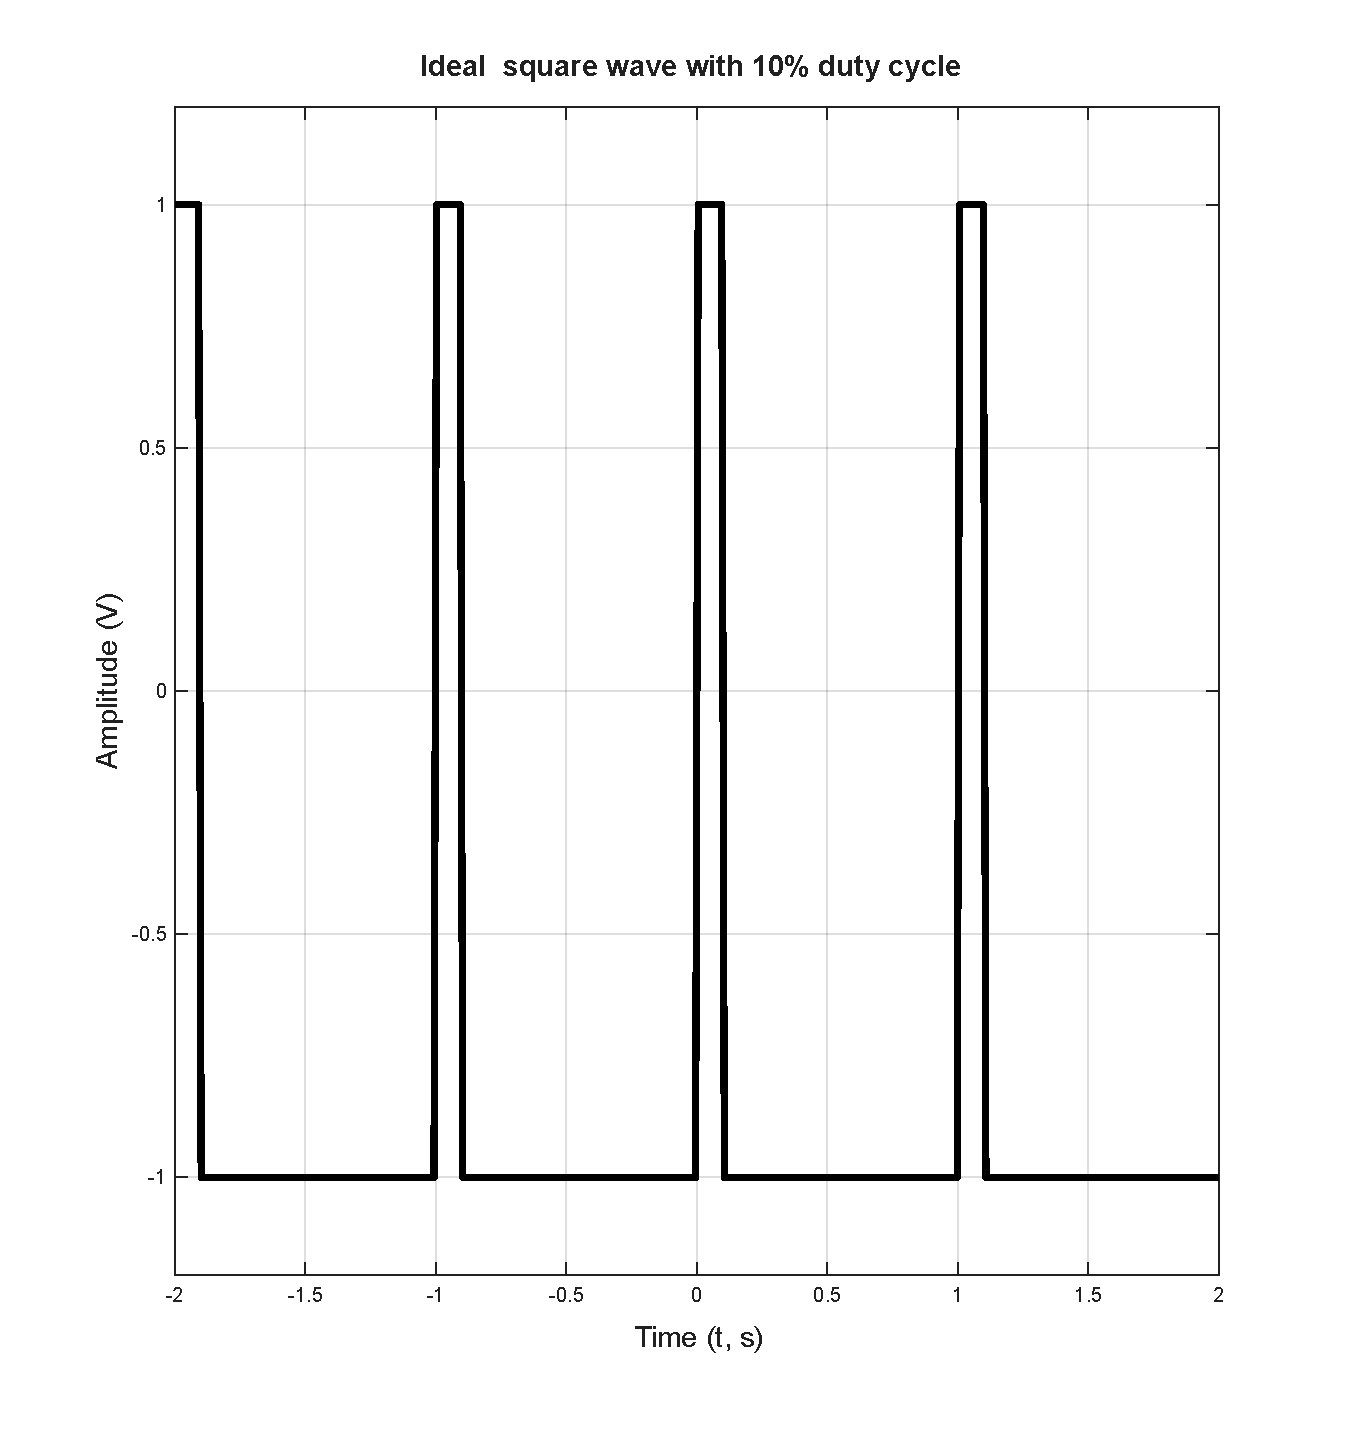
\includegraphics[width=10cm]{figures/SquareWave_10_perfect_series.pdf} %sq10 perf
\caption{Ideal representation of a square wave with a 10\% duty cycle}
\end{figure}

From the \textit{figure} above, it is evident that the function is neither even nor odd. Subsequently, the Fourier expansion will be more complex than the previous sections, and expressions for both $a_n$ and $b_n$ are needed.
\\
Starting with $a_0$, using (\ref{eq:a0def}) yields
\begin{align}
    a_0 &= \frac{2}{T} \int_{0}^{T} F(t) \, dt \nonumber \\
        &= \int_{0}^{0.1} 1 \, dt + \int_{0.1}^{1} (-1) \, dt \nonumber \\
        &= -0.8.
\end{align}

\noindent Then calculating $a_n$ by (\ref{eq:andef}):
\begin{equation} %ADD MORE DEE TAIL dumbass
    a_n = \frac{2}{1} \left[ \int_{0}^{0.1} \cos (n 2 \pi t ) \; dt + \int_{0.1}^{1}- \cos ( n 2 \pi t) \; dt\right]\nonumber
\end{equation}
Evaluating this integral yields:
\begin{align} 
    &= 2 \left[ \frac{1}{2 \pi n} \left(\sin (n 2 \pi t) \bigg|_{0}^{0.1} \right) - \frac{1}{2 \pi n} \left(\sin (n 2 \pi t) \bigg|_{0.1}^{1} \right) \right] \nonumber \\    
    &= \frac{2}{\pi n} \sin (0.2 \pi n).\nonumber \\
\end{align}
Similarly, using (\ref{eq:andef}):
\begin{align}
b_n &= 2 \left[ \int_{0}^{0.1} \sin (n 2 \pi t) \, dt + \int_{0.1}^{1} \sin (n 2 \pi t) \, dt \right] \nonumber \\
 &= 2\left[ \frac{1}{2 \pi n} \left( - \cos (n 2 \pi t)\bigg|_{0}^{0.1} \right) - \frac{1}{2 \pi n} \left( - \cos (n 2 \pi t)\bigg|_{0.1}^{1} \right) \right] \nonumber \\
 &= \frac{1}{\pi n}\left[ -2 \cos (0.2 \pi n) + 1 \right].
\end{align}
The end goal is expressing this expansion in the compact form (\ref{eq:compactfourier}). It is known that $C_0=a_0=-0.8$, and using (\ref{eq:Cn}),
\begin{align}
C_n &= \sqrt{\left( \frac{2}{\pi n} \sin (0.2 \pi n) \right)^2 + \left( \frac{-2}{\pi n} \cos (0.2 \pi n) + \frac{1}{\pi n} \right)} \nonumber \\
\end{align}
Using the trig identity that $\sin^2 x + \cos^2 x = 1$, the expression simplifies to:
\begin{align}
C_n &= \frac{2}{\pi n}\sqrt{ \frac{1}{\pi^2 n^2} - \cos (0.2 \pi n)} \nonumber \\
\end{align}
The final step is finding $\theta_n$:
\begin{align}
    \theta_n &= \arctan \left( \frac{-b_n}{a_n} \right) \nonumber \\
    &= \arctan \left(\frac{2 \cos (0.2 \pi n) -1}{2 \sin (0.2 \pi n)}\right) \\
\end{align}
Filling in all the calculated values of $a_n, b_n, c_n$ and $\theta_n$ into equation  \ref{eq:compactfourier}: %%% ADD REF
\begin{equation}
    x(t) = -0.8 + \sum_{n=1}^{\infty} \frac{2}{\pi n} \sqrt{ \frac{1}{\pi^2 n^2} - \cos (0.2 \pi n)} * \cos \left( 2 n \pi t + \arctan \left( \frac{2 \cos (0.2 \pi n) -1}{2 \sin (0.2 \pi n)} \right) \right)
\end{equation}

\noindent Simulating the above result with only one component has \textit{figure} \ref{fig:square10_c1} as a result. 
\begin{figure}[H]
    \centering
    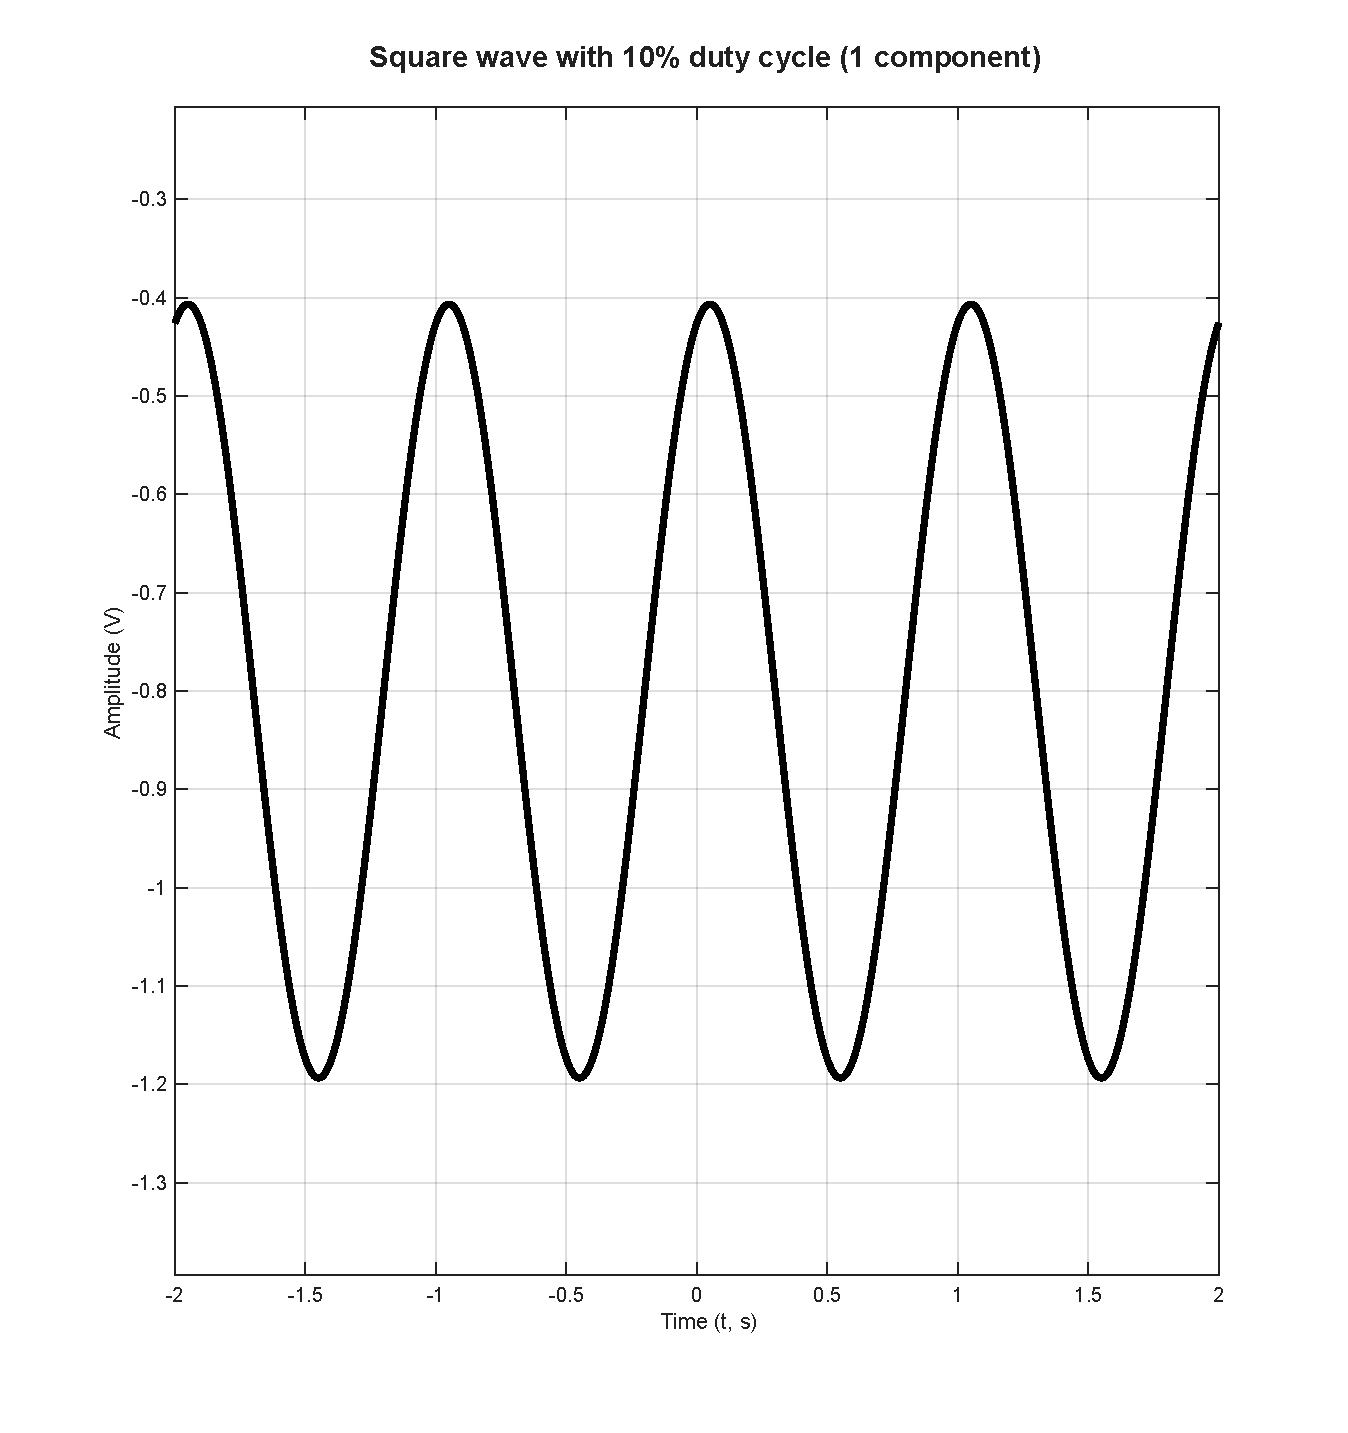
\includegraphics[width=10cm]{figures/SquareWave_10_c1_series.pdf}
    \caption{Plot of the 10\% duty cycle square wave with one component}
    \label{fig:square10_c1}
\end{figure}
The waveform in \textit{figure} \ref{fig:square10_c1} is evidently not an accurate depiction of the 10\% duty cycle square wave. However, with an increasing number of components \textit{figures} \ref{fig:square10_c2} to \ref{fig:square10_c10} are generated.

\begin{figure}[H]
    \centering
    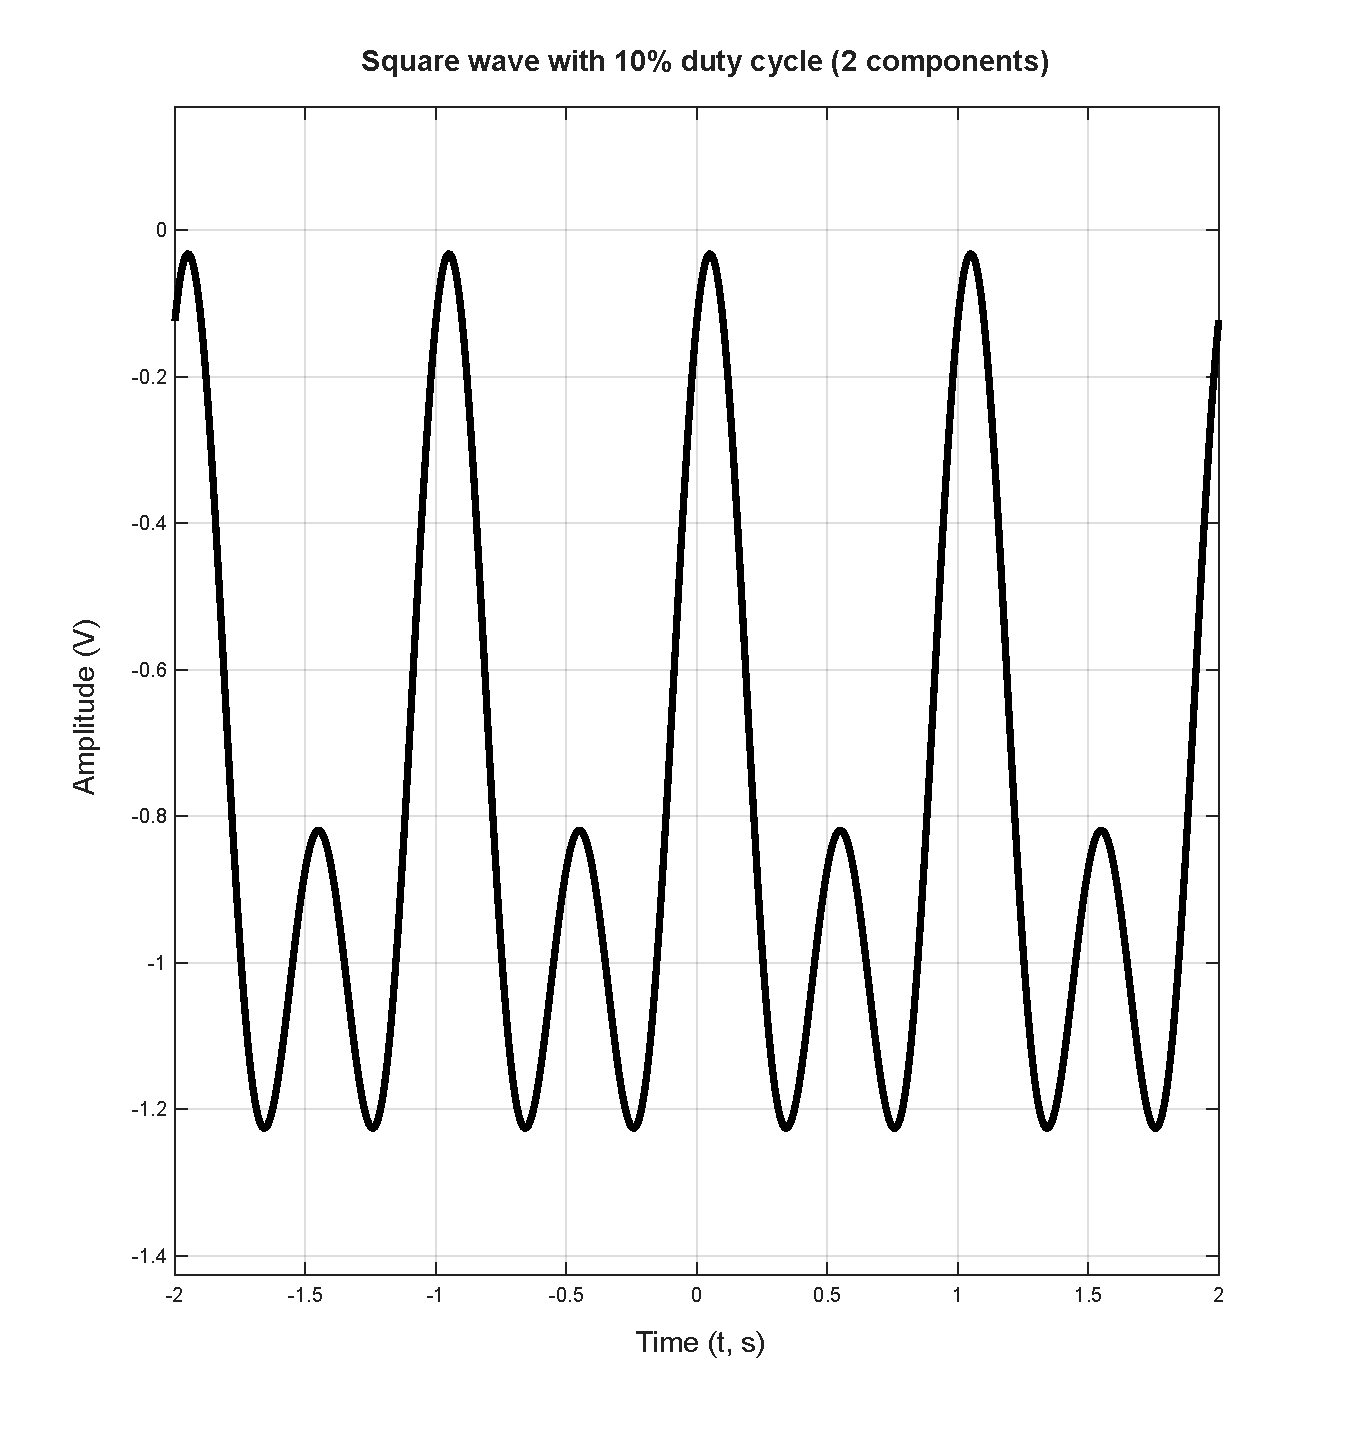
\includegraphics[width=10cm]{figures/SquareWave_10_c2_series.pdf}
    \caption{Plot of the 10\% duty cycle square wave with two components}
    \label{fig:square10_c2}
\end{figure}

\begin{figure}[H]
    \centering
    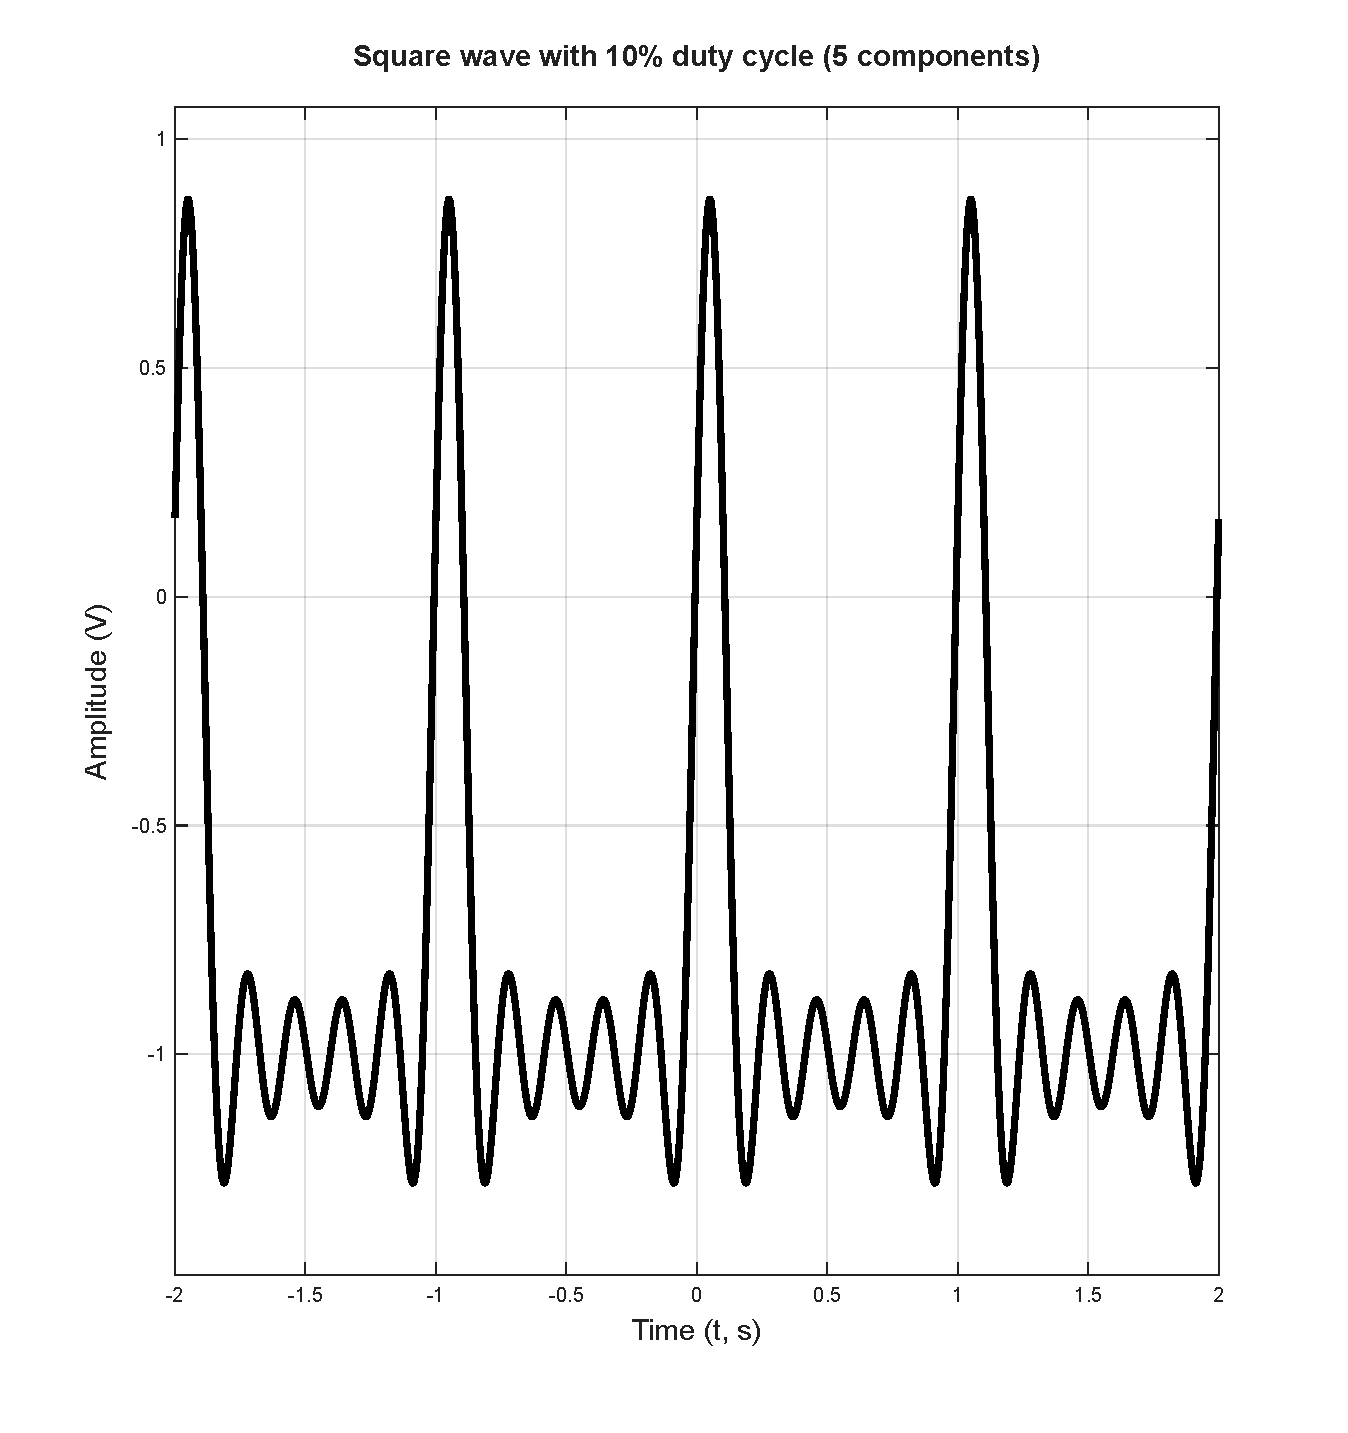
\includegraphics[width=10cm]{figures/SquareWave_10_c5_series.pdf}
    \caption{Plot of the 10\% duty cycle square wave with five components}
    \label{fig:square10_c5}
\end{figure}

\begin{figure}[H]
    \centering
    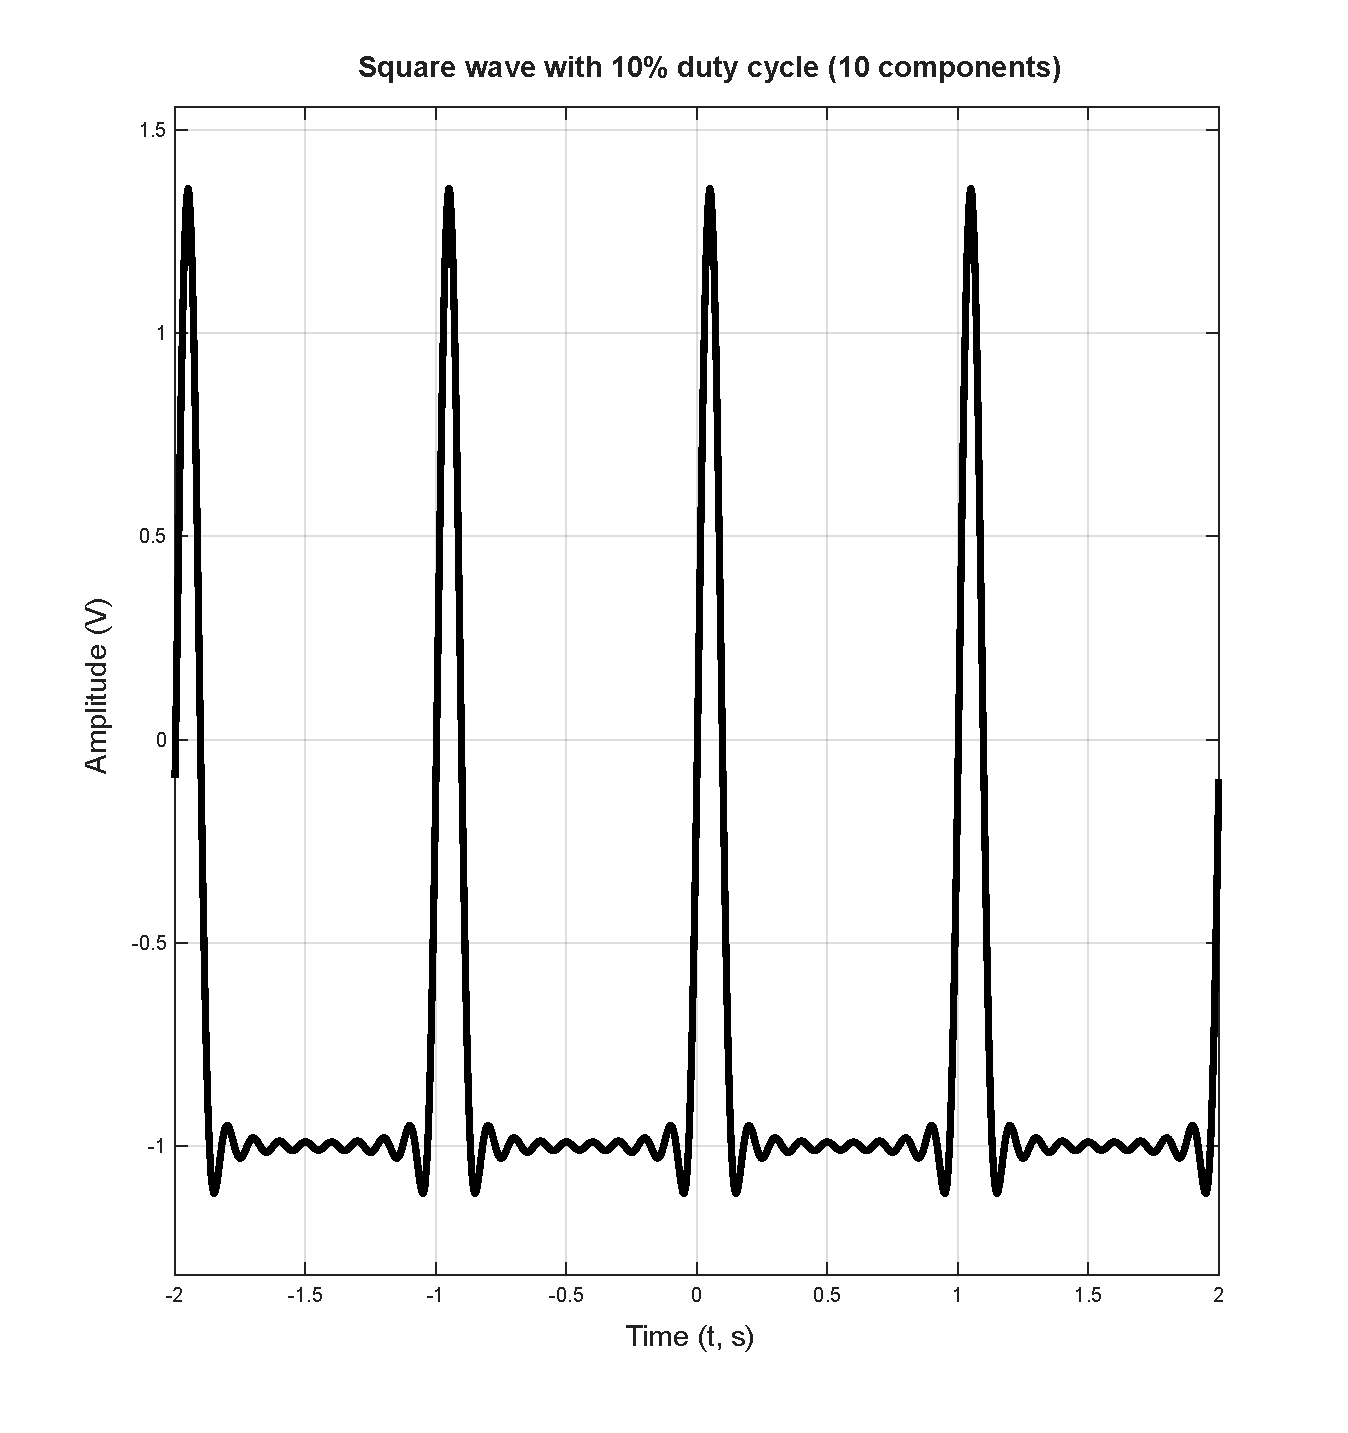
\includegraphics[width=10cm]{figures/SquareWave_10_c10_series.pdf}
    \caption{Plot of the 10\% duty cycle square wave with ten components}
    \label{fig:square10_c10}
\end{figure}

With ten components the waveform looks almost like the ideal, but much more components will be needed to increase the accuracy of the depiction. It seems that the Gibbs phenomenon, as mentioned in the previous section, has a greater effect, which may be due to the shorter time period between discontinuities. However, the phenomenon will always cause only a deviation of 9\% \cite{eli}. Again, it is easy to find necessary information from the FFT, magnitude spectra and phase spectra after applying the Fourier series, as seen in \textit{figures} \ref{fig:square10_mag} to \ref{fig:square10_FFT}.

It should be added that the practical measurements in the lab for this waveform and the sawtooth signal were conducted using an ESP32 (the code is included in Appendix A), so the FFT in \textit{figure} \ref{fig:square10_FFT} may appear more noisy than expected.

\begin{figure}[H]
    \centering
    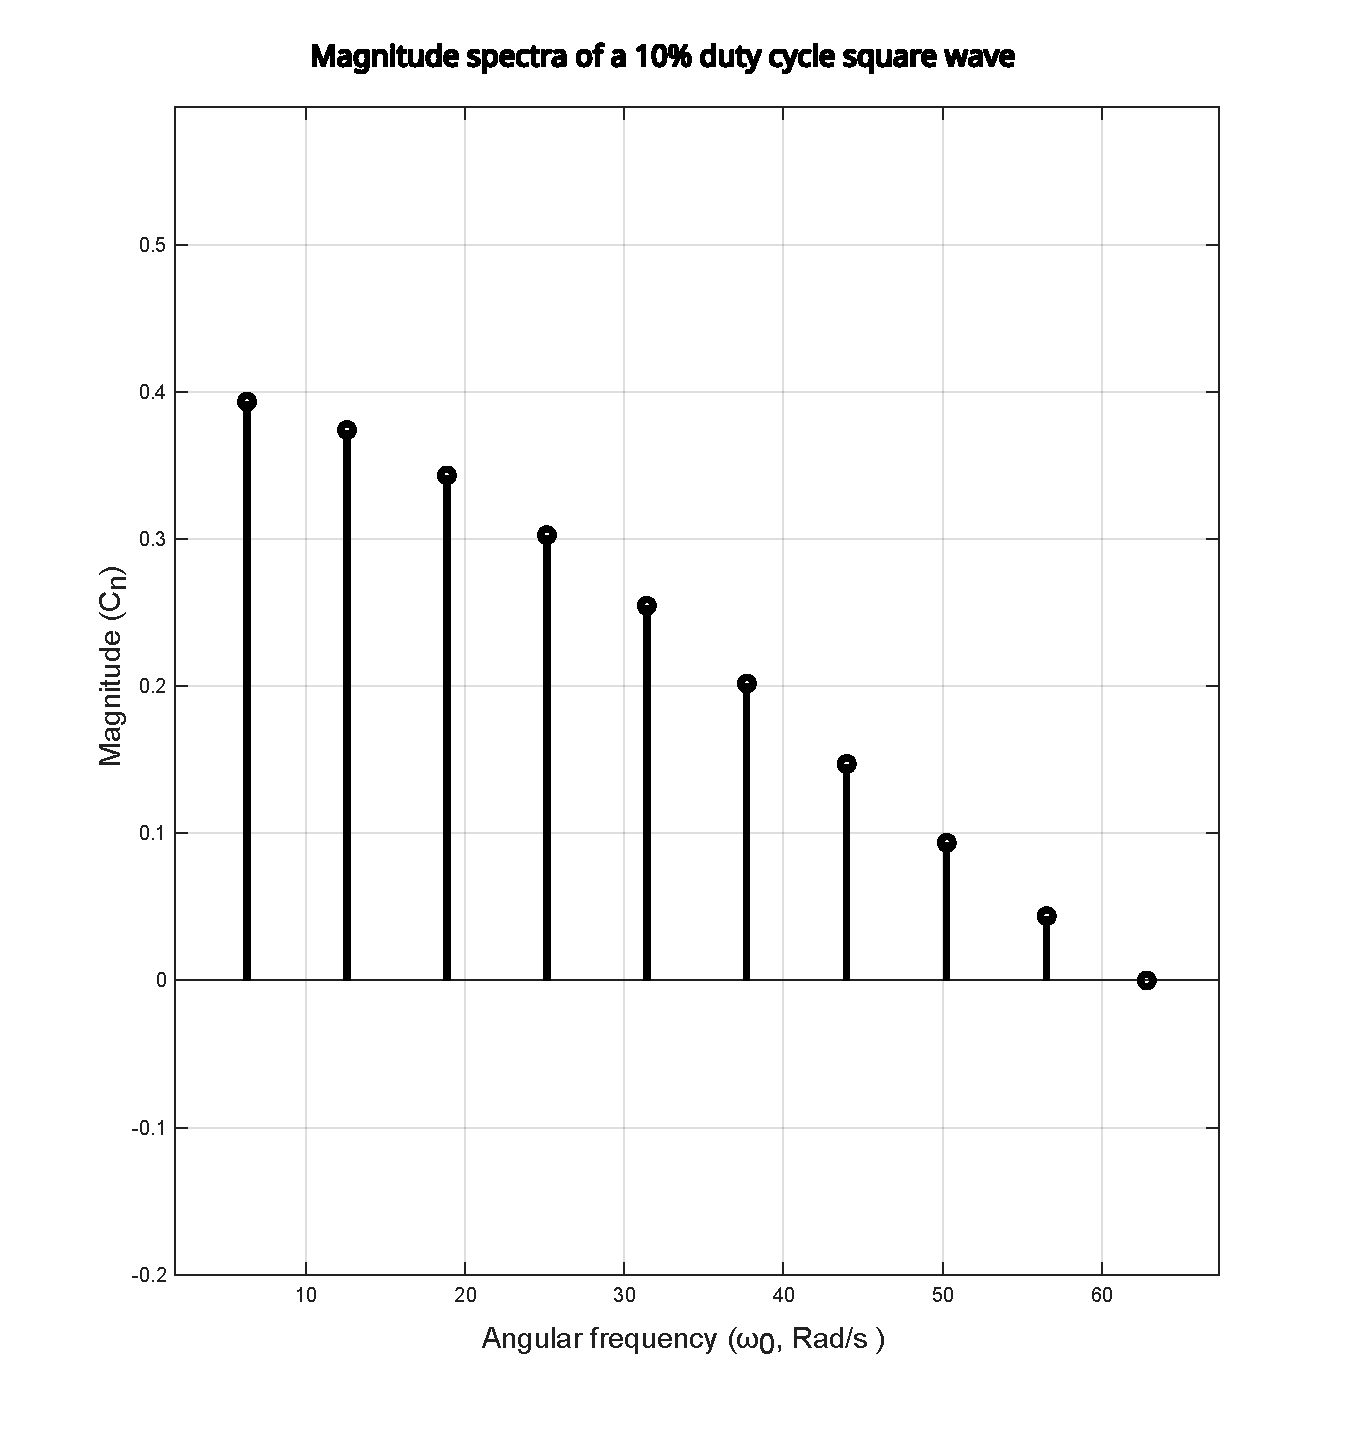
\includegraphics[width=10cm]{figures/SquareWave_10_c10_magnitude_spectra.pdf} %sq50 mag
    \caption{Magnitude spectra of the 10\% duty cycle square wave with ten components}
    \label{fig:square10_mag}
\end{figure}

\begin{figure}[H]
\centering
    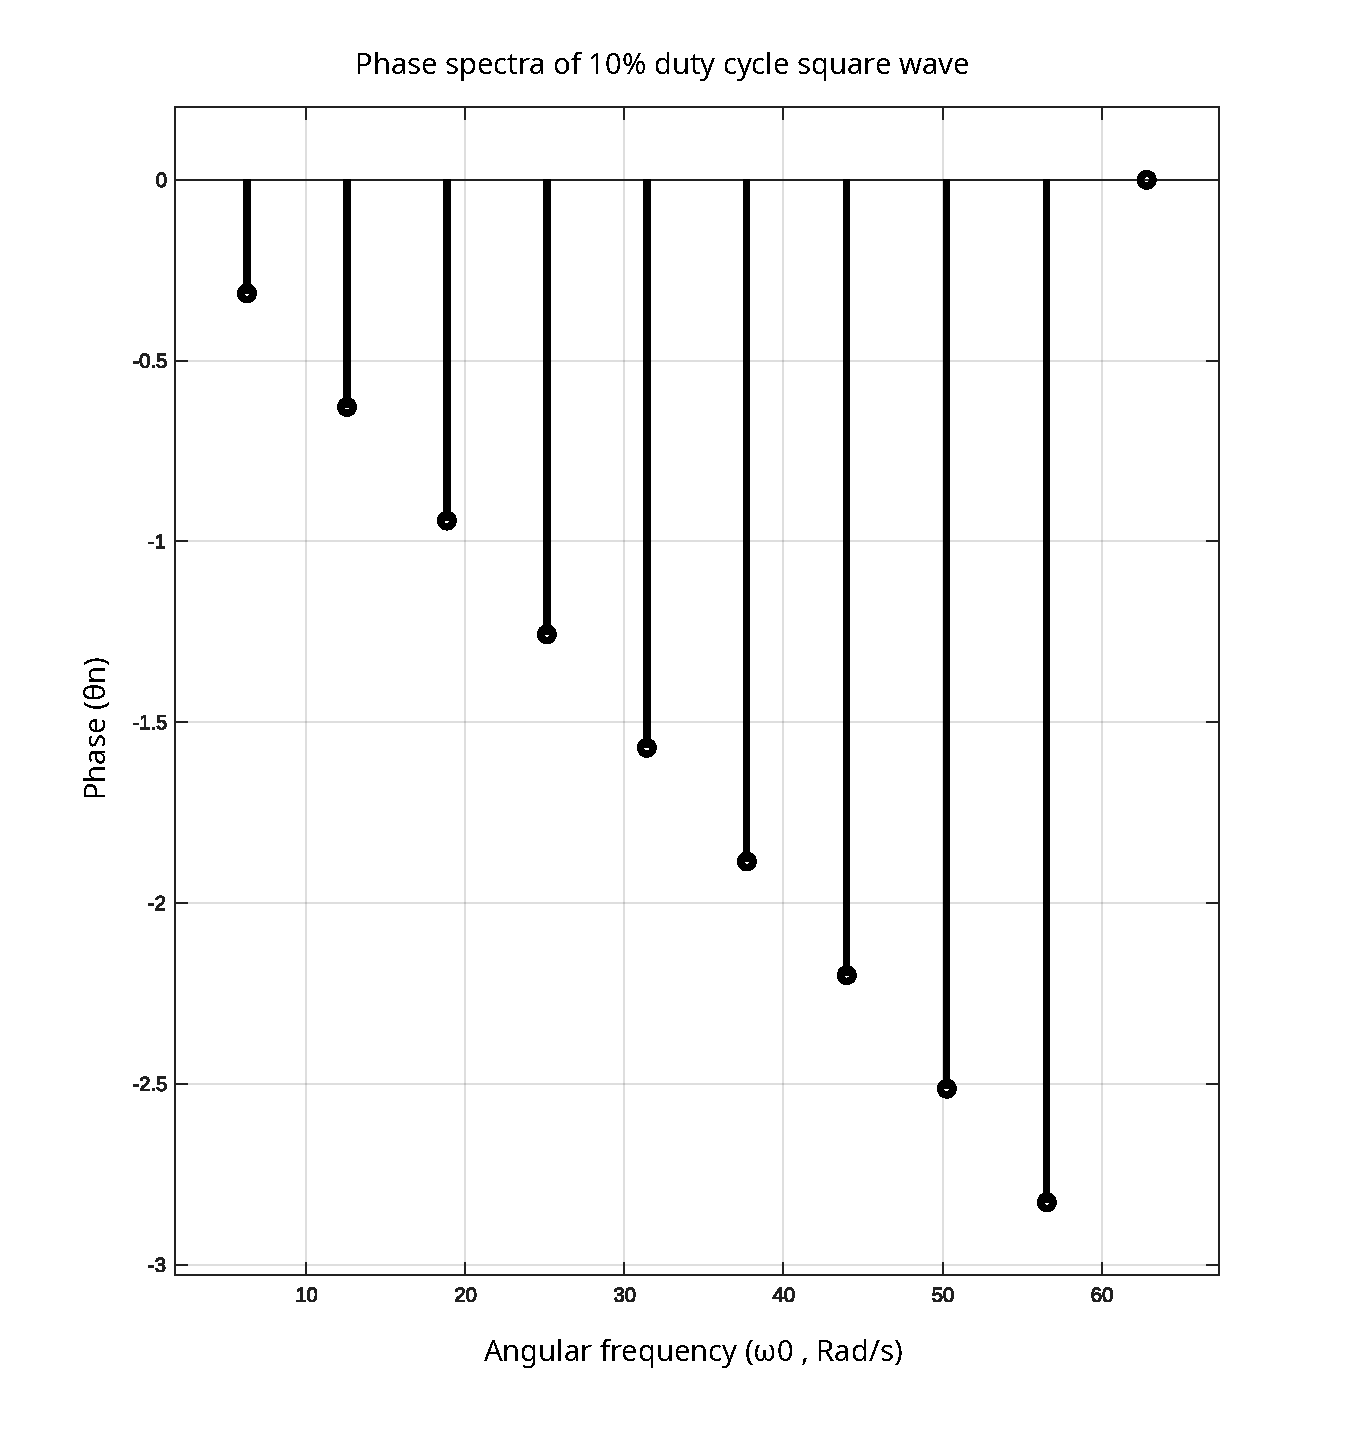
\includegraphics[width=10cm]{figures/SquareWave_10_c10_phase_spectra.pdf} %sq 50 phase
    \caption{Phase spectra for the 10\% duty cycle square wave with ten components}
    \label{fig:square10_phase}
\end{figure}

\begin{figure}[H]
    \centering
    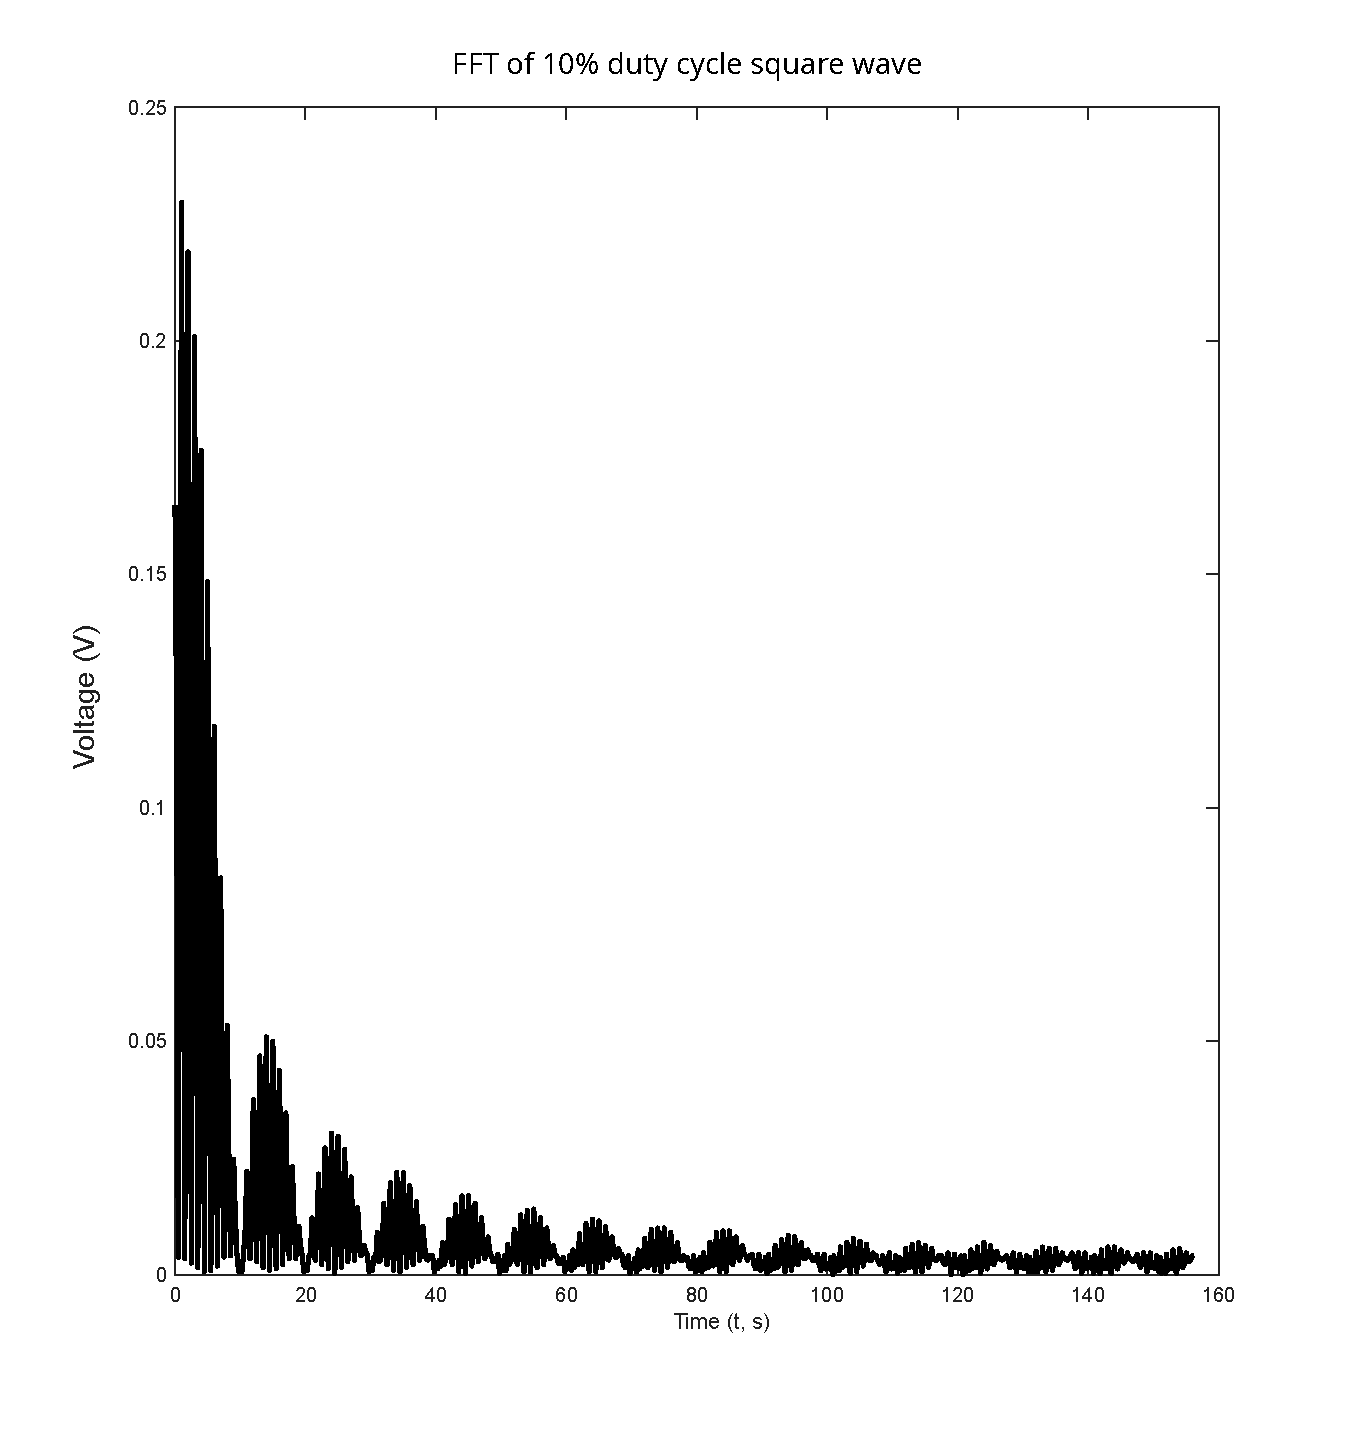
\includegraphics[width=10cm]{figures/Square_10_TEK_plot.pdf}
    \caption{FFT of the 10\% duty cycle square wave}
    \label{fig:square10_FFT}
\end{figure}
\newpage

\subsection{Sawtooth wave}
\label{sec:sawtooth}

A sawtooth waveform consists of a continuous part defined as
\begin{equation}
    x(t)= t, \; 0 \leq t \leq 1,
\end{equation}
after which it immediately drops back to 0, shown in \textit{figure \ref{fig:sawtooth_perf}}. For this analysis, a period of $T=1 s$ and frequency of $\omega_0 = 2\pi$, is considered. This section will also showcase the usage of the exponential form of the Fourier series (\ref{eq:exponentialfourier}).

\begin{figure}[H]
\centering
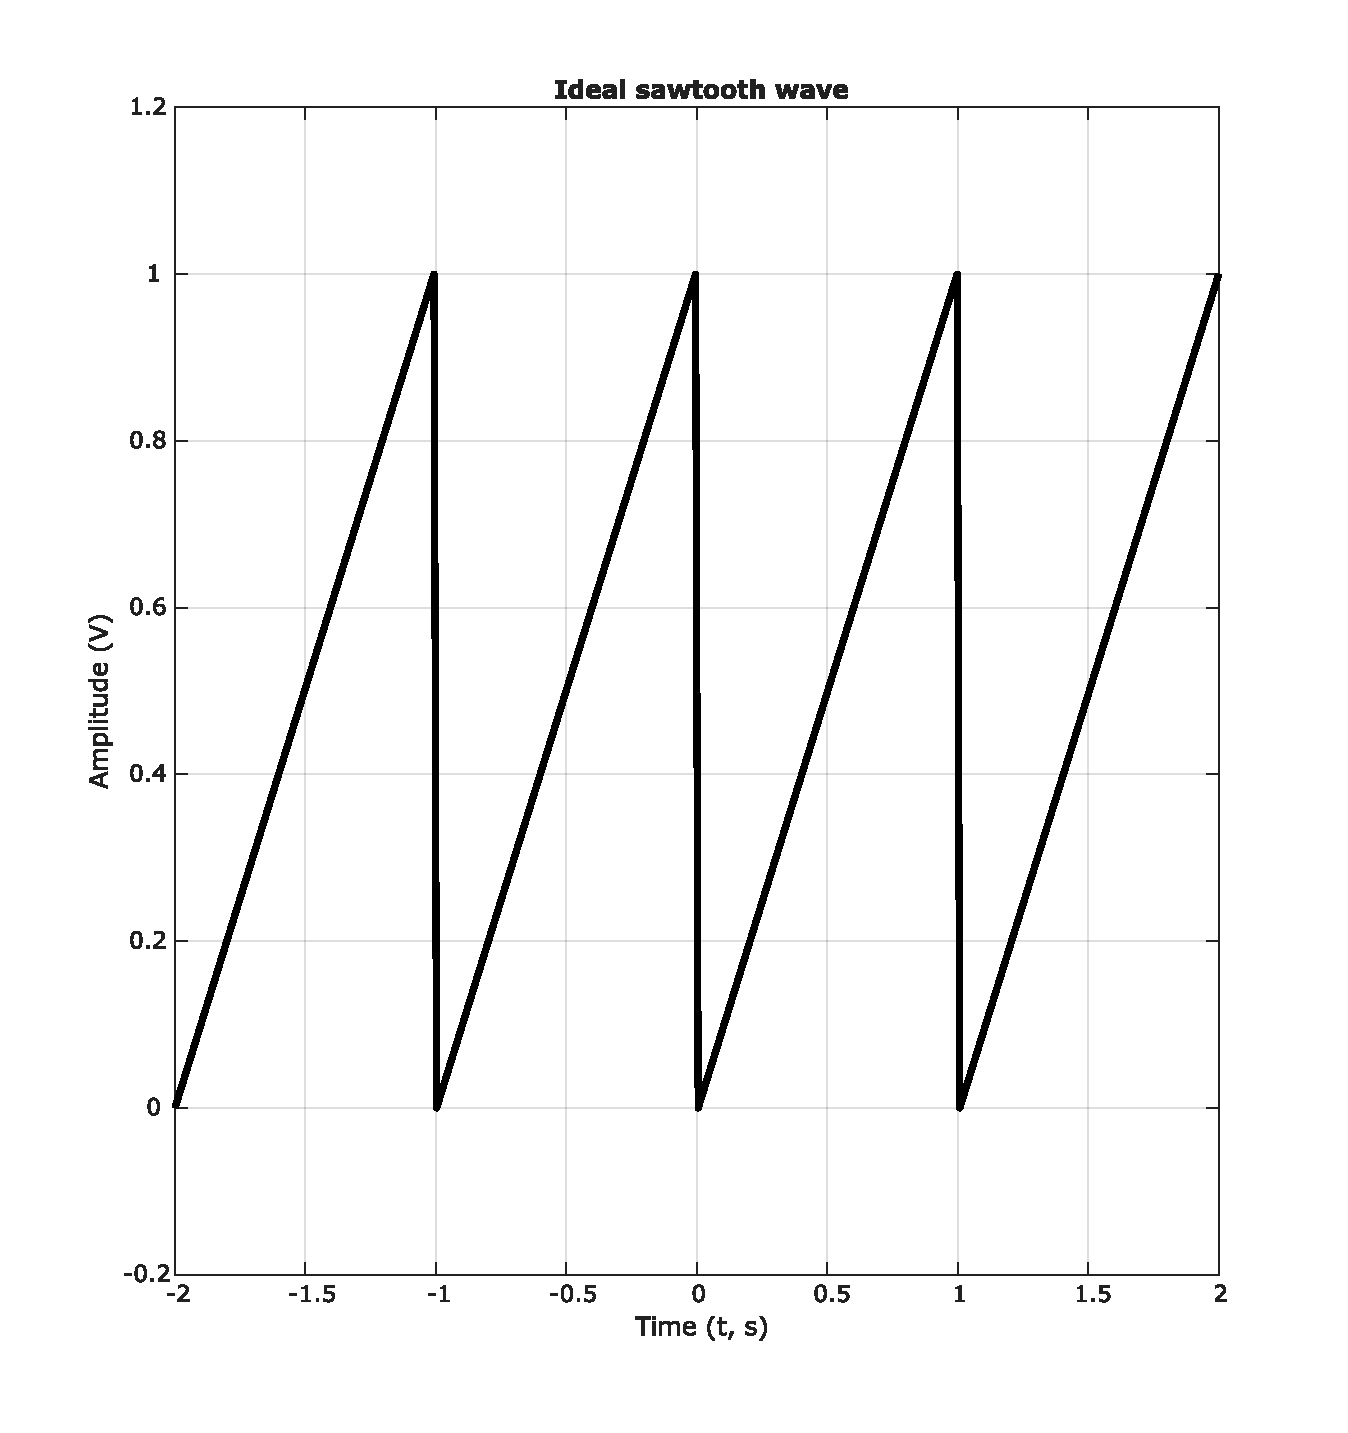
\includegraphics[width=10cm]{figures/SawtoothWave_perfect_series.pdf} %saw t perf
\caption{The ideal representation of a sawtooth waveform}
\label{fig:sawtooth_perf}
\end{figure}

For the exponential method, it is necessary to find an expression for $D_n$, using (\ref{eq:D_n})
\begin{equation}
\label{eq:Dnp1}
    D_n = \int_{0}^{1} t \, e^{-jn 2 \pi t} \, dt,
\end{equation}
and solving with integration by parts (\ref{eq:Dnp1}) becomes
\begin{align}
    D_n &= t * \frac{j}{n 2 \pi} e^{-j n 2 \pi t} \bigg|_{0}^{1} - \int_{0}^{1} \frac{j}{n 2 \pi}e^{-j n 2 \pi t} \, dt \nonumber \\
    &= \frac{j}{n 2 \pi} e^{-j n 2 \pi} + \frac{1}{n^2 4 \pi^2}e^{-j n 2 \pi} \nonumber \\
    &= e^{-j2\pi n}\left( \frac{j}{2 \pi n} + \frac{1}{4 \pi^2 n^2} \right).
\end{align}
By inspection it can be deduced that $D_0=\frac{1}{2}$.
Substituting our $D_n$ value into equation (\ref{eq:exponentialfourier}) and simplifying yields:
\begin{equation}
\label{eq:sawtooth_fourier}
    x(t) = \sum_{n = -\infty}^{\infty} \left( \frac{j}{2 \pi n} + \frac{1}{4 \pi^2 n^2} \right) e^{j2\pi n (t-1)}.
\end{equation}

Plotting (\ref{eq:sawtooth_fourier}) with an increasing amount of components (1, 2, 5 and 10), results in \textit{figures} \ref{fig:sawtooth_c1} to \ref{fig:sawtooth_c10}.

\begin{figure}[H]
    \centering
    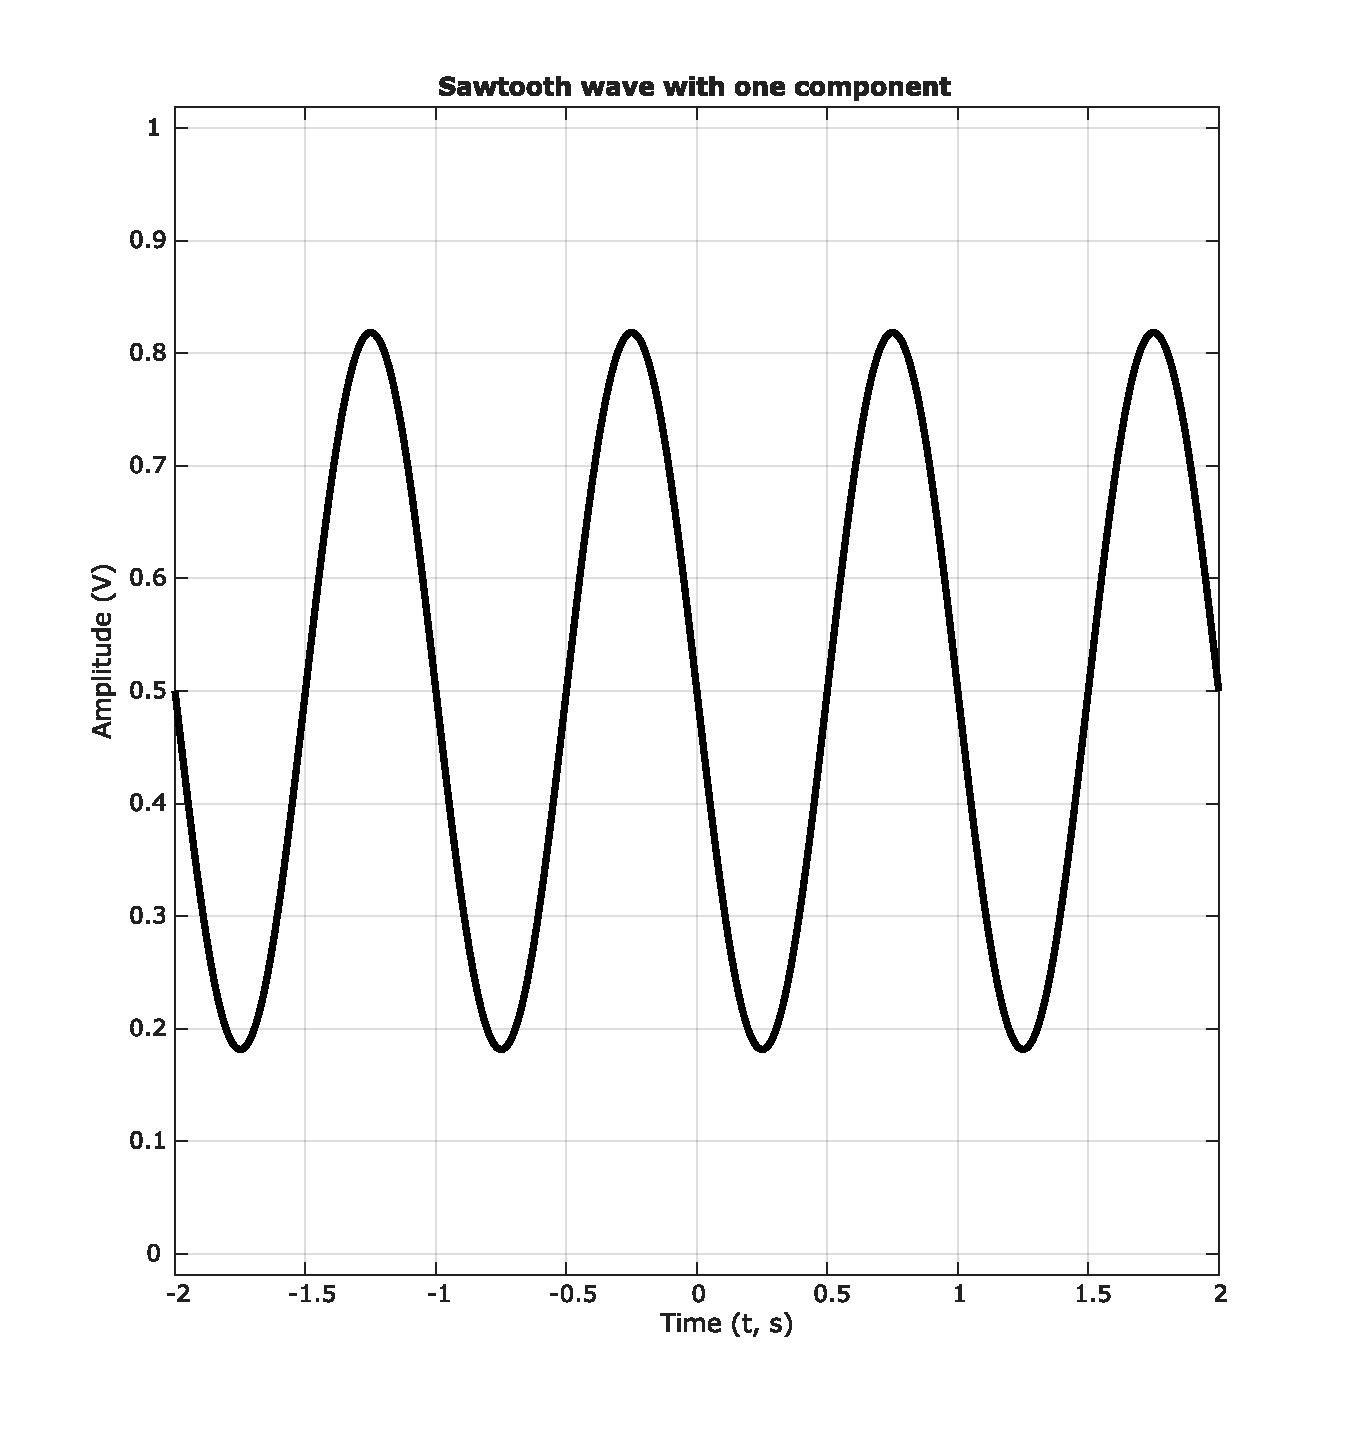
\includegraphics[width=10cm]{figures/SawToothWave_c1_series.pdf}
    \caption{Fourier expansion of the sawtooth wave with one component}
    \label{fig:sawtooth_c1}
\end{figure}

\begin{figure}[H]
    \centering
    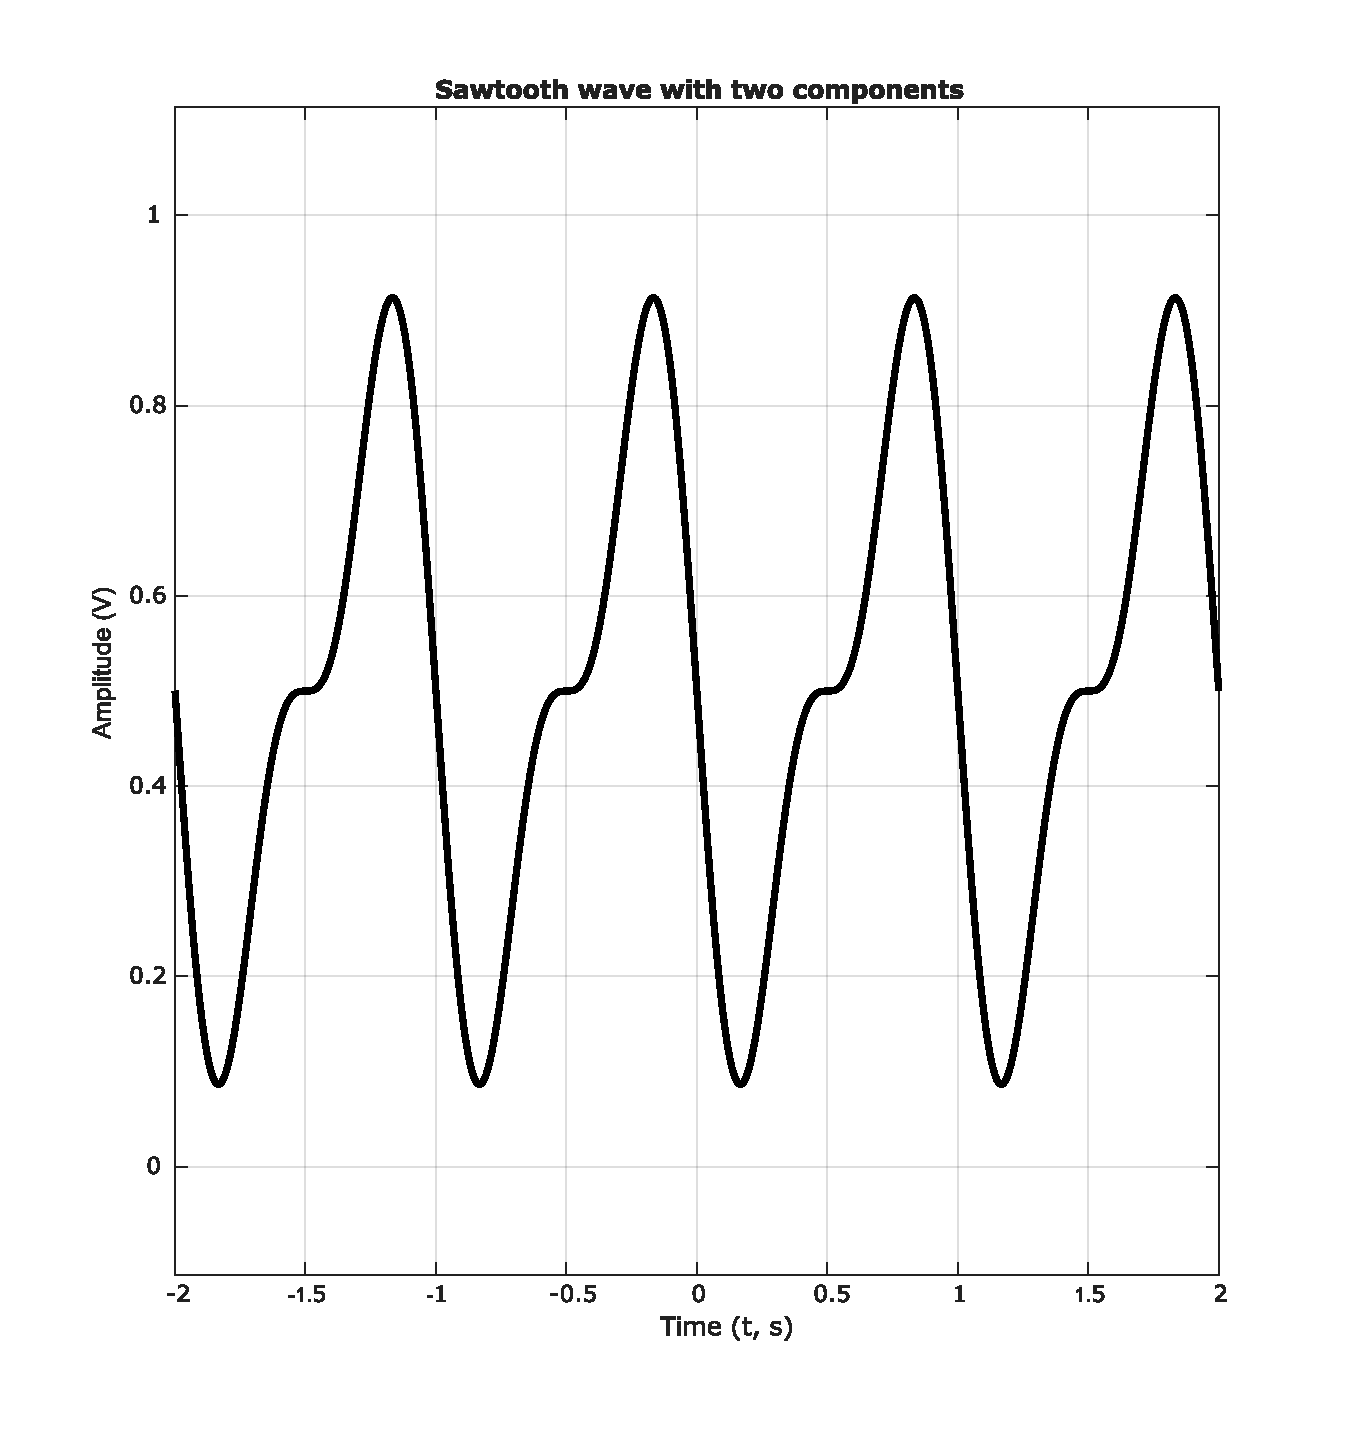
\includegraphics[width=10cm]{figures/SawtoothWave_c2_series.pdf}
    \caption{Fourier series expansion of the sawtooth wave with two components}
    \label{fig:sawtooth_c2}
\end{figure}

\begin{figure}[H]
    \centering
    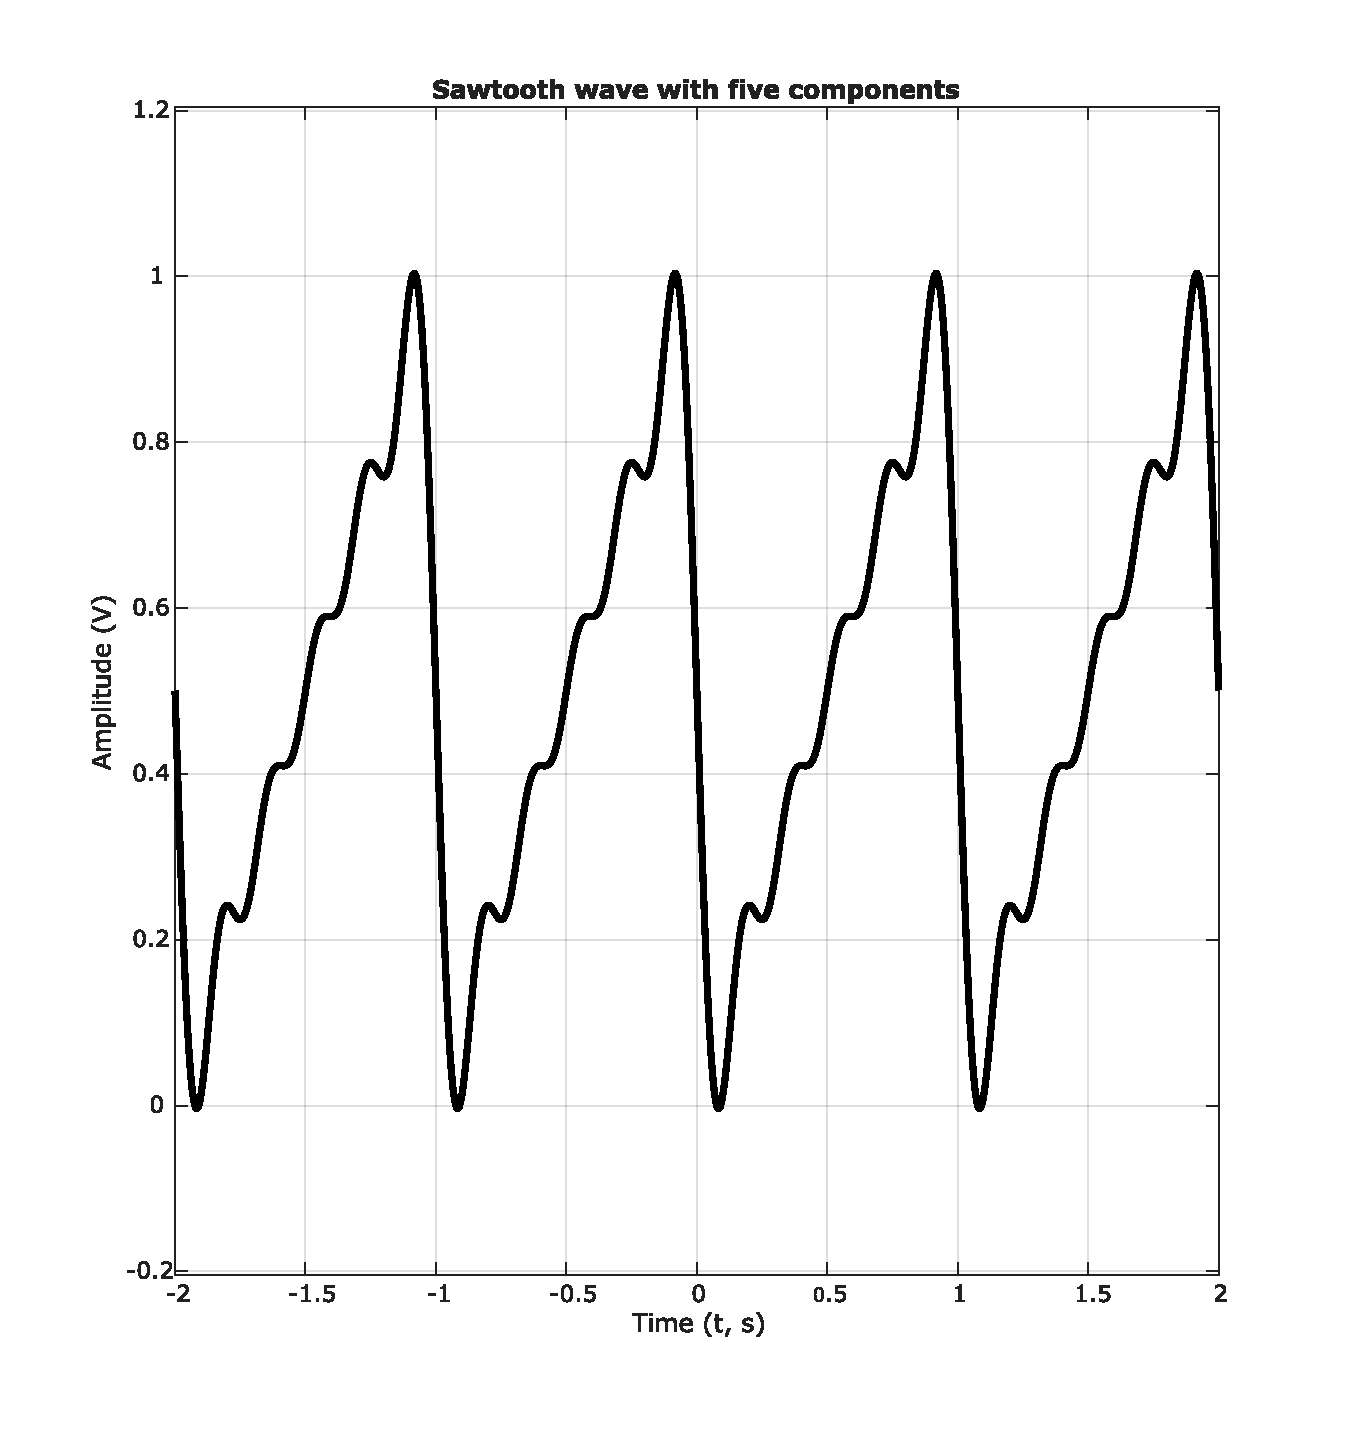
\includegraphics[width=10cm]{figures/SawtoothWave_c5_series.pdf}
    \caption{Plot of the sawtooth waveform with five components}
    \label{fig:sawtooth_c5}
\end{figure}

\begin{figure}[H]
    \centering
    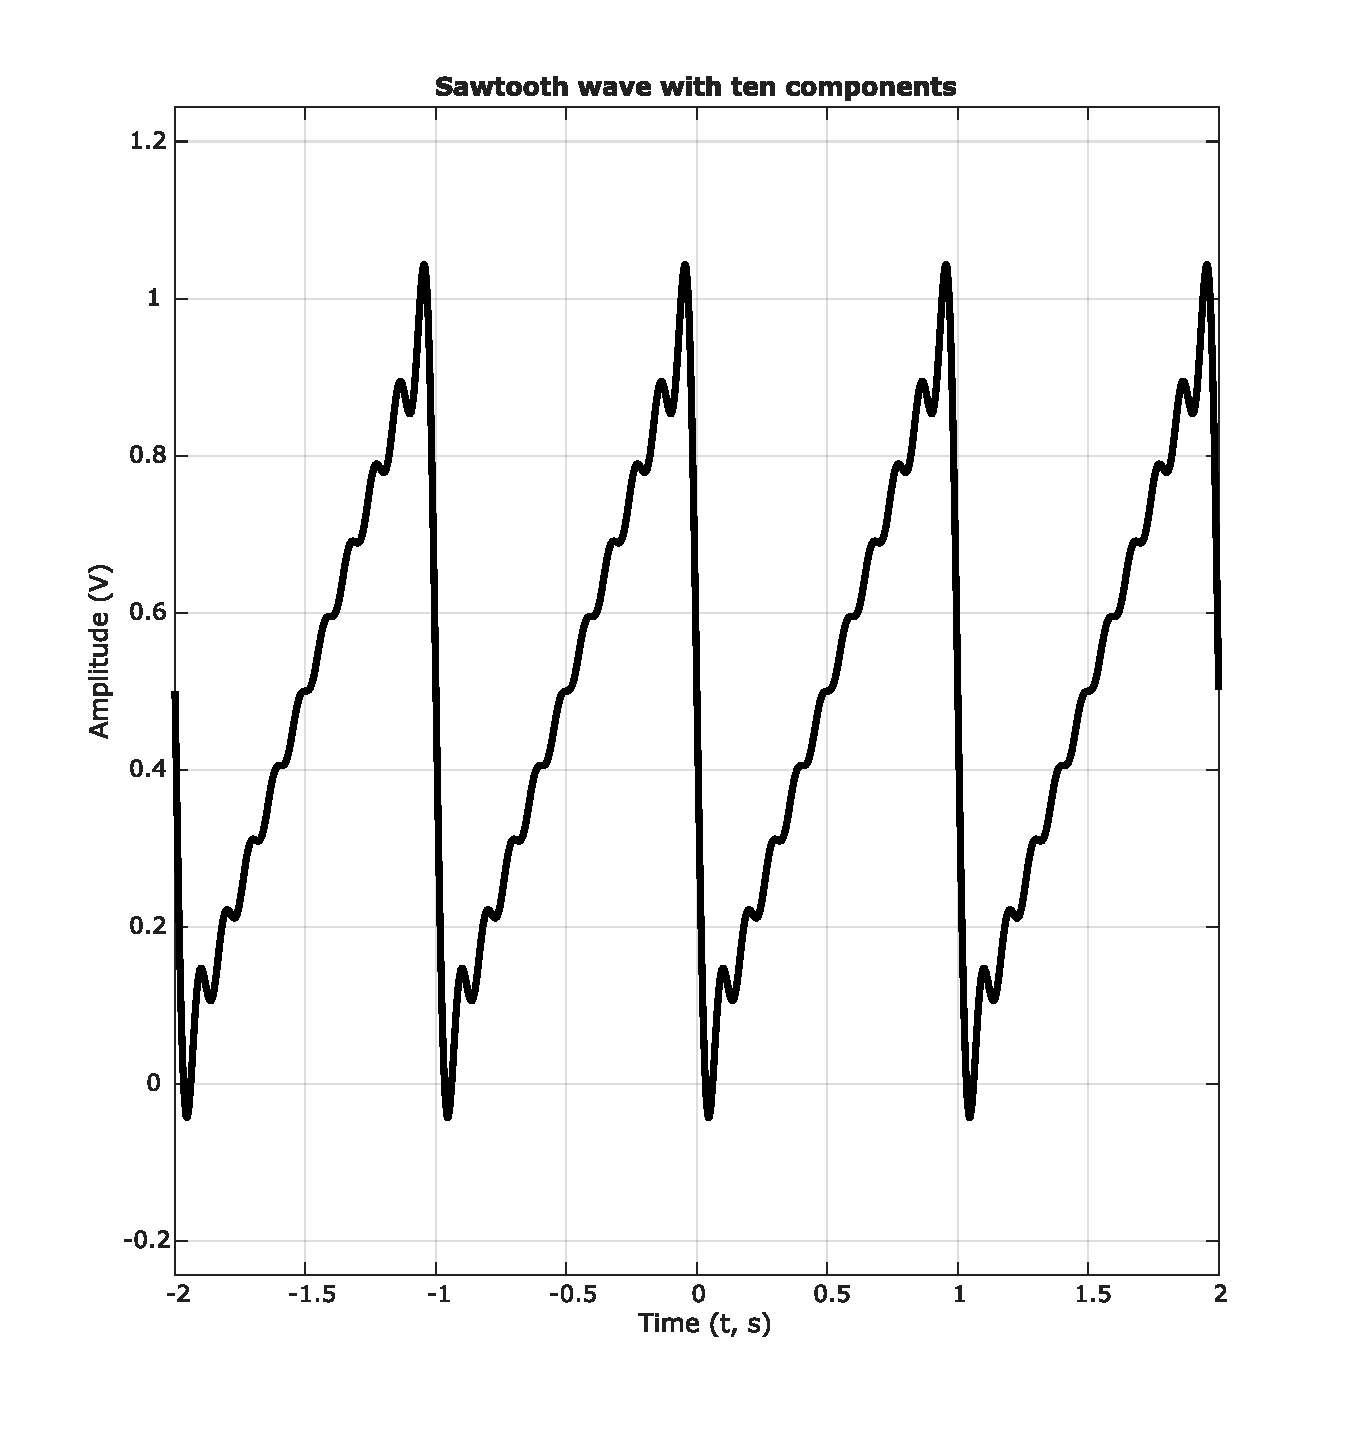
\includegraphics[width=10cm]{figures/SawtoothWave_c10_series.pdf}
    \caption{Plot of the sawtooth waveform with ten components}
    \label{fig:sawtooth_c10}
\end{figure}

Evidently, more components are required to further increase the accuracy, and the aforementioned Gibbs phenomenon occurs. It still does not affect further analysis of the signal using \textit{figures} \ref{fig:sawtooth_mag} to \ref{fig:sawtooth_FFT}. 

\begin{figure}[H]
    \centering
    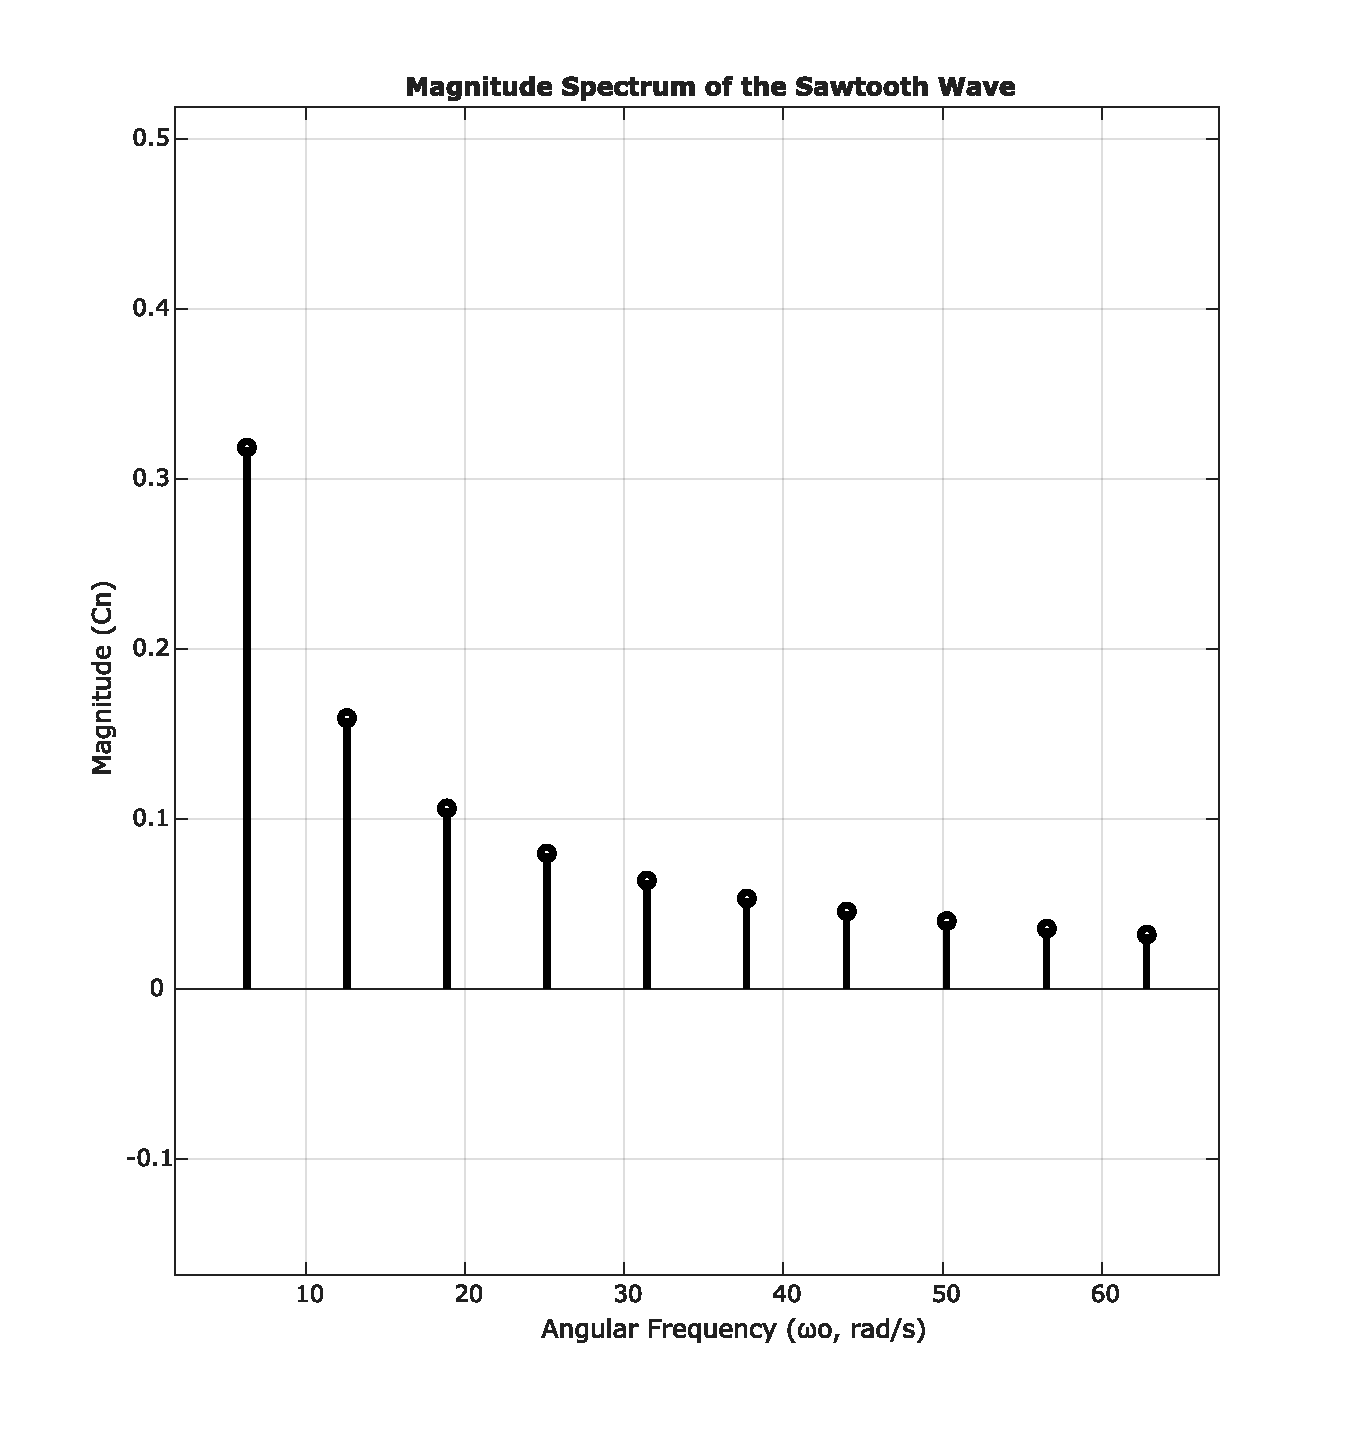
\includegraphics[width=10cm]{figures/SawtoothWave_c10_magnitude_spectra.pdf} %saw t mag
\caption{Magnitude spectra for the sawtooth wave with ten components}
\label{fig:sawtooth_mag}
\end{figure}

\begin{figure}[H]
\centering
    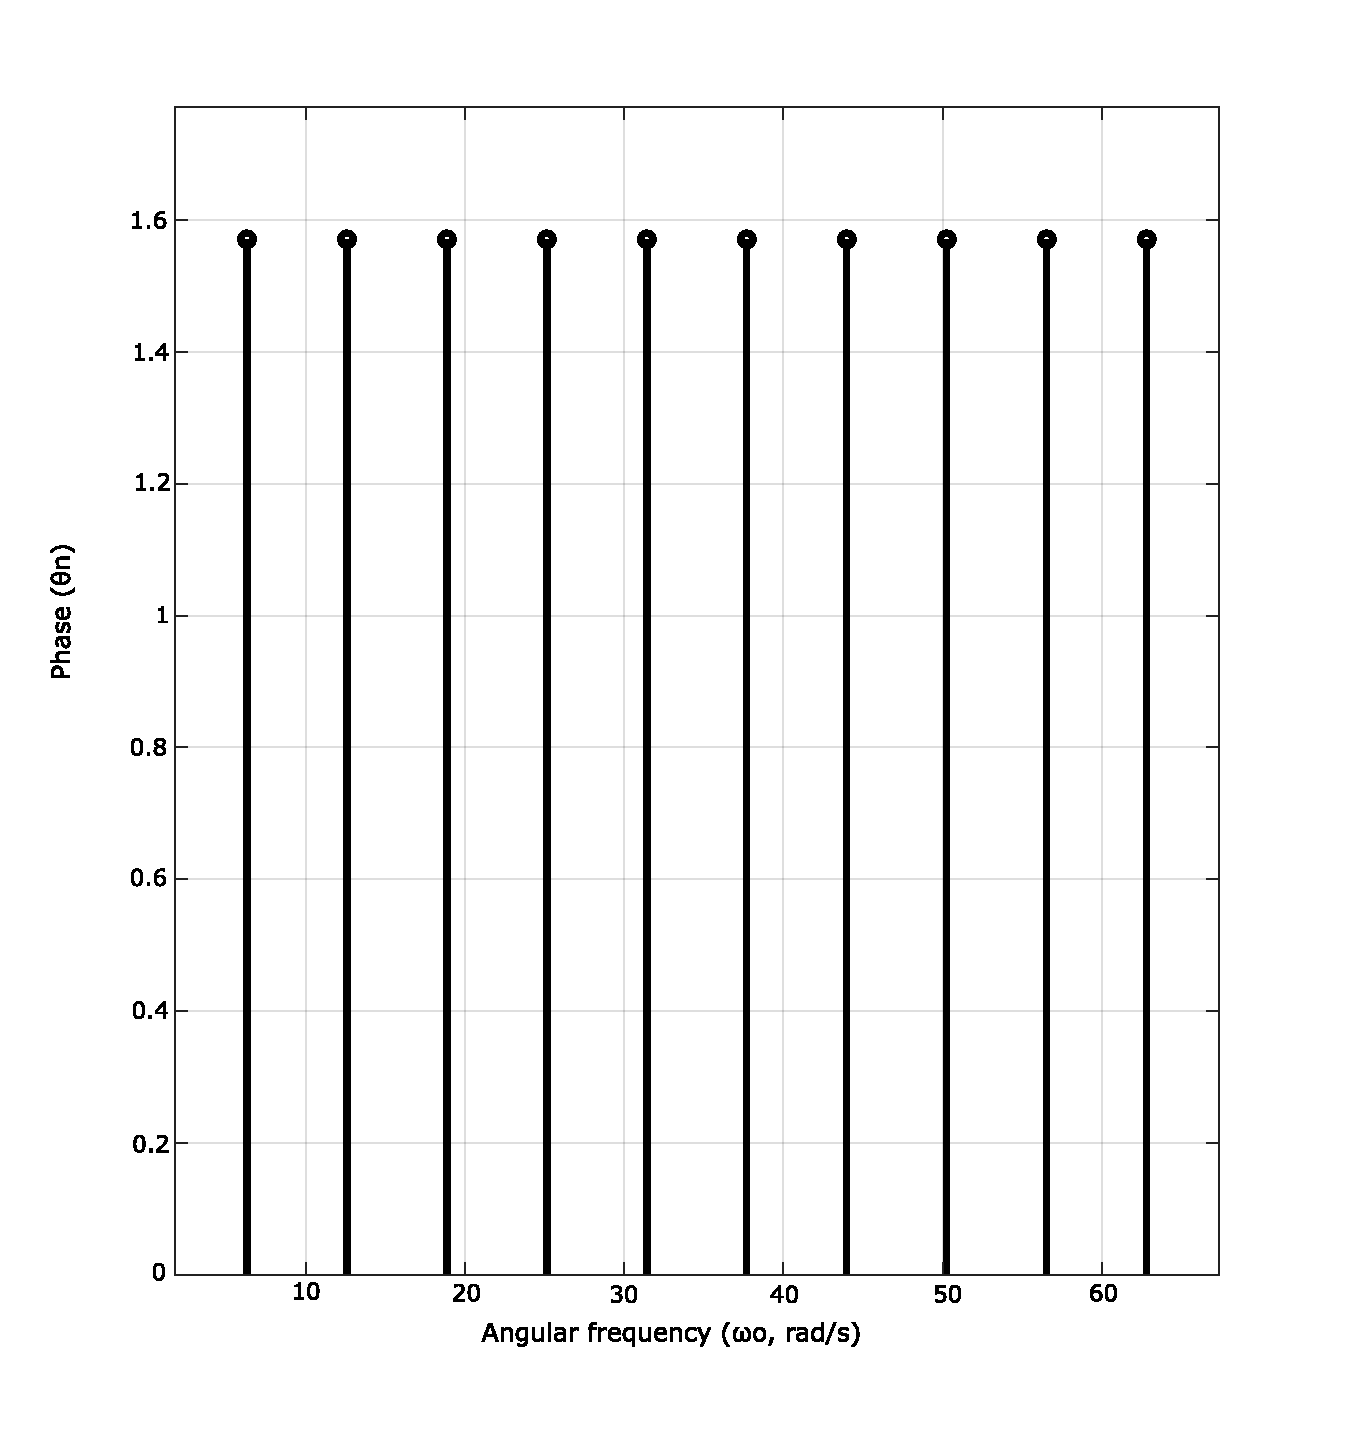
\includegraphics[width=10cm]{figures/SawtoothWave_c10_phase_spectra.pdf} %saw t phase
    \caption{Phase spectra for the sawtooth wave with ten components}
    \label{fig:sawtooth_phase}
\end{figure}

\begin{figure}[H]
    \centering
    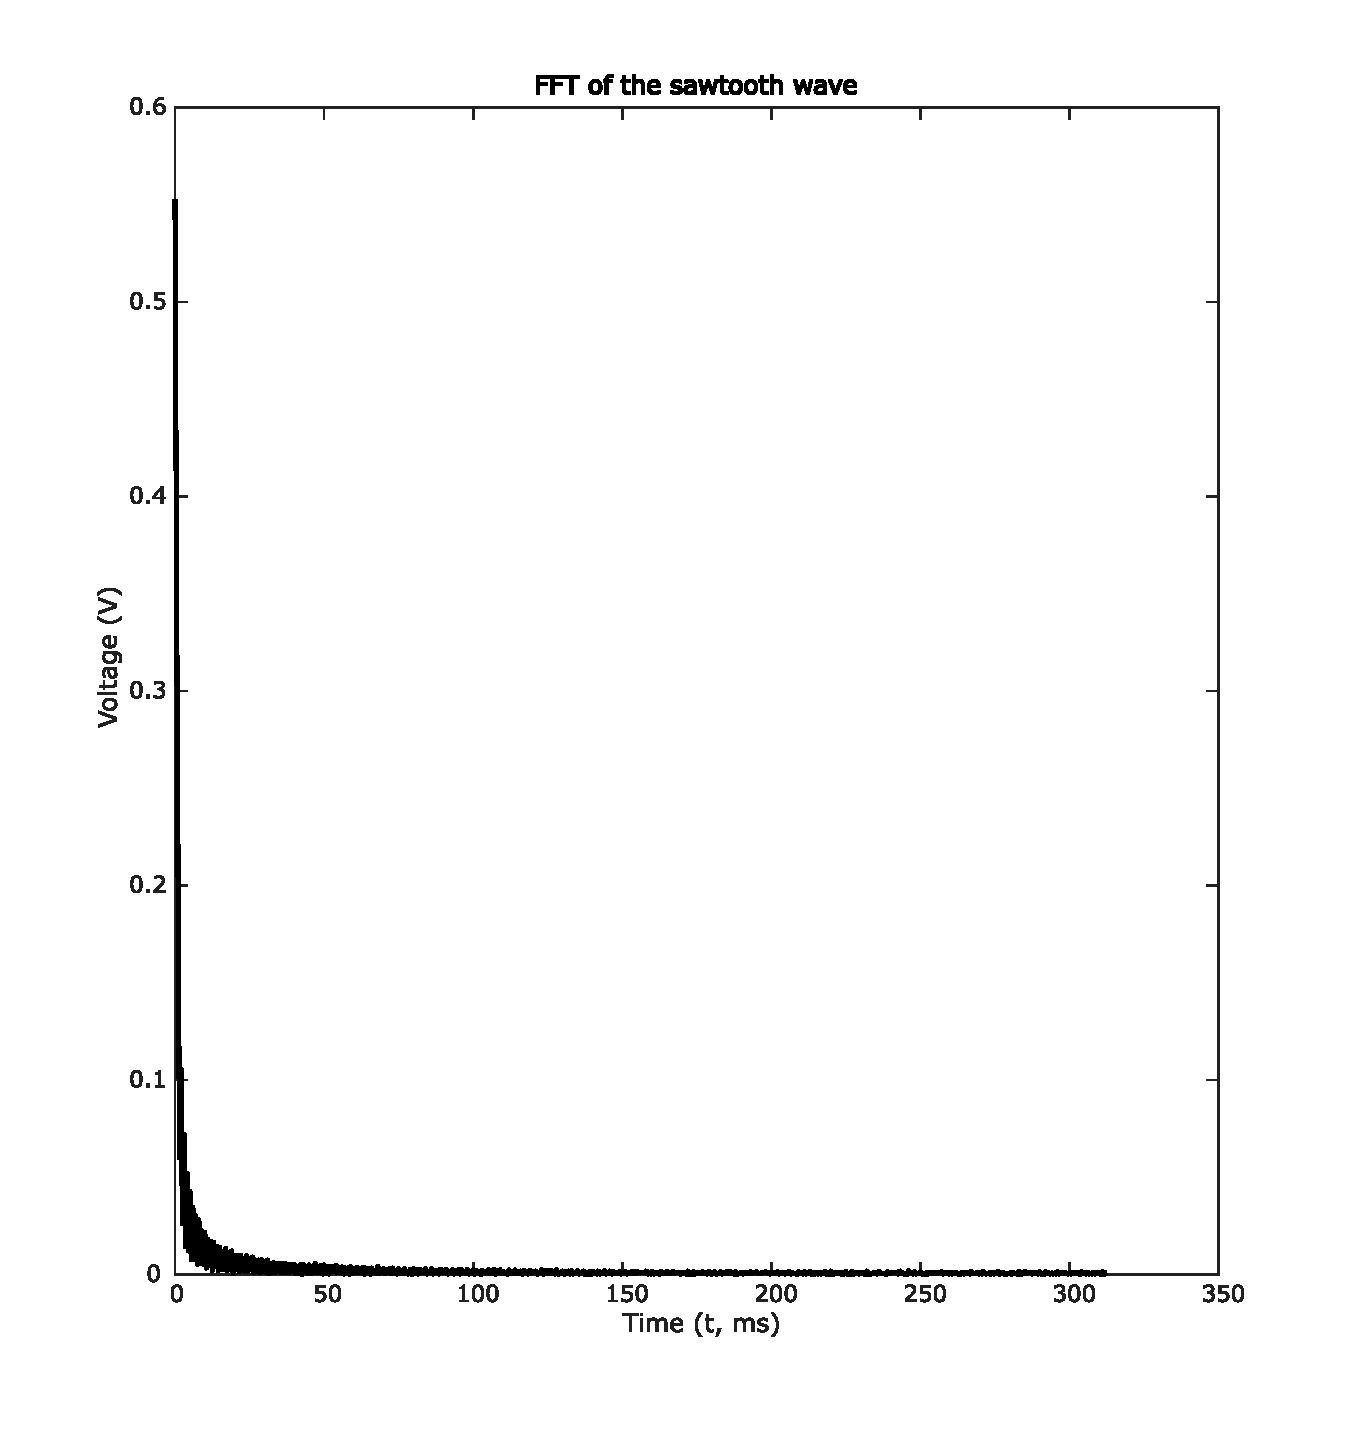
\includegraphics[width=10cm]{figures/SawTooth_ESP_plot.pdf}
    \caption{FFT of the sawtooth waveform}
    \label{fig:sawtooth_FFT}
\end{figure}


\newpage
\section{Conclusion}
\label{sec:conclusion}
By calculating and plotting multiple sinusoidal components with varying amplitudes and periods, it became evident that the Fourier series is an effective method to approximate multiple waveforms. When constructing a discontinuous waveform, the Gibbs phenomenon appears, but after enough components in the Fourier series reconstruction it starts to provide an adequate approximation thereof due to the shrinking nature of the phenomenon, as the amount of components tend to infinity. 

The Fourier series is an important tool in multiple fields, where it can decompose many complicated compound signals into their trigonometric components. It also provides a simple way to simulate any periodic function as long as there are enough components present.
\newpage

% Make the reference font the same size as the rest of the text.
\IEEEtriggercmd{\normalsize}
\IEEEtriggeratref{1}

\bibliographystyle{IEEEtran}%
\bibliography{references}%

%\clearpage
\FloatBarrier

% Use for only one appendix (no titles necessary and no appendix numbers).
% \appendix
% Use for multiple appendices (with appendix numbers).
\appendices
% \section{Abbreviations}
% \label{sec:abbreviations}

\printglossary[type=\acronymtype]

\section{Code}
\label{app:code}

\subsection{MATLAB script for calculating and plotting the Fourier Series}
\label{sec:MATLAB}
  \begin{mdframed}
        \inputminted{Matlab}{./code/prac_1_sim.m}
  \end{mdframed}

\subsection{ESP32 program to simulate a square wave with 10\% duty cycle}
\label{sec:esp_square50}
    \begin{mdframed}
        \inputminted{Arduino}{./code/PWM2.ino}
    \end{mdframed}
    
The Arduino code was uploaded to an ESP32. The square wave code simply multiplies the duty cycle percentage with the period to get an amount of time for which it should hold the digital high state. It subtracts the on-time from the total period to find the off-time. 

Finally, it constantly loops where it switches pin 2 to digital high and then delays by the on-time. After which it switches pin 2 to digital low and delays by the off-time and repeats the loop.

\subsection{ESP32 program to simulate a sawtooth wave}
\label{sec:esp_square10}
    \begin{mdframed}
        \inputminted{Arduino}{./code/SawTooth_Sketch.ino}
    \end{mdframed}
    
The Arduino code above is used to simulate a sawtooth signal. This program is a bit more complex than the previous as it is required to on or off, and to cycle through a range of analogue values.

It uses the the current time and elapsed time to calculate a percentage which is multiplied with the maximum voltage to get the voltage at that particular instant in time. This voltage starts at $0\,$V and linearly rises to about $1\,$V. After one period elapsed it resets the voltage to $0\,$V and restarts the cycle.

\end{document}
